\chapter{Diseño del asistente}
\ihead[]{Capítulo 4: Diseño del asistente}
\label{ch:CH04-Diseno-Asistente}

\section{Ubicación del dispositivo}
En la sección anterior se determinó que el concepto de solución óptimo es aquel con forma de banda braquial. Sin embargo, se debe asegurar y justificar que se podrá obtener adecuadamente los datos de la frecuencia cardíaca en dicha posición del asistente. A continuación se muestran los fundamentos en la cual se demuestra la fiabilidad de la posición.


\subsection{Sensor en el brazo}
Un estudio realizado por \textcite{4.arm} demostró que la señal de frecuencia cardíaca medida en el brazo de frecuencia cardíaca presenta mayor calidad y estabilidad en comparación con la obtenida en la muñeca, por ejemplo utilizando relojes inteligentes. Los autores señalan que esto se debe a que, al estar ubicado el sensor en la zona braquial, existe menor interferencia causada por movimiento de los usuarios. Asimismo, mencionan que al encontrarse en una posición más cercana al corazón, también mejora la calidad de la señal a comparación de posiciones más bajas.\\

En la Figura~\ref{fig:comparaciúnUbicación} se muestra un extracto de los resultados de la investigación muestran que el 45\% de las señales registradas en el brazo fueron clasificadas como buenas o excelentes, mientras que menos del 15\% de las señales de la muñeca alcanzaron ese nivel. Asimismo, el estudio destaca que la posición optima del sensor es aproximadamente 3 centímetros por encima del codo y en la cara externa del bicep, lo cual coincide con la que se plantea en el concepto de solución óptimo.

\begin{figure}[H]
\centering
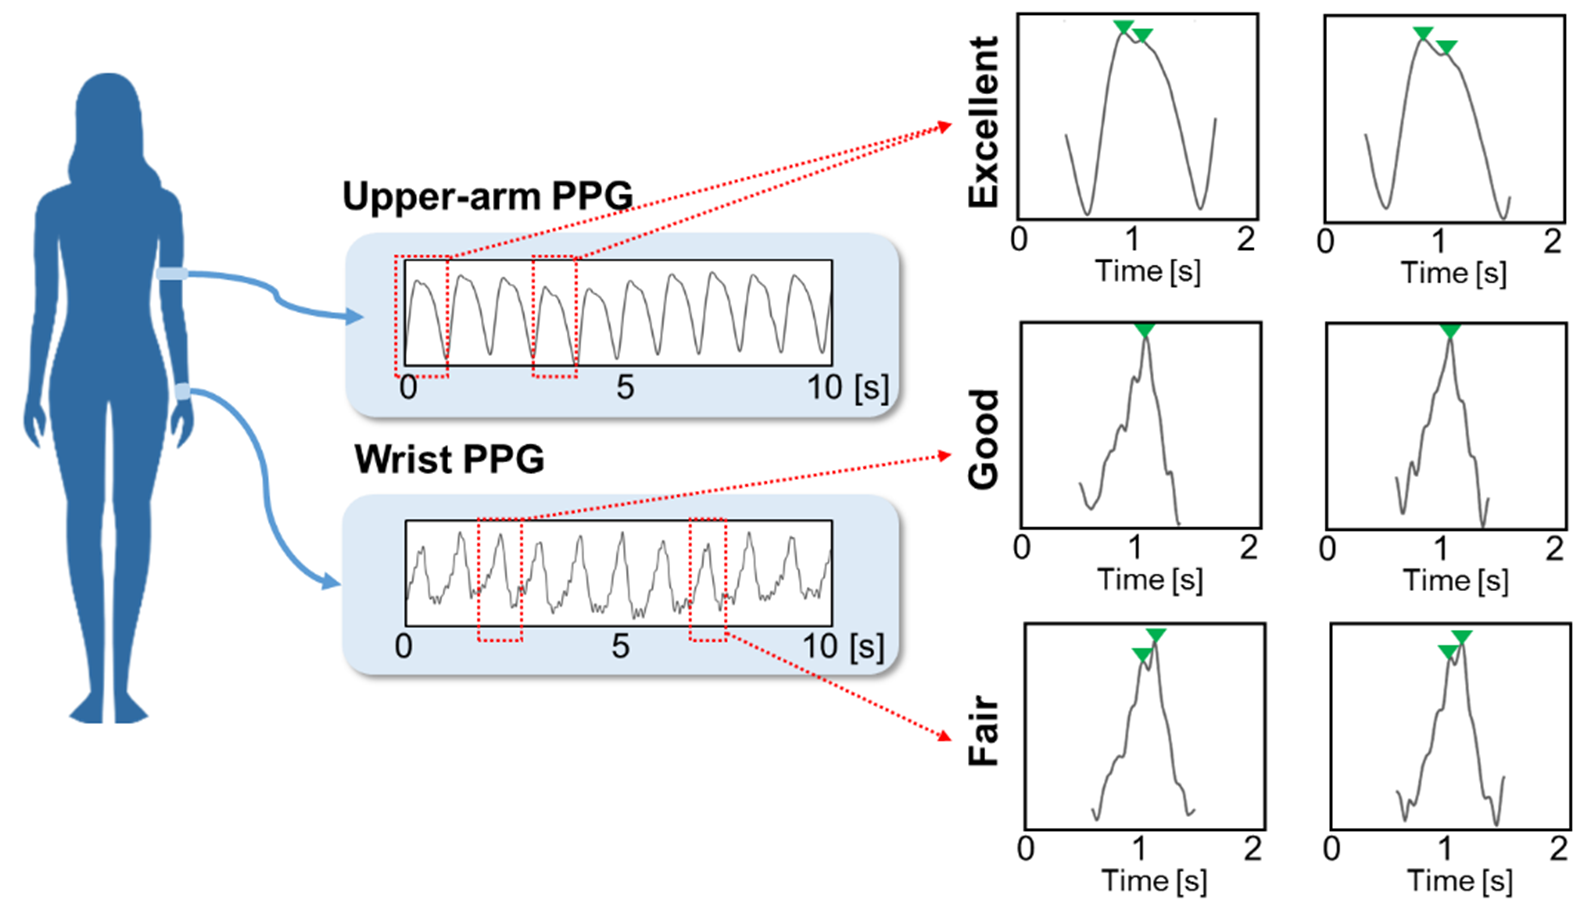
\includegraphics[width=0.6\textwidth]{CHPTRS/CH04_DISEÑO/imagenes/arm.png}
\caption{Comparación de señal entre brazo y muñeca}
\label{fig:comparaciúnUbicación}
\captionsetup{justification=centering,margin=1cm}
\caption*{\textit{Nota: Figura tomada de \cite{4.arm}}}
\end{figure}

\subsection{Señal del sensor}

Para obtener la frecuencia cardíaca, el sensor utiliza fotopletismografía. Esto consiste en que el sensor emite luz mediante un LED de cierto color, el cual cambia la distancia penetrada en la piel, y mide la luz reflejada por los tejidos con un fotodiodo, como se puede apreciar en la Figura~\ref{fig:ppg}. Esta luz reflejada varia en función de  los cambios en el volumen sanguíneo en los tejidos microvasculares de la piel \autocite{4.ppg}. 

\begin{figure}[H]
\centering
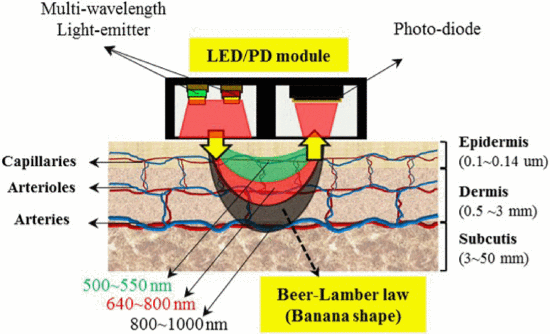
\includegraphics[width=0.7\textwidth]{CHPTRS/CH04_DISEÑO/imagenes/ppg.png}
\caption{Ilustración de medición de reflectancia con multiples colores de led}
\label{fig:ppg}
\captionsetup{justification=centering,margin=1cm}
\caption*{\textit{Nota: Figura tomada de \cite{4.ppgFOTO}}}
\end{figure}

\section{Diseño electrónico}
\subsection{Diagrama de bloques}
En la Figura~\ref{fig:4.diagramabBloques} se muestra el diagrama de bloques con las conexiones principales del sistema. El diagrama esta compuesto por 4 unidades principales: La unidad sensores que cuenta con el sensor MAX30102, encargado de obtener la frecuencia cardíaca del usuario y transmitirla mediante I2C. La unidad de actuadores, el cual consiste en un motor de vibración que es activado mediante una señal PWM. El microcontrolador responsable de la comunicación \textit{Bluetooth}, el procesamiento de las señales y la alimentación a la unidad de sensores y actuadores. Por ultimo, se tiene a la unidad de suministro de energía, el cual es el responsable de alimentar al microntroladro, asi como asegurar la autonomía energética del dispositivo. \\
 \begin{figure}[H]
    \centering
    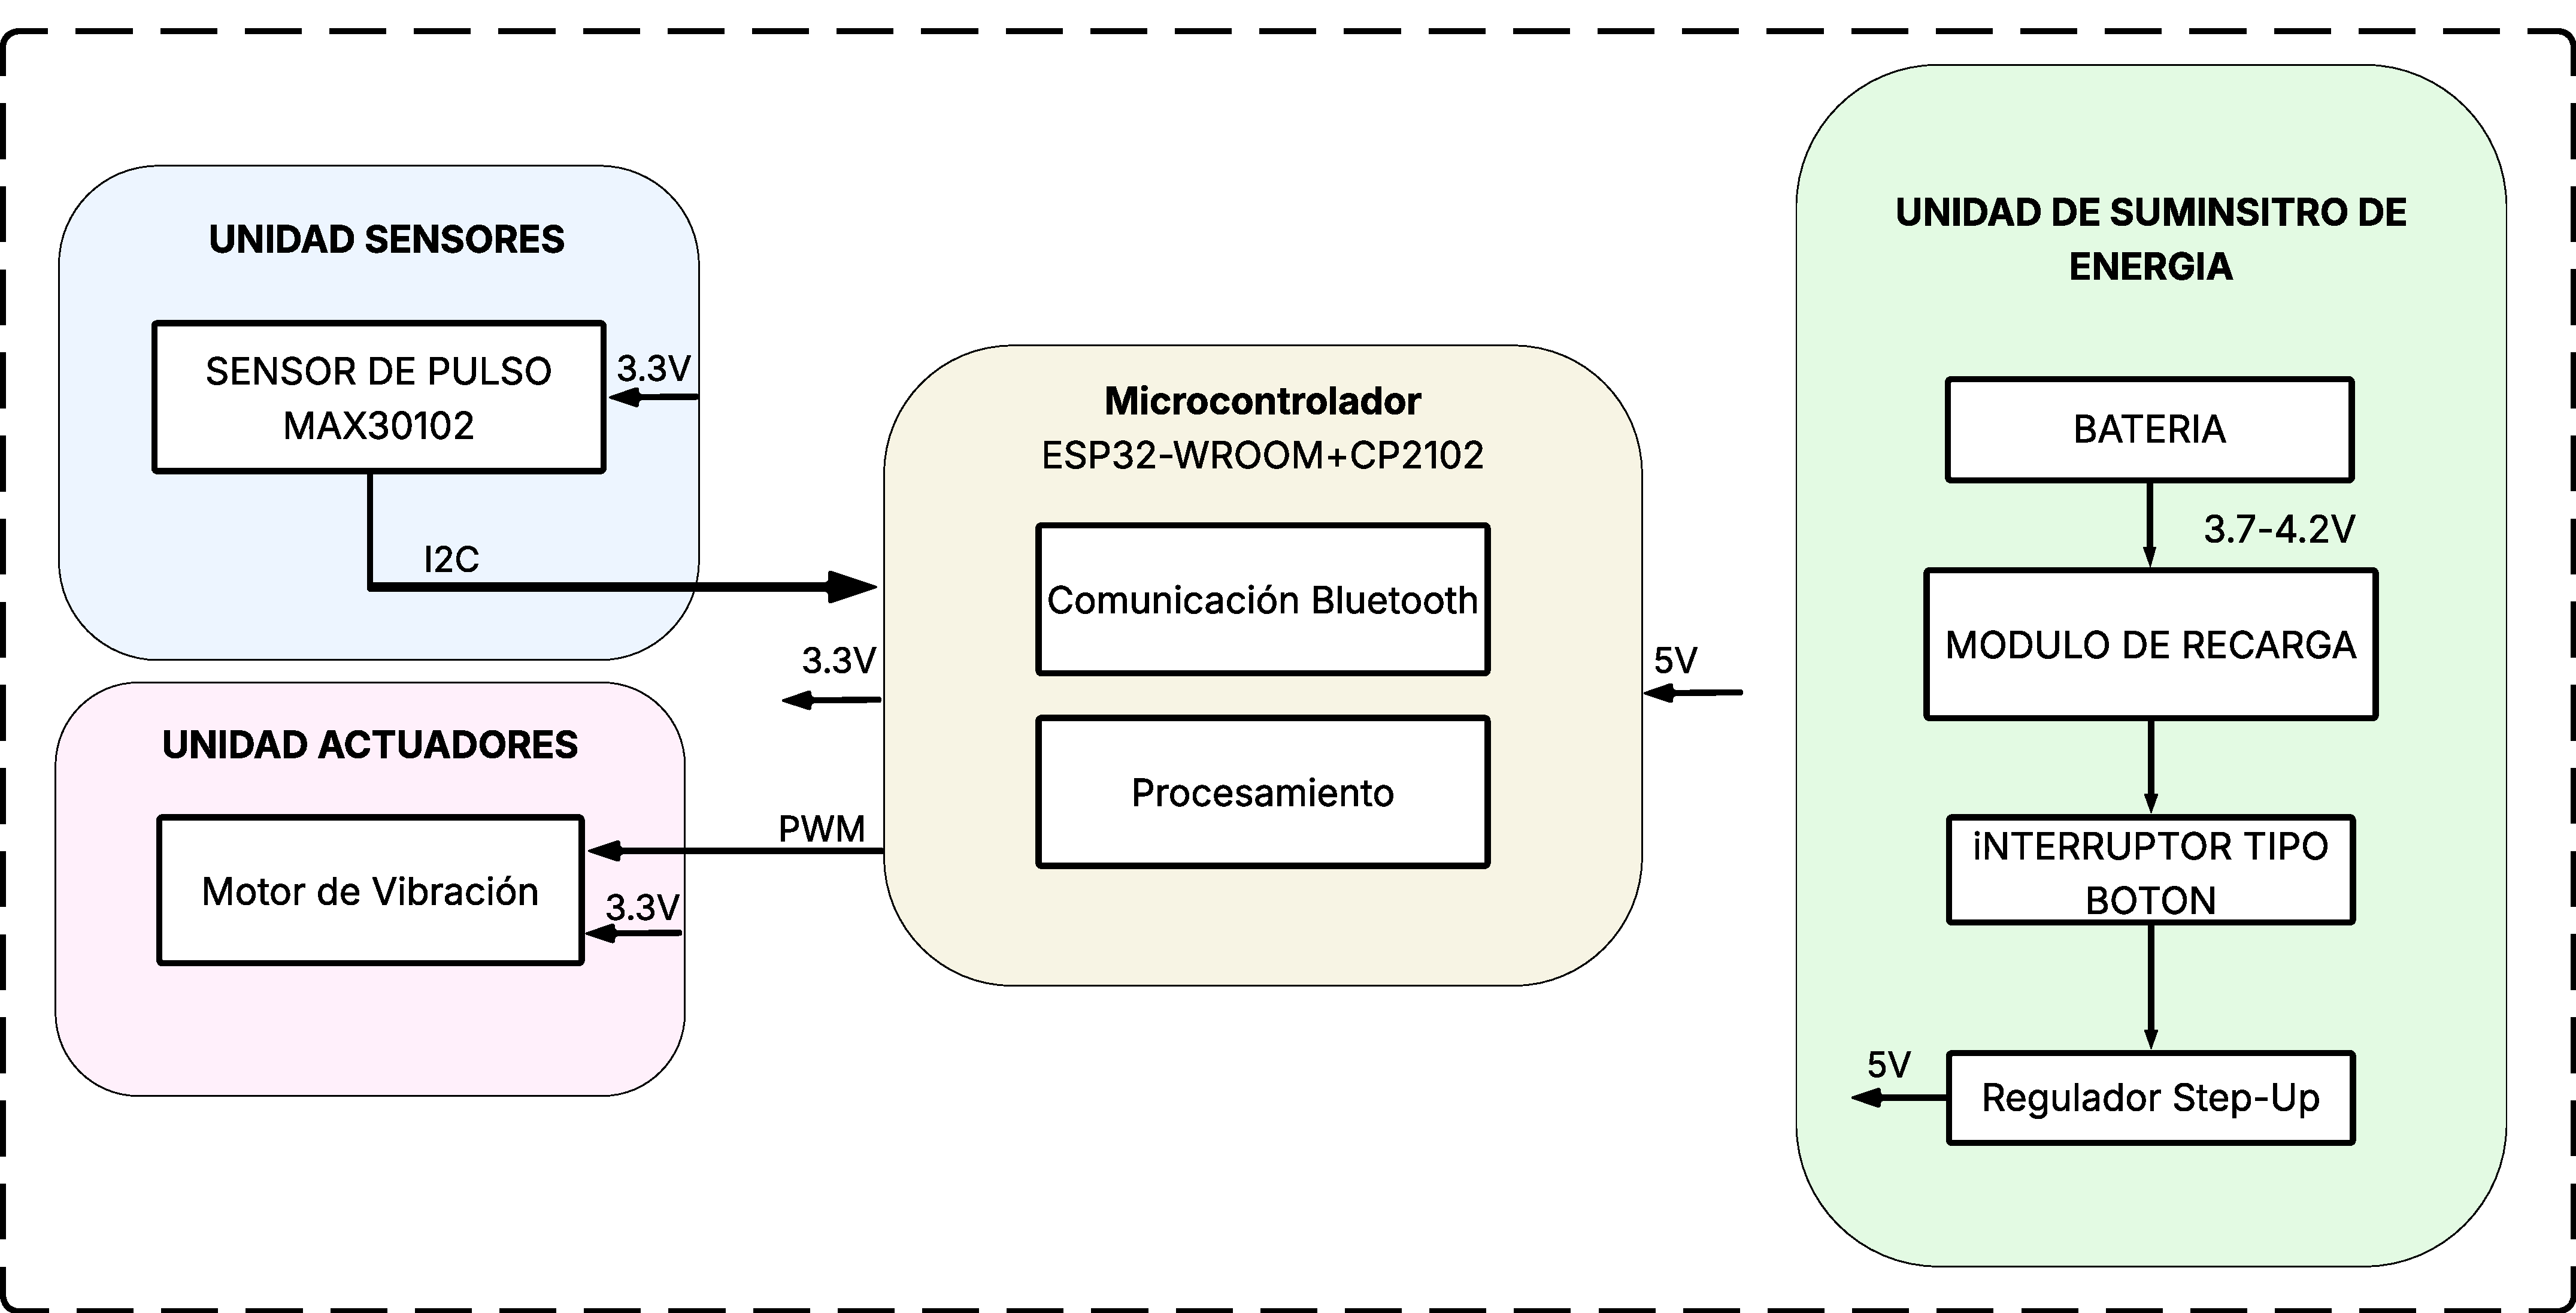
\includegraphics[width=0.8\textwidth]{CHPTRS/CH04_DISEÑO/imagenes/Diagrama de bloques.pdf}
    \caption{Diagrama de bloques}
    \label{fig:4.diagramabBloques}
    \captionsetup{justification=centering,margin=1cm}
   % \caption*{\textit{Nota: Figura tomada de \cite{4.motor}}}
    \end{figure}

\subsection{Microcontrolador}
    El microcontrolador es el encargado de realizar el control de todo el asistente, ya que en este estarán conectados el sensor MAX30102 y el motor de vibración. Por eso, el microcontrolador ha seleccionar debe contar con pines I2C que permitan la comunicación con el sensor mencionado previamente, pines PWM para el motor, así como la capacidad de realizar un procesamiento adecuado con una memoria mayor a 200KB ya que se contará con un clasificador, y la capacidad de comunicarse por \textit{Bluetooth} con el aplicativo.\\
    
    Por ello, el microcontrolador que se utilizará en esta tesis por motivos de estudio será el ESP-WROOM-32 como se ha mencionado previamente en la matriz morfológica (ver Tabla~\ref{tab:3.matrizcontrol}), integrado en un módulo que incluye el chip CP2102 (ver Figura ~\ref{fig:4.microcontrolador}) para la comunicación USB-Serial y la programación directa desde una computador. Este incorpora una conexión \textit{Bluetooth} v4.2 BR/EDR y BLE, así como WI-Fi. De esta manera se podrá enviar y recibir información del aplicativo móvil con la tecnología BLE \textit{(Bluetooth Low Energy)}, el cual destaca por un bajo consumo de corriente durante la comunicación inalámbrica, lo cual es importante para dispositivos portátiles como el asistente a desarrollar. Asimismo, presenta disponibilidad local, lo cual facilita su implementación a diferencia de las otras opciones para el presente trabajo. En la Tabla~\ref{tab:Tabla de características del microcontrolador} se muestran las características importantes del microcontrolador.
    
\begin{table}[H]
\centering


\begin{minipage}[t]{0.4\textwidth} % Imagen a la izquierda
    \centering
            \begin{figure}[H]

    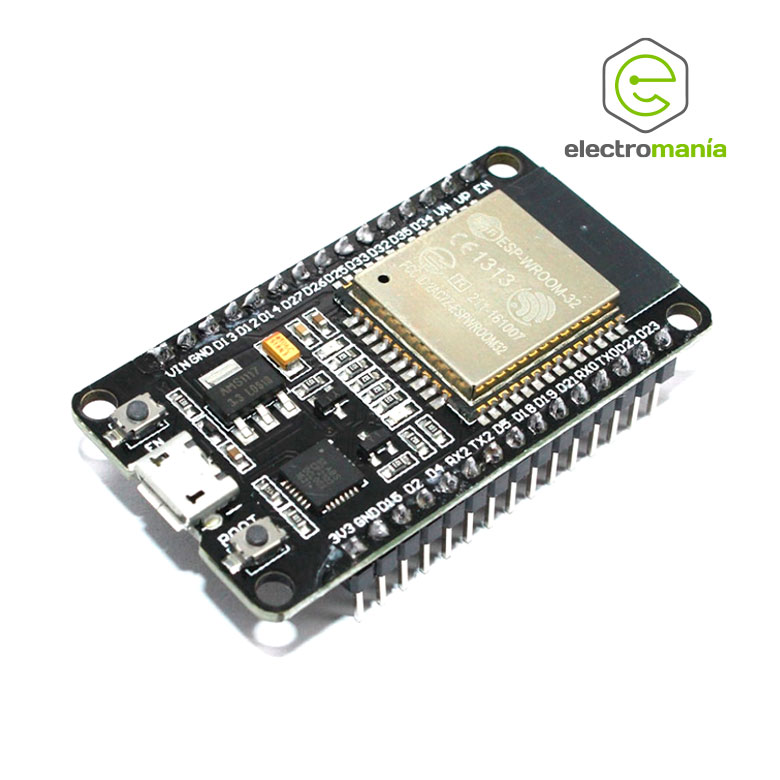
\includegraphics[width=0.8\linewidth]{CHPTRS/CH04_DISEÑO/imagenes/Micro_ESP32_Electromania-Peru.jpg}
    \captionof{figure}{Módulo ESP32-WROOM}
    \label{fig:4.microcontrolador}
    \captionsetup{justification=centering,margin=1cm}
    \caption*{\textit{Figura de \cite{4.ESP32}}}
            \end{figure}

\end{minipage}
\hfill
\begin{minipage}[t]{0.5\linewidth} % Tabla a la derecha
    \centering
    \caption{Características del microcontrolador ESP32-WROOM-32}
    \label{tab:Tabla de características del microcontrolador}
 \begin{table}[H]
    \centering
    \begin{tblr}{
        width = \linewidth,
        colspec = {X[c,m] X[c,m]},
        cells = {c},
        hlines,
        vlines
    }
    Característica & Valor \\
    Voltaje de alimentación              & 5 V                                      \\
    Corriente de consumo máxima          & 350 mA                                   \\
    Pines digitales                      & 25                                       \\
    Memoria del microcontrolador         & {Flash: 4 MB\\SRAM: 520 KB\\ROM: 448 KB} \\
    Frecuencia de reloj                  & 240 MHz                                  \\
    Corriente máxima por pin GPIO        & 40 mA                                   \\
    Dimensiones                          & 55 x 30 x 13 mm                           \\
    Peso                                 & 9 g
    \end{tblr}
      \end{table}
\end{minipage}

\end{table}

    
\subsection{Sensor de medición de frecuencia cardíaca}
En el caso del sensor de frecuencia cardíaca, se tiene que tener en cuenta que se busca utilizar aquellos que utilicen fotopletismografía (PPG). Por ello, en el mercado local se consideró los modelos MAX30102 y HW-827 (ver Figura~\ref{fig:4.MAX30102} y~\ref{fig:4.HW} respectivamente), cuyas características principales se encuentran en la Tabla~\ref{tab:TAbla comparacion sensores}. Sin embargo, si bien ambos son de bajo costo, se ha decidido emplear el sensor MAX30102 debido a que ofrece una mayor longitud de onda adecuada al utilizar un led infrarrojo a comparación del HW-827 que utiliza un led verde. Esta característica resulta fundamental para asegurar un sensado confiable en la zona braquial del asistente, donde existe mayor grosor de tejido, adecuado para el led infrarrojo, a comparación con el dedo, que es la ubicación más común para sensores basados en luz verde. Asimismo, el MAX30102 integra un filtro de luz ambiental (posible interferencia por fuentes externas de iluminación como luz solar o pantallas) , mejora la inmunidad al ruido externo y permite aplicar técnicas de filtrado digital que incrementan la calidad de la lectura sin la necesidad de circuitos adicionales.\\

\begin{table}[H]
\centering
\caption{Comparación de características de sensores PPG}
\label{tab:TAbla comparacion sensores}
\begin{tabular}{|c|c||c|c|} 
\hline
Características del sensor  & Requisitos mínimos & MAX30102                                                                                                    & HW-827                          \\ 
\hhline{|==::==|}
Voltaje de alimentación     & 3.3-5V             & 3.3-5 V                                                                                                     & 3.3-5V                          \\ 
\hline
Consumo máximo de corriente & menor a~ 40mA      & 20 mA                                                                                                       & 20mA                            \\ 
\hline
Leds integrados             & Rojo/infrarrojo    & \begin{tabular}[c]{@{}c@{}}Rojo (\textasciitilde{}660nm)\\Infrarrojo (\textasciitilde{}880 nm)\end{tabular} & Verde (\textasciitilde{}525nm)  \\ 
\hline
Señal                       & -                  & Digital                                                                                                     & Analógica                       \\ 
\hline
Dimensiones                 & Mínimas posibles   & 15 x 20 mm                                                                                                  & 15.8 Ø x 3.6 mm                 \\ 
\hline
Peso                        & Mínimo posibles    & 8g                                                                                                          & -                               \\
\hline
\end{tabular}
\end{table}


\begin{figure}[H]
    \centering
    % Primera imagen
    \begin{subfigure}{0.45\textwidth}
        \centering
        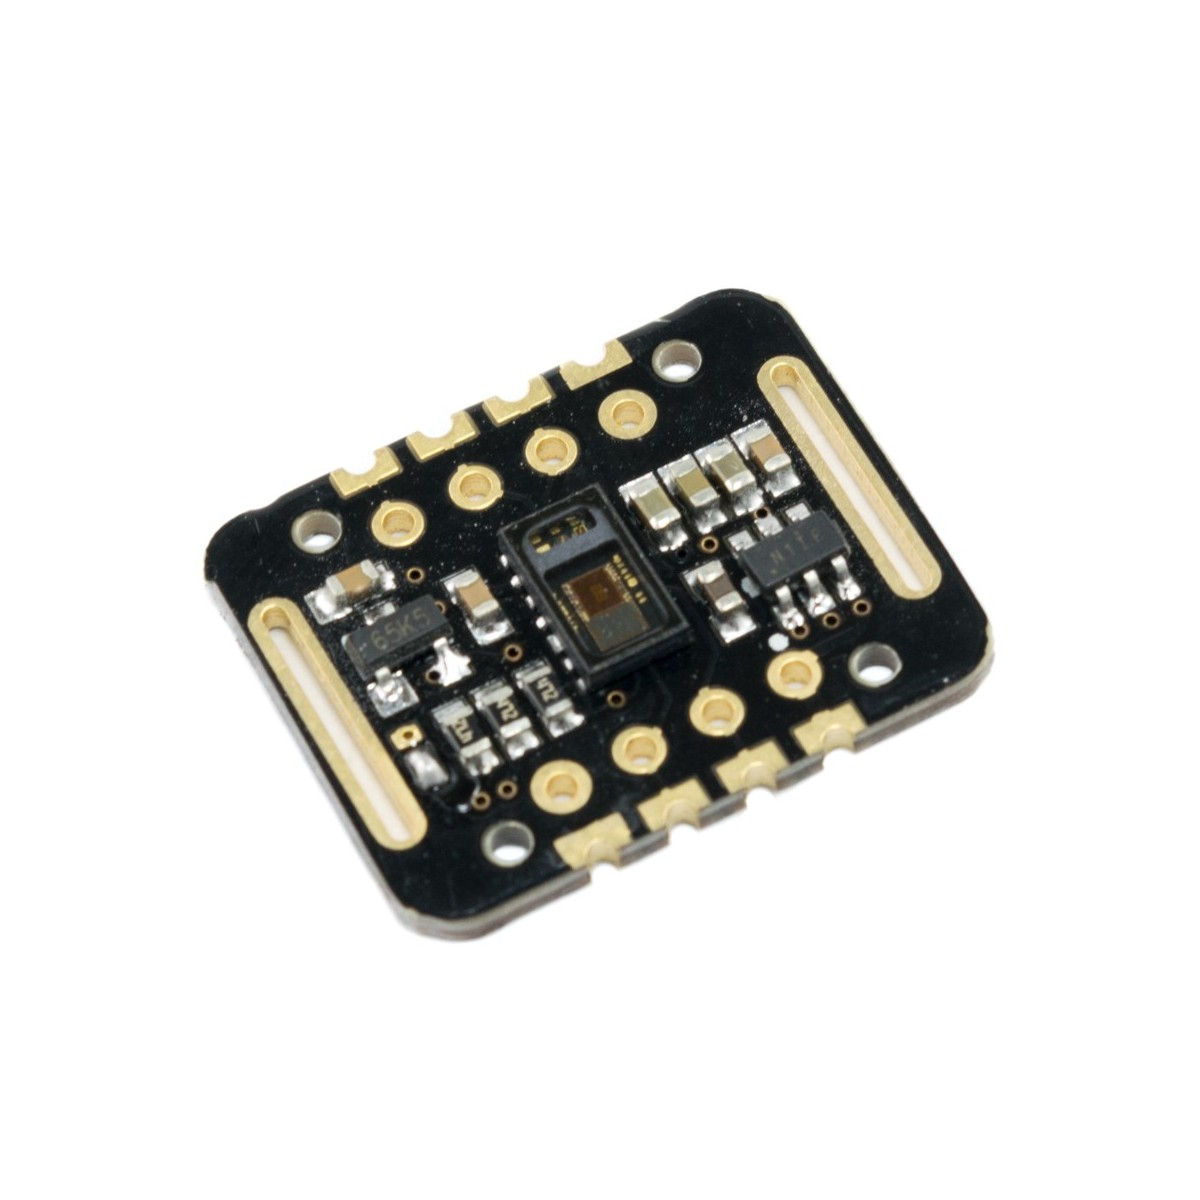
\includegraphics[width=\linewidth]{CHPTRS/CH04_DISEÑO/imagenes/MAX30102.png}
        \caption{Sensor MAX30102}
        \label{fig:4.MAX30102}
        \caption*{\textit{Figura tomada de \cite{4.max}}}
        
    \end{subfigure}
    \hfill
    % Segunda imagen
    \begin{subfigure}{0.45\textwidth}
       

        \centering
        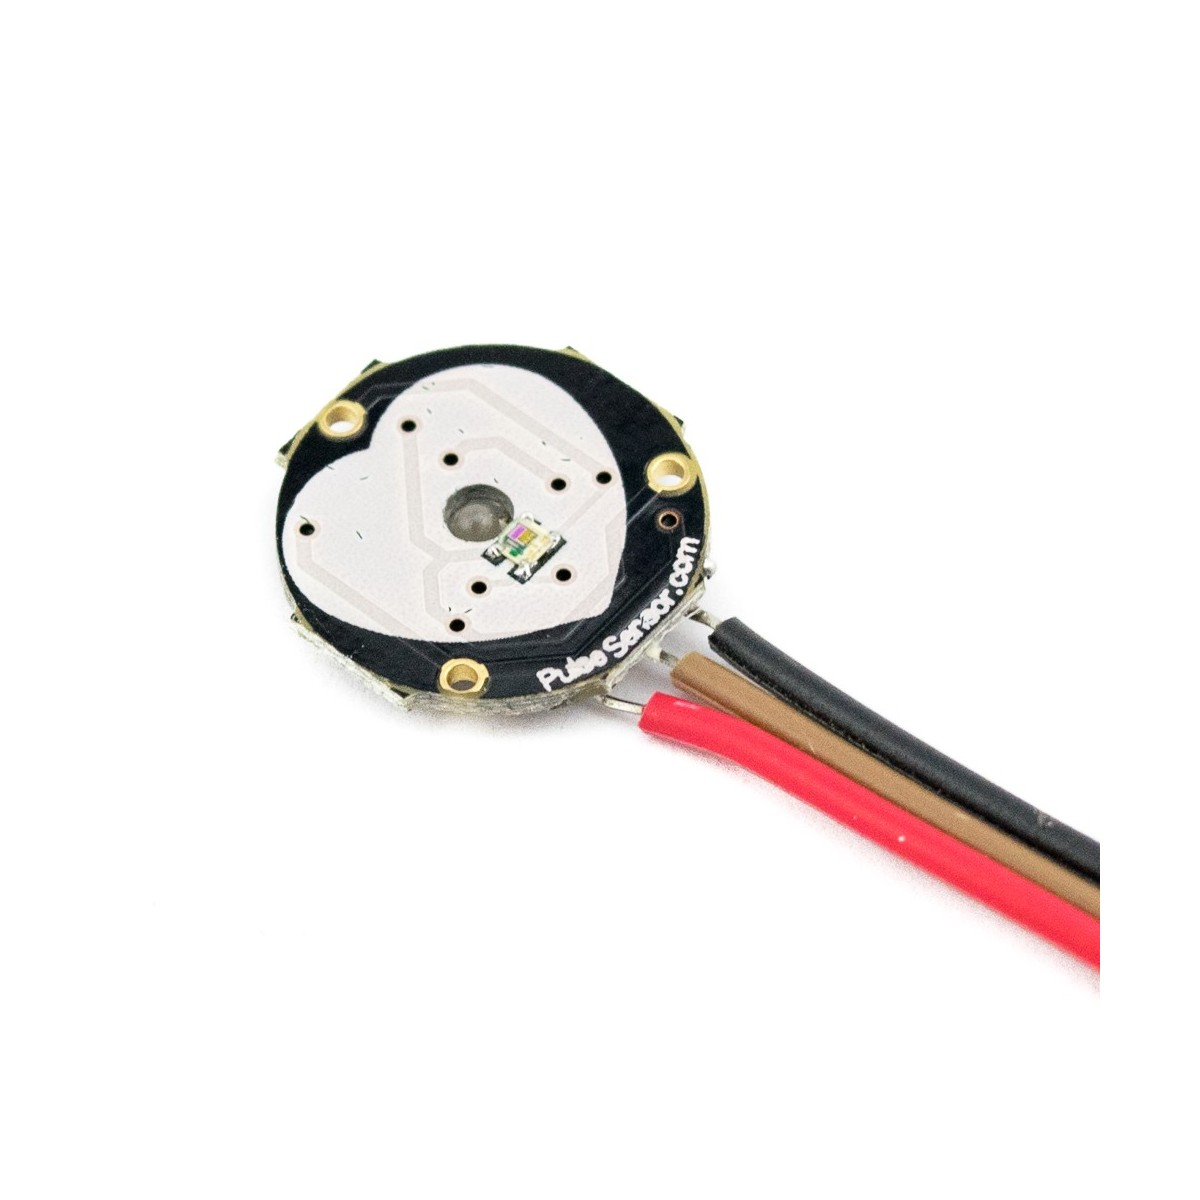
\includegraphics[width=\linewidth]{CHPTRS/CH04_DISEÑO/imagenes/SensorHW-827.png}
        \caption{Sensor HW-827}
        \label{fig:4.HW}
        \caption*{\textit{Figura tomada de \cite{4.hw-827}}}
        
    \end{subfigure}
    \caption{Sensores de frecuencia cardíaca considerados}
   
\end{figure}


\subsection{Motor de vibración}
El motor de vibración seleccionado, cuya función es brindar retroalimentación háptica, corresponde a un motor de masa giratoria excéntrica tipo moneda que se puede observar en la Figura~\ref{fig:4.motor moneda}, ya que este brinda una gran compatibilidad considerando que se necesita un tamaño compacto en el diseño propuesto de banda braquial a comparación del motor móvil y el motor cilíndrico (ver Figura~\ref{fig:4.motorB} y~\ref{fig:4.motorC} respectivamente), siendo este un factor determinante para la decisión final, ya que tienen características similares. Asimismo, cuenta con una tensión nominal baja, la corriente nominal media entre las opciones, alta disponibilidad y un  bajo costo, lo que lo convierte en una opción adecuada para el asistente.  En la siguiente Tabla~\ref{tab:4.Caracteristicas motor} se muestra la comparación entre las opciones de motores de vibración.

\begin{table}[H]
\centering
\caption{Comparación entre motores de vibración}
\label{tab:4.Caracteristicas motor}
\begin{tabular}{|c|c||c|c|c|} 
\hline
Características   & Requisitos       & Motor tipo moneda & Motor móvil & Motor cilíndrico  \\ 
\hhline{|==::===|}
Voltaje nominal   & 3-5V             & 3V                & 3V          & 1.5-3V            \\ 
\hline
Corriente nominal & Mínima posible   & 80mA              & 70mA        & 150mA             \\ 
\hline
Activación        & PWM              & PWM               & ~PWM        & PWM               \\ 
\hline
Dimensiones       & Mínimas posibles & 10Ø x 3 mm        & 16 x 6 mm   & 4Ø x 11.5 mm      \\ 
\hline
Peso              & Mínimo posible   & 1g                & -           & 6g                \\
\hline
\end{tabular}
\end{table}

 %  \begin{figure}[H]
  %  \centering
   % 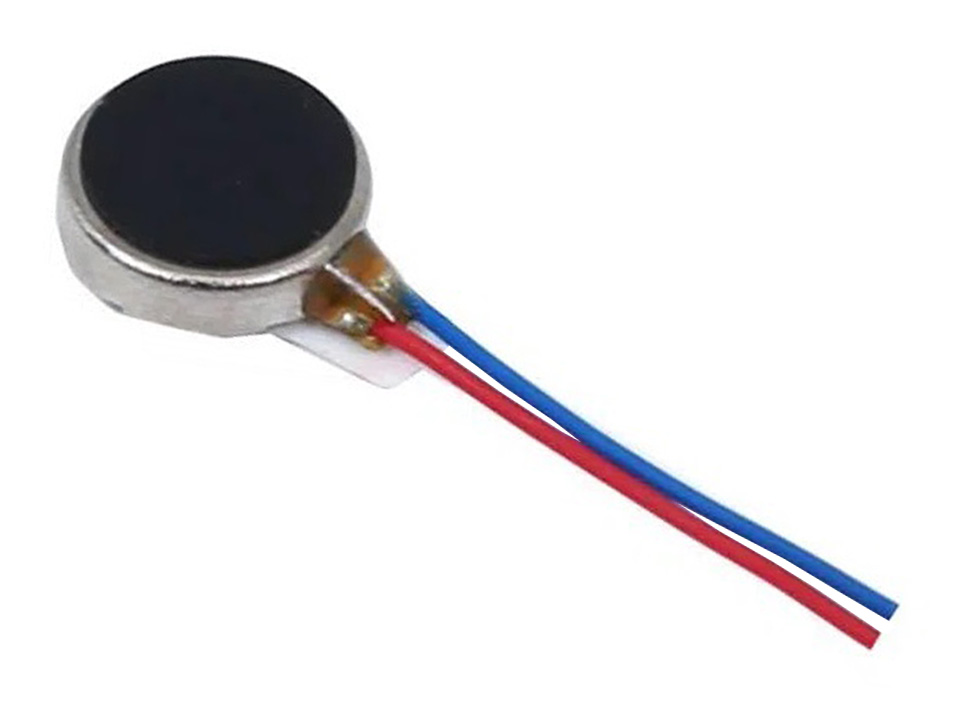
\includegraphics[width=0.4\textwidth]{CHPTRS/CH04_DISEÑO/imagenes/MotorERM.png}
    %\caption{Motor de vibración de masa giratoria excéntrica tipo moneda}
    %\label{fig:4.motor}
    %\captionsetup{justification=centering,margin=1cm}
    %\caption*{\textit{Nota: Figura tomada de \cite{4.motor}}}
    %\end{figure}

\begin{figure}[H]
    \centering
    % Primera imagen
    \begin{subfigure}{0.3\textwidth}
        \centering
        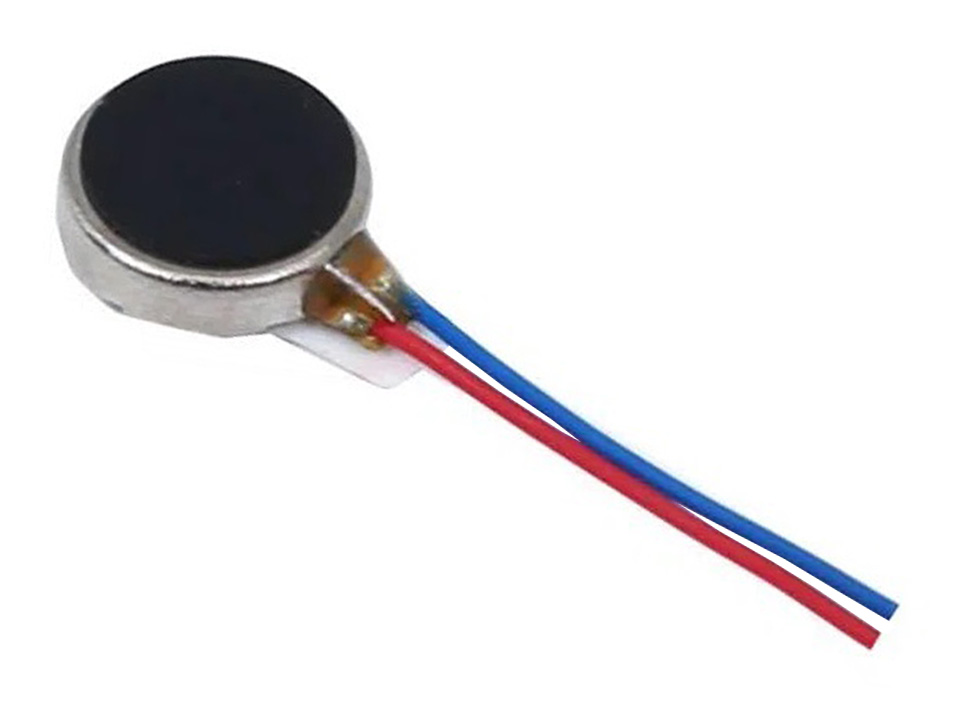
\includegraphics[width=\linewidth]{CHPTRS/CH04_DISEÑO/imagenes/MotorERM.png}
        \caption{Motor tipo moneda}
        \label{fig:4.motor moneda}
        \caption*{\textit{Figura tomada de \cite{4.motor}}}
        
    \end{subfigure}
    \hfill
    % Segunda imagen
    \begin{subfigure}{0.3\textwidth}
       

        \centering
        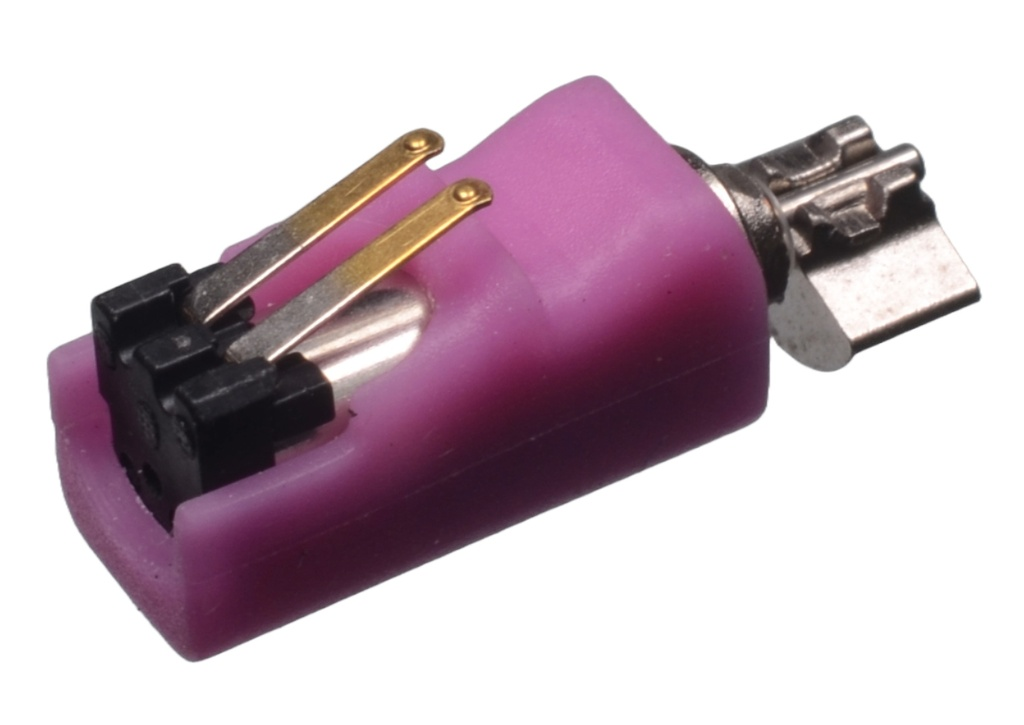
\includegraphics[width=\linewidth]{CHPTRS/CH04_DISEÑO/imagenes/Motor vib.png}
        \caption{Motor móvil}
        \label{fig:4.motorB}
        \caption*{\textit{Figura tomada de \cite{4.motorb}}}
        
    \end{subfigure}
     \hfill
    % Segunda imagen
    \begin{subfigure}{0.3\textwidth}
       

        \centering
        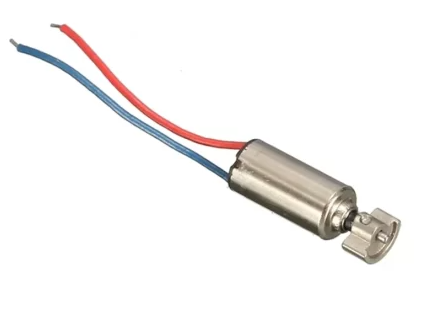
\includegraphics[width=\linewidth]{CHPTRS/CH04_DISEÑO/imagenes/Motor cilindrico.png}
        \caption{Motor cilíndrico}
        \label{fig:4.motorC}
        \caption*{\textit{Figura tomada de \cite{4.motorc}}}
        
    \end{subfigure}
    \caption{Motores de vibración considerados}
   
\end{figure}
    

Por otro lado, considerando que el motor estará conectado al microcontrolador y será activado mediante PWM, el ESP32 no puede suministrar corrientes altas por sus pines GPIO (máximo 40mA por pin). Por ello, es necesario realizar un circuito de protección o driver simple con un transistor NPN que permita proteger al microcontrolador y controlar al motor de manera segura (Figura~\ref{fig:4.motorproteccion}) y que no ocupe un tamaño considerable de espacio. Para ello, la base del transistor se conecta al pin PWM del microcontrolador mediante una resistencia que limita la corriente de base para proteger el GPIO. El transistor maneja la corriente del motor hacia tierra, mientras que se alimenta desde el pin 3.3V. Además, se coloca un diodo, en paralelo y polaridad opuesta al motor, para absorber los picos inducidos por el motor al apagarse, protegiendo al transistor y al resto del circuito.\\


    \begin{figure}[H]
    \centering
    % Primera imagen
    \begin{subfigure}{0.45\textwidth}
        \centering
        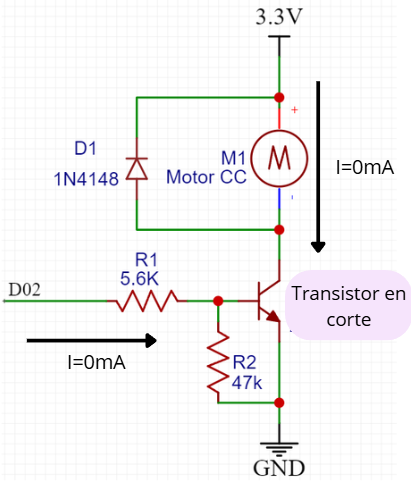
\includegraphics[width=\linewidth]{CHPTRS/CH04_DISEÑO/imagenes/corte.png}
        \caption{Corrientes con transistor en corte}
        
    \end{subfigure}
    \hfill
    % Segunda imagen
    \begin{subfigure}{0.48\textwidth}
       

        \centering
        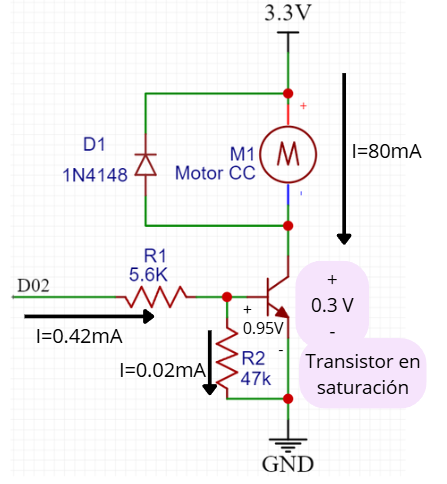
\includegraphics[width=\linewidth]{CHPTRS/CH04_DISEÑO/imagenes/sat.png}
        \caption{Corrientes con transistor en saturación}
        
        
        
    \end{subfigure}
     
    % Segunda imagen
    
    \caption{Circuito de protección del motor}
    \label{fig:4.motorproteccion}
   
\end{figure}

El transistor seleccionado es el 2N3904 que cuenta con una $V_{CE(sat)}$ de 0.3V, una ganancia $h_{FE}$ de 200 en promedio, un $V_{BE(sat)}$ de 0.95V maximo según su hoja de datos. Asimismo, como se sabe que la corriente del conector($I_C$) es 80mA por parte del motor y utilizando la relación $I_C=h_{FE}\,I_B$, con $h_{FE} = 200$ se obtiene que la corriente de la base ($I_{B0}$) es igual a 0.4mA. Adicionalmente, conocienco  el voltaje que es emitido desde el microcontrolador es de 3.3V, se utiliza la Ecuación~\ref{ec:4.motor} para hallar el valor de la resistencia R1 que es de $5.875\,k\Omega$, eligiendo el valor comercial más próximo de $5.6\,k\Omega$.
\begin{align}
\label{ec:4.motor}
R1=\frac{V_{GPIO}-V_{BE(sat)}}{I_{B0}}\,\,\,\text{[\si{\ohm}]}
\end{align}

Adicionalmente, al colocar $R1 = 5.6\,k\text{\si{\ohm}}$, se obtiene una corriente $I_{B}$ distinta a la calculada previamente. Esta se halla mediante la Ecuación~\ref{ec:4.motorcorrientIB}, obteniendo como resultado $I_{B1} = 0.42\,\si{\milli\ampere}$
\begin{align}
\label{ec:4.motorcorrientIB}
I_B=\frac{V_{GPIO}-V_{BE(sat)}}{R1}\,\,\,\text{[\si{\ampere}]}
\end{align}

Finalmente, se ha colocado la resistencia $R2 = 47\,k\text{\si{\ohm}}$ de protección, para asegurar la llegada de solo $0.4\, \si{\milli\ampere}$ al transistor, la cual es una corriente muy por debajo de los 40mA permitidos por el GPIO del ESP32. Esta resistencia es colocada en paralelo a Base-Emisor, obtenido mediante la Ecuación~\ref{ec:4.motorR2}.
\begin{align}
\label{ec:4.motorR2}
R2=\frac{V_{BE}}{I_{B1}-I_{B0}}\,\,\,\text{[\si{\ohm}]}
\end{align}

\subsection{Módulo de carga}
En el caso del módulo de carga, los requisitos son que pueda recargar baterías de litio, se pueda conectar mediante una entrada Tipo C y que tenga las dimensiones más pequeñas posible. Por eso, el módulo de carga que se va a utilizar será el HW-373 que es puede apreciar en la Figura~\ref{fig:4.carga}, el cual esta basado en el chip TP4056. Este módulo permite la recarga de  baterías de litio mediante una entrada USB tipo C, lo cual aporta compatibilidad con cargadores modernos. Asimismo, contiene protección contra sobretensión, sobrecorriente, sobretemperatura y cortocircuitos, lo cual permite garantizar la seguridad de la batería y del sistema eléctrico durante el proceso de carga. Su alta disponibilidad, reducido tamaño y costo lo convierten en una opción confiable para aplicaciones portátiles como el del asistente. La siguiente Tabla~\ref{tab:4.Caracteristicas modulo de carga} muestra las características más importantes del módulo HW-373.

\begin{figure}[H]
\centering
\begin{minipage}[t]{0.55\textwidth}
\vspace{0pt} % <-- asegura alineación real
\centering
\captionof{table}{Características principales del módulo de carga HW-373}
\label{tab:4.Caracteristicas modulo de carga}

\begin{tblr}{
  width = \linewidth,
  colspec = {X[c,m] X[c,m]},
  cells = {c},
  cell{1}{1} = {c=2}{0.931\linewidth},
  hlines,
  vlines,
}
Características del módulo de carga             &                                         \\
Voltaje de entrada (Tipo C)                    & 5V                                      \\
Corriente de protección contra sobre corriente & 3A                                      \\
Corriente de carga ajustable                   & 1A                                      \\
Peso                                           & 2g                                      \\
Indicadores                                    & {Rojo - Cargando\\Azul - Carga completa} \\
Temperatura de funcionamiento                  & -40°C a +85°C                           \\
Dimensiones                                    & 27.7 x 17 mm                            \\
\end{tblr}
\end{minipage}
\hfill
\begin{minipage}[t]{0.40\textwidth}
\vspace{0pt} % <-- asegura alineación real
\centering
\rotatebox{90}{
  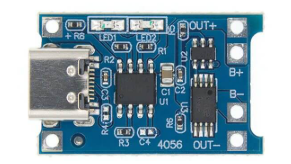
\includegraphics[width=\linewidth]{CHPTRS/CH04_DISEÑO/imagenes/Modulo de carga.png}
}
\caption{Módulo de carga HW-373}
\label{fig:4.carga}
\caption*{\textit{Nota: Figura de \cite{4.carga}}}
\end{minipage}
\end{figure}


 \subsection{Regulador de voltaje}
 Para seleccionar los reguladores de voltaje es necesario saber la corriente de consumo del asistente. En la Tabla~\ref{tab:4.Consumo corrientes} se muestra la potencia de consumo de los componentes del circuito electrónico. A través de estos datos se podrá determinar el regulador de voltaje \textit{Step-Up} para el microcontrolador y el regulador \textit{Step-Down} para el motor y sensor
 
\begin{table}[H]
\centering
\caption{Consumo de potencia  del circuito electrónico}
\label{tab:4.Consumo corrientes}
\begin{tblr}{
  column{1} = {c},
  column{2} = {c},
  cell{5}{1} = {c=3}{},
  hlines,
  vlines,
}
Componente         & Corriente de uso & Voltaje & Potencia \\
Módulo ESP32 (BLE) & 100 mA~          & ~5 V    & 500 mW   \\
Sensor MAX30101    & 20mA             & 3.3 V   & 66mW     \\
Motor de vibración & 80mA             & 3.3 V   & 264mW    \\
Total              &                  &         & 830mW    
\end{tblr}
\end{table}

El voltaje que las baterías recargables portables brindan es de 3.7 V; sin embargo, el microcontrolador opera a 5 V. Por ello, se requiere un elevador de voltaje y se optó por un \textit{Step Up} modelo MT3608 (ver Figura~\ref{fig:4.regulador}) debido a su disponibilidad en el mercado local y cumple con el requisito básico, de aumentar a 5 voltios, el voltaje de 3.7 voltios que suelen brindar las baterías para poder alimentar el microcontrolador por la entrada Vin y una corriente de salida máxima de 2 A. Sin embargo, se debe recalcar que existen opciones más compactas, como los de la serie U3V40x de Pololu, que permitirían optimizar mejor el tamaño y por ende aumentar la portabilidad. No obstante, estos son de elevado costo y de baja disponibilidad local. Por lo tanto, dentro del trabajo de esta tesis se optó por utilizar el MT3608 como solución práctica, sus principales características se encuentran en la  Tabla~\ref{tab:4.Caracteristicas regulador}.

 



\begin{table}[H]
\centering
\caption{Características de los reguladores Step-Up}
\label{tab:4.Caracteristicas regulador}
\begin{tabular}{|c|c||c|c|} 
\hline
Características del regulador  & Requisitos       & MT3608         & U3V40F5                \\ 
\hhline{|==::==|}
Voltaje de Entrada             & 3.7V             & 2V a 24V~      & 1.3-5V                 \\ 
\hline
Voltaje de Salida              & 5V               & 5V a 28V       & 5V                     \\ 
\hline
Corriente de salida            & min 200mA        & 2A             & 9.5A                   \\ 
\hline
Protección sobre - temperatura & -                & SI             & -                      \\ 
\hline
Eficiencia de conversión       & min 90\%         & 93\% máx.      & 94 \% Max              \\ 
\hline
Peso                           & Mínimo posible   & 5g             & 1.5g                   \\ 
\hline
Dimensiones                    & Mínimas posibles & 36 x 17 x 7 mm & 15.4 x 15.4 x 5.59 mm  \\
\hline
\end{tabular}
\end{table}


\begin{figure}[H]
    \centering
    % Primera imagen
    \begin{subfigure}{0.4\textwidth}
        \centering
        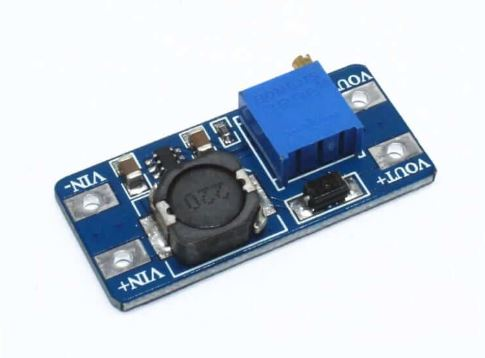
\includegraphics[width=\linewidth]{CHPTRS/CH04_DISEÑO/imagenes/regulador.png}
        \caption{Regulador MT3608}
        \label{fig:4.regulador}
        \caption*{\textit{Figura tomada de \cite{4.regulador}}}
        
    \end{subfigure}
    \hfill
    % Segunda imagen
    \begin{subfigure}{0.4\textwidth}
       

        \centering
        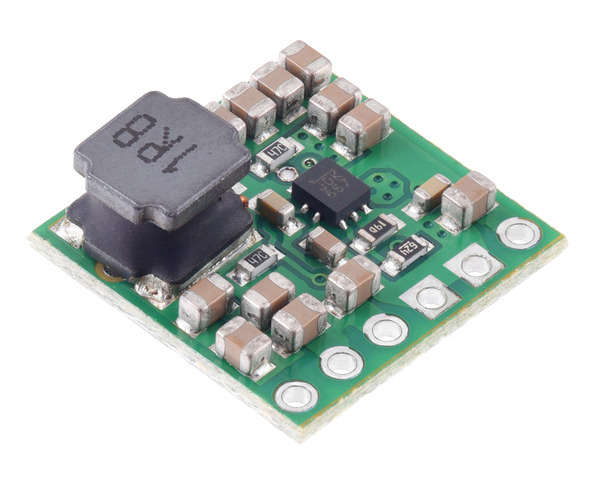
\includegraphics[width=\linewidth]{CHPTRS/CH04_DISEÑO/imagenes/reguladorUP2.png}
        \caption{Regulador U3V40F5}
        \label{fig:4.pololu}
        \caption*{\textit{Figura tomada de \cite{4.pololu}}}
        
    \end{subfigure}
    \caption{Reguladores \textit{Step-Up} considerados}

\end{figure}

Asimismo, sabemos que el sensor MAX30102 y el motor de vibración seleccionados operan a un voltaje de 3.3 V a 20mA y 80mA respectivamente. Por ello, se ha seleccionado un regulador \textit{Step Down} modelo MP1584 (Figura~\ref{fig:4.mp}) debido a que cumple con el requisito básico de diminuir los 5V a un 3.3 V, unas dimensiones ligeramente más pequeñas como se observa en la Tabla~\ref{tab:4.Caracteristicas regulador step-dopwn} y una mayor eficiencia que el módulo AMS (Figura~\ref{fig:4.ams}), ya que este último es un regulador lineal.

\begin{table}[H]
\centering
\caption{Características de los reguladores Step-Down}
\label{tab:4.Caracteristicas regulador step-dopwn}
\begin{tabular}{|c|c||c|c|} 
\hline
Características del regulador & Requisitos       & MP1584         & AMS1117          \\ 
\hhline{|==::==|}
Voltaje de Entrada            & 3.7V             & 4.5 a 28V      & 4-12V            \\ 
\hline
Voltaje de Salida             & 5V               & 0.8 a 18V      & 3.3V             \\ 
\hline
Corriente de salida           & min 200mA        & 3A             & 800 mA           \\ 
\hline
Eficiencia de conversión      & Máxima posible   & 96\% máx.      & 66\%             \\ 
\hline
Peso                          & Mínimo posible   & 3g             & 1.5g             \\ 
\hline
Dimensiones                   & Mínimas posibles & 22 x 17 x 4 mm & 36 x 17 x 14 mm  \\
\hline
\end{tabular}
\end{table}
\begin{figure}[H]
    \centering
    % Primera imagen
    \begin{subfigure}{0.4\textwidth}
        \centering
        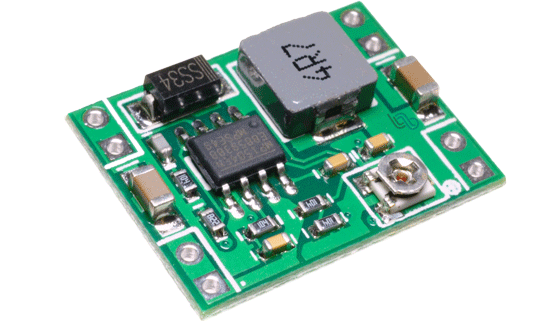
\includegraphics[width=\linewidth]{CHPTRS/CH04_DISEÑO/imagenes/MP15.png}
        \caption{Regulador MP1584}
        \label{fig:4.mp}
        \caption*{\textit{Figura tomada de \cite{4.regulador}}}
        
    \end{subfigure}
    \hfill
    % Segunda imagen
    \begin{subfigure}{0.32\textwidth}
       

        \centering
        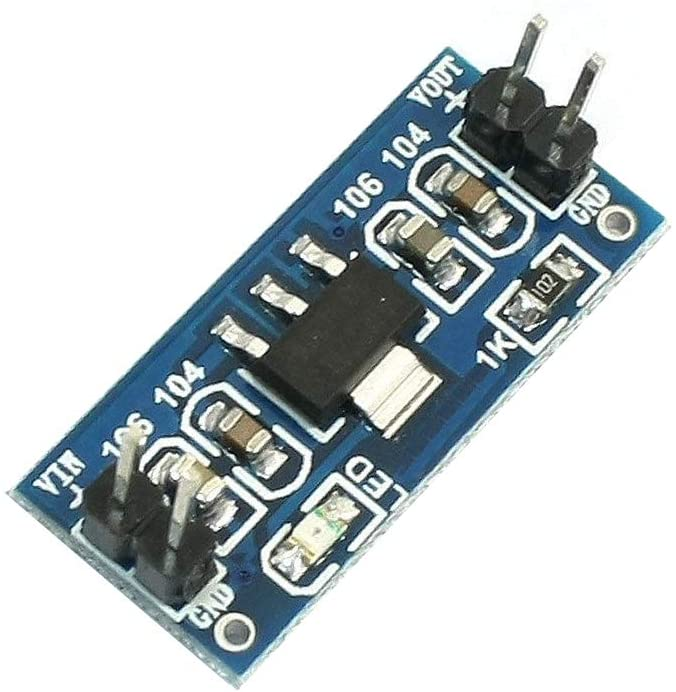
\includegraphics[width=\linewidth]{CHPTRS/CH04_DISEÑO/imagenes/ams.png}
        \caption{Regulador AMS1117}
        \label{fig:4.ams}
        \caption*{\textit{Figura tomada de \cite{4.pololu}}}
        
    \end{subfigure}
    \caption{Reguladores \textit{Step-Down} considerados}

\end{figure}
En la Figura~\ref{fig:4.eficiencia} se muestra la gráfica Eficiencia vs Corriente de salida extraída de la hoja de datos del regulador \textit{Step-Up} seleccionado. Esta  permite tener como referencia una eficiencia aproximada de 92\% para una entrada de 3.7V y una salida de 5V. Asimismo, si bien en la Tabla~\ref{tab:4.Consumo corrientes} se muestra un consumo máximo de 200 mA, se tiene que tener en cuenta que el motor no se encontrará siempre encendido, ya que se busca que este solo se active en caso de retroalimentación con una duración entre 200 y 500 milisegundos. Por ello, se optó por hacer el cálculo de corriente necesaria en la batería, considerando ambos casos: 120 mA sin motor y 200 mA con motor.
\begin{figure}[H]
    \centering
    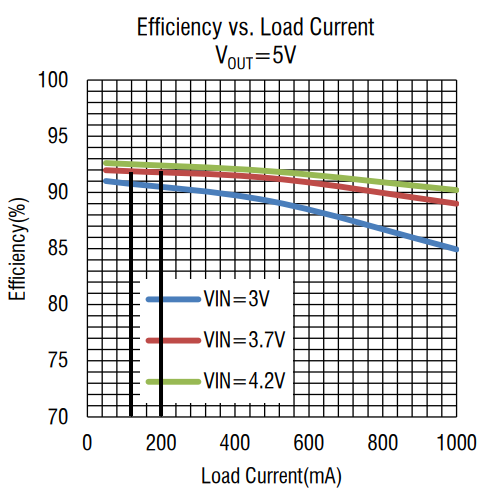
\includegraphics[width=0.45\textwidth]{CHPTRS/CH04_DISEÑO/imagenes/Eficiencia.png}
    \caption{Curva Eficiencia vs Corriente de salida del MT3608}
    \label{fig:4.eficiencia}
    \captionsetup{justification=centering,margin=1cm}
    \caption*{\textit{Nota: Figura tomada de \cite{4.eficiencia}}}
    \end{figure}

De igual manera, en la Figura~\ref{fig:4.eficiencia33} se muestra la gráfica Eficiencia vs Corriente de salida del regulador \textit{Step-Down} seleccionado, donde si bien no se muestra la curva para una entrada de 5V. Por ello, a través de aproximaciones, permite tener una referencia aproximada de 85\%Además, la corriente de entrada de cada regulador se calcula en base la Ecuación~\ref{ec:4.regu}.
\begin{align}
\label{ec:4.regu}
I_{IN} &= \frac{I_{OUT}* V_{OUT}}{Eficiencia* V_{IN}} 
\end{align}

donde $I_{IN}$ e $I_{OUT}$  son las corrientes de entrada y salida del regulador, y $V_{IN}$ y $V_{OUT}$  son también los voltajes de entrada y salida del regulador. En el caso del regulador MP1584 se tiene como corriente de salida los 20mA del sensor en el primer caso, con un voltaje de salida 3.3V y un voltajde entrada de 5V y una eficiencia de 85\%, dando como resultado que la corriente de entrada para este regulador $I_{INSD_1} =15.53 mA$. Para el segundo caso, donde se consideran los 80 mA del motor, se obtiene$I_{INSD_2} =77.65 mA$ A partir de esta, se obtiene la corriente de salida para el regulador \textit{Step-Up} a través de la Ecuación~\ref{ec:4.regu5}.
\begin{align}
\label{ec:4.regu5}
I_{outSU} &= I_{ESP}+ I_{INSD} 
\end{align}

donde $I_{ESP}$ es 100mA y $I_{INSD}$ corresponde a los 15.53mA y 77.65 mA calculados previamente para caso, obteniendo una corriente de salida total de 115.53mA para el primer caso y 177.65mA para el segundo caso, reemplazando con los valores correspondientes para este regulador, se tiene que se necesita una corriente de entrada $I_{tot_1}=169.69mA$ para el primer caso y $I_{tot_2}=260.94mA$ para el segundo caso. A partir de este valor se puede seleccionar la batería adecuada para el asistente.


\begin{figure}[H]
    \centering
    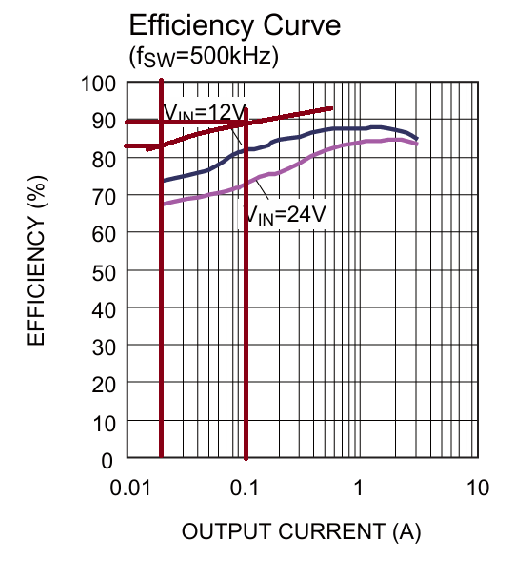
\includegraphics[width=0.4\textwidth]{CHPTRS/CH04_DISEÑO/imagenes/Eficiencia33.png}
    \caption{Curva Eficiencia vs Corriente de salida del MP1584}
    \label{fig:4.eficiencia33}
    \captionsetup{justification=centering,margin=1cm}
    \caption*{\textit{Nota: Figura tomada de \cite{4.eficiencia}}}
    \end{figure}
    
\subsection{Batería del dispositivo}

La batería utilizada en el asistente es de Litio, las cuales poseen un voltaje nominal de 3.7 V. Asimismo, considerando que se requiere una autonomía energética que pueda abarcar sesiones de estudio de al menos 4 horas como mínimo, se calcula la capacidad $Cap$ que debe tener la batería seleccionada con la Ecuación~\ref{ec:4.cap}.
\begin{align}
\label{ec:4.cap}
Cap=I_{tot}*h
\end{align}

donde $I_{tot}$ corresponde a la corriente calculadas previamente para cada caso ($I_{tot_1}=169.69mA$ y $I_{tot_2}=260.94mA$ ) y $h$ son las horas requeridas del funcionamiento del sistema. Al reemplazar los valores mencionados se obtiene una capacidades de  678.76 mAh y 1043.76mAh. Al observar estos resultados, es necesario optimizar el uso del motor unicamente en los casos de distracción con un tiempo de funcionamiento en el rango mencionado previamente.\\

Al implementar un factor de seguridad de 1.3 considerando que las baterías pueden descargarse hasta un 80\% para no dañarse, se requieren 877,65mAh y 1356,88mAh. Sin embargo, se optó por una batería de 1000 mAh (ver Figura~\ref{fig:4.bateria}), ya que se busca que el motor este en funcionamiento por tiempos muy cortos de retroalimentación. Además, permite conseguir una duración de 5.92 horas aproximadamente en el primer caso, es comercial y tiene un tamaño compacto.

\begin{figure}[H]
    \centering
    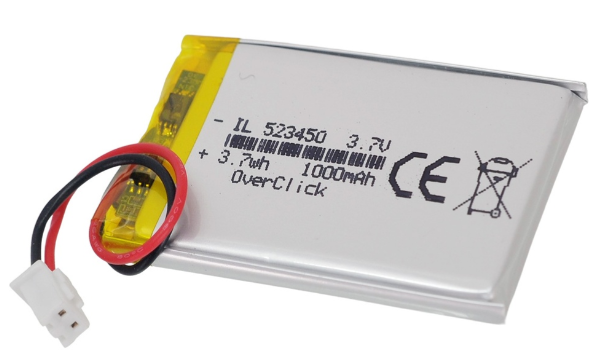
\includegraphics[width=0.6\textwidth]{CHPTRS/CH04_DISEÑO/imagenes/bateria.png}
    \caption{Batería recargable de Litio 1000 mAh}
    \label{fig:4.bateria}
    \captionsetup{justification=centering,margin=1cm}
    \caption*{\textit{Nota: Figura tomada de \cite{4.bateria}}}
    \end{figure}

\subsection{Switch de encendido}
El switch que se ha decidido emplear en el presente trabajo es uno de tipo botón que cuenta con enganche (ver Figura~\ref{fig:4.boton}), ya que este permitirá con facilidad que el usuario pueda identificar cuando esta encendido y cuando apagado. Asimismo, cuenta con una alta disponibilidad adecuada, es compacto y sus características facilitan su integración, ya que este soporta una corriente de 0.3 amperios a 30 voltios. 

\begin{figure}[H]
    \centering
    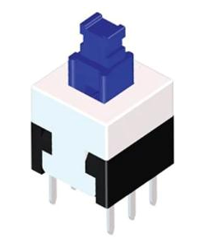
\includegraphics[width=0.25\textwidth]{CHPTRS/CH04_DISEÑO/imagenes/boton.png}
    \caption{Switch tipo botón}
    \label{fig:4.boton}
    \captionsetup{justification=centering,margin=1cm}
    \caption*{\textit{Nota: Figura tomada de \cite{4.boton}}}
    \end{figure}


\subsection{Diagrama esquemático}
En la Figura~\ref{fig:4.esquematico} se muestra el diagrama esquemático general del sistema. El microcontrolador ESP32 es alimentado por el regulador step up. Asimismo, el regulador step down es el encargado de alimentar al sensor MAX30102 y al motor de vibración con 3.3 V. 
\begin{figure}[H]
    \centering
    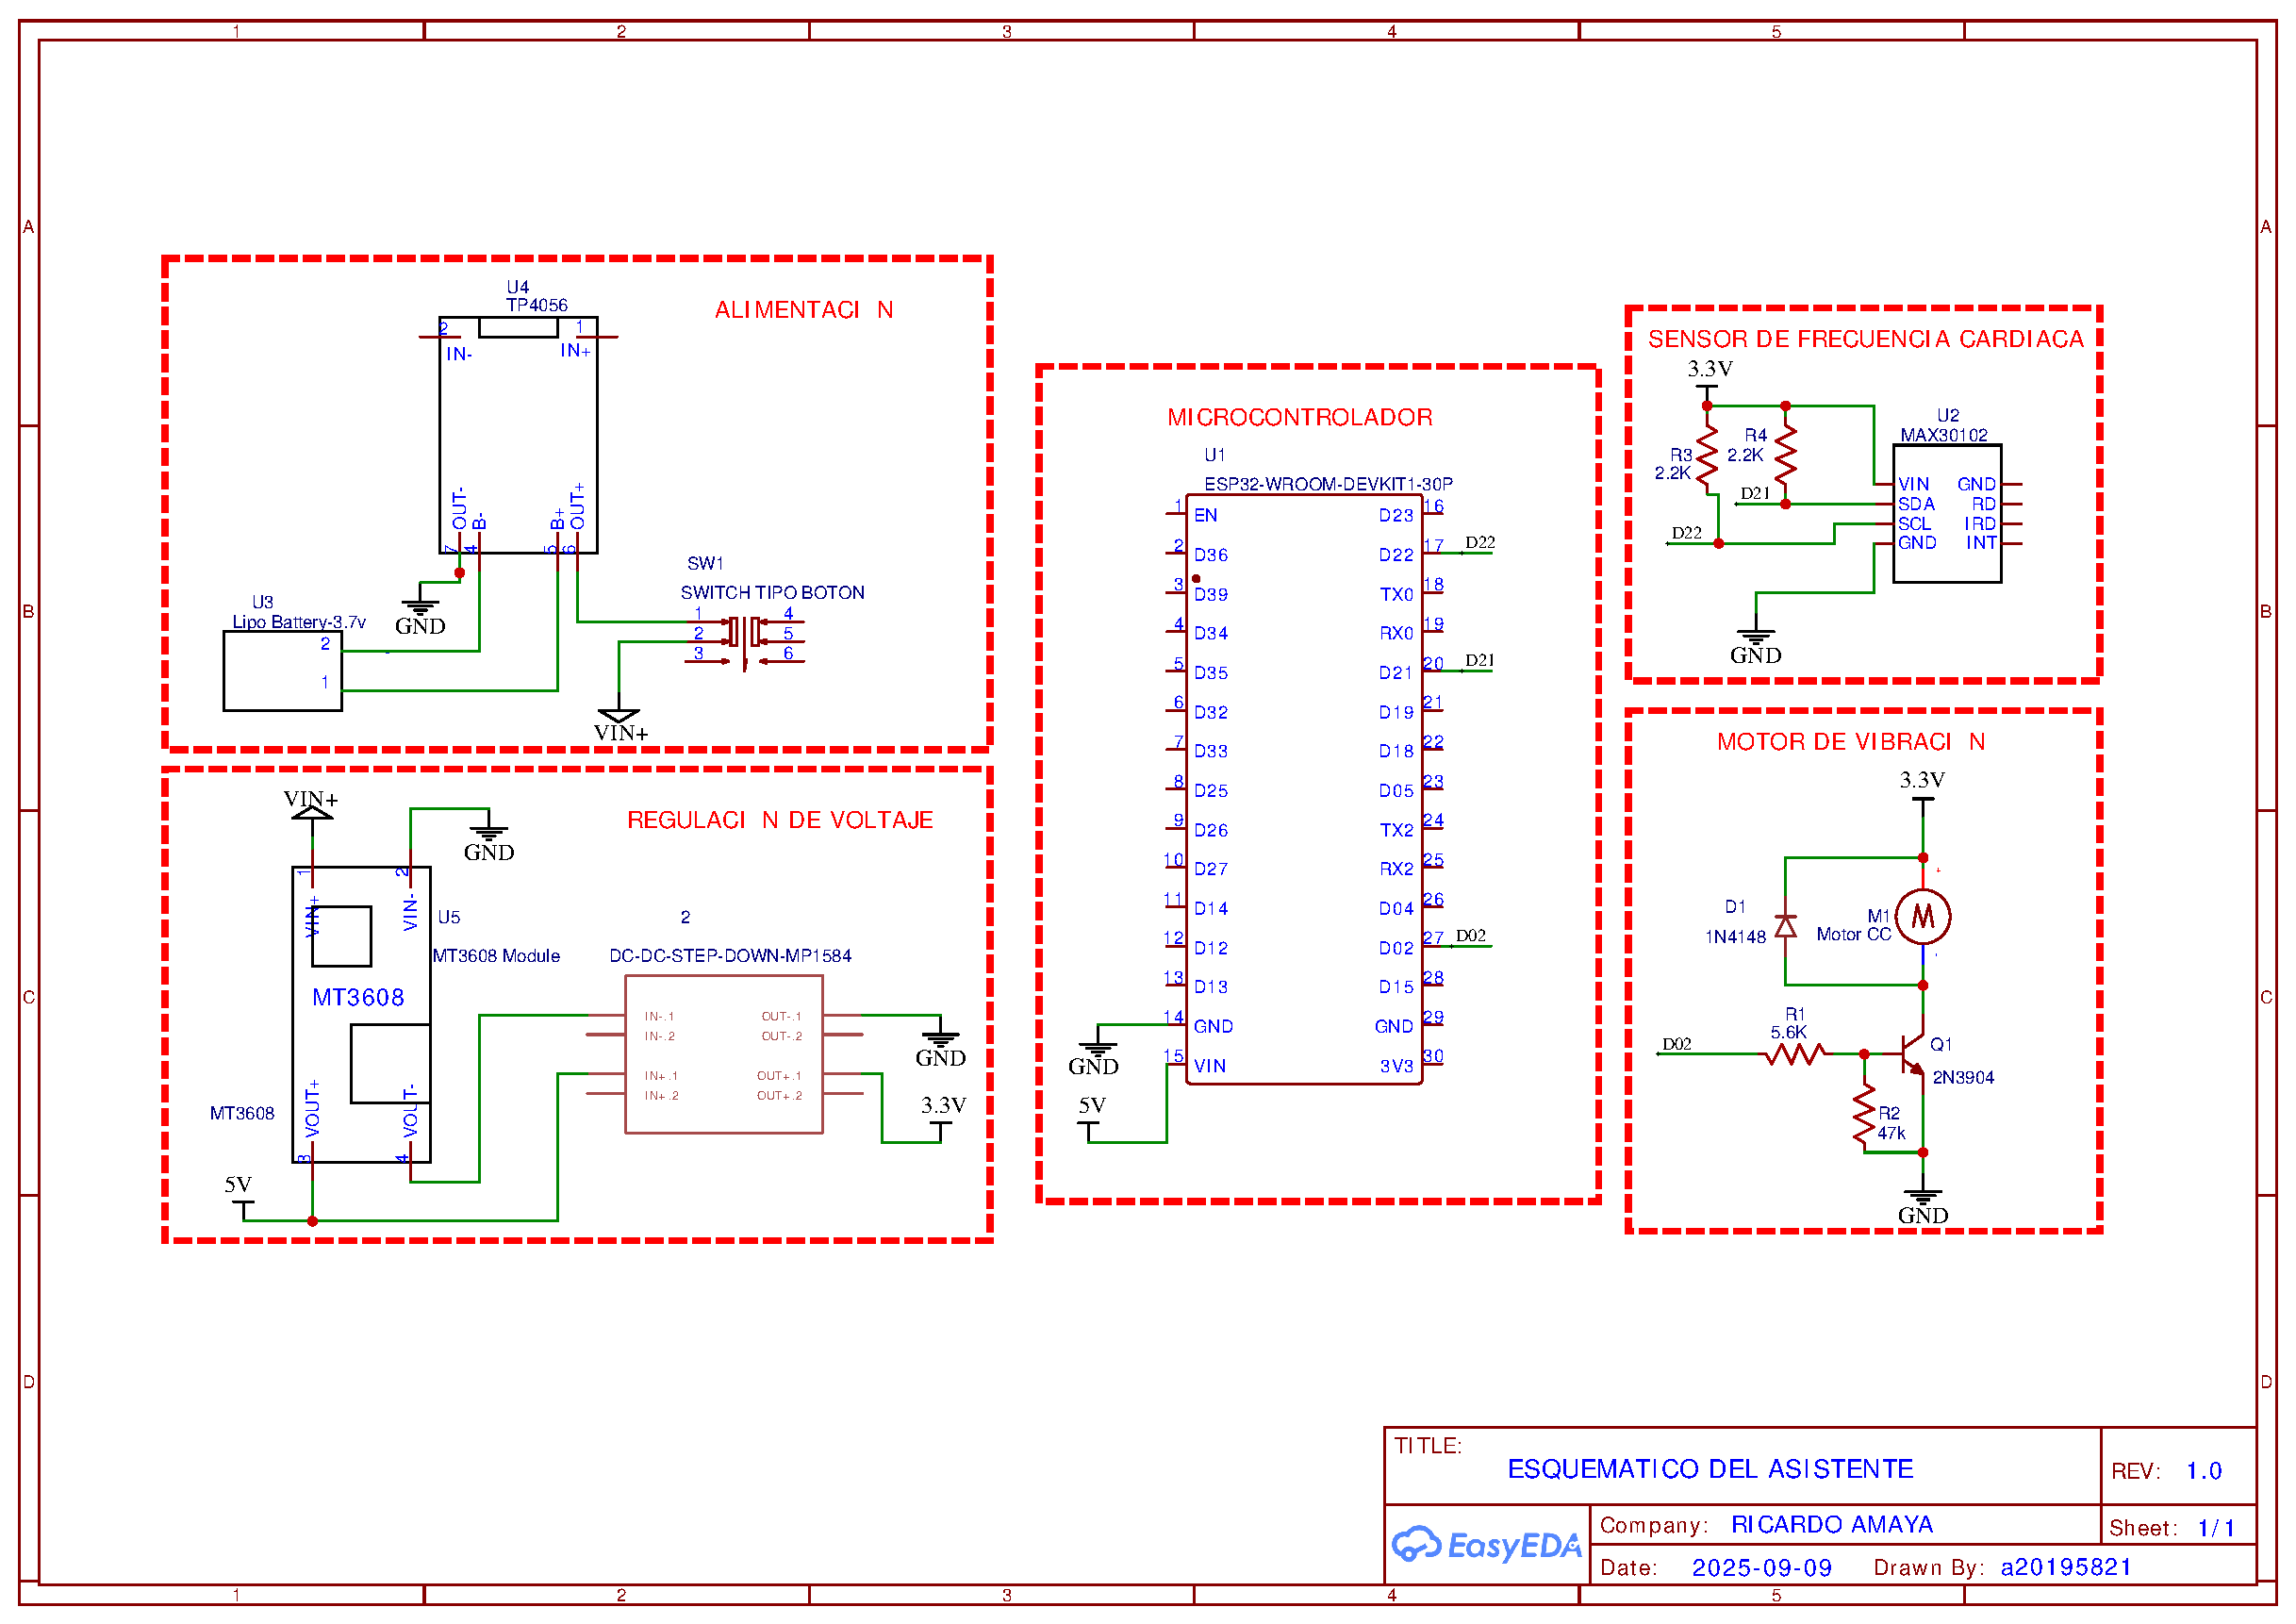
\includegraphics[angle=90, width=0.95\textwidth]{CHPTRS/CH04_DISEÑO/imagenes/Esquematico.pdf}
    \caption{Esquemático del asistente}
    \label{fig:4.esquematico}
\end{figure}






\subsection{Diseño de PCB}
En las Figuras~\ref{fig:4.PCBS} y  se aprecia el diseño realizado de una PCB de potencia para el asistente. En este se ubican ambos reguladores, el módulo de carga el circuito de protección del motor, así como los conectores para la batería, motor y sensor.

\begin{figure}[H]
    \centering
    % Primera imagen
    \begin{subfigure}{0.4\textwidth}
         \centering
            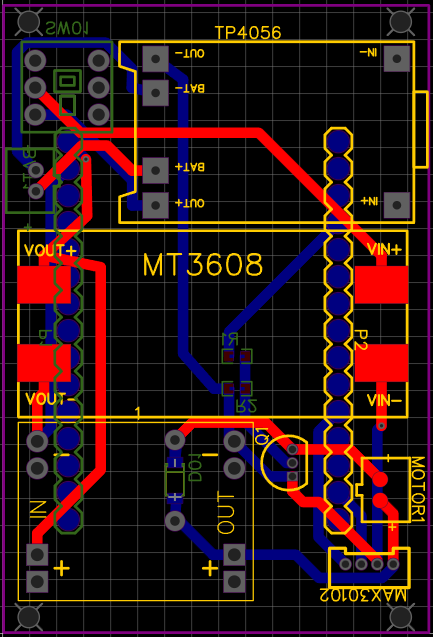
\includegraphics[width=\textwidth]{CHPTRS/CH04_DISEÑO/imagenes/pcb.png}
            \caption{PCB diseñada}
            \label{fig:4.pcb}
            \captionsetup{justification=centering,margin=1cm}
    \end{subfigure}
    \hfill
    % Segunda imagen
    \begin{subfigure}{0.4\textwidth}
       
        \centering
        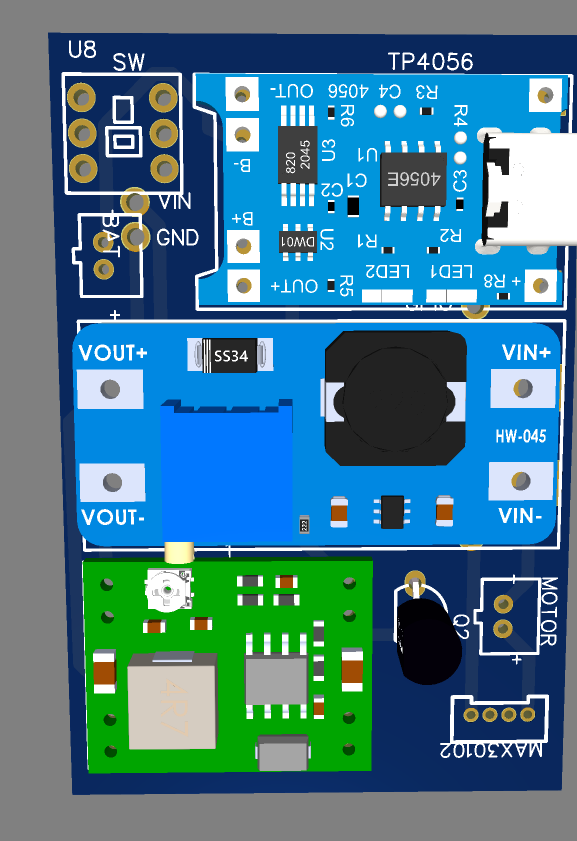
\includegraphics[width=\linewidth]{CHPTRS/CH04_DISEÑO/imagenes/pcb 3d.png}
        \caption{vista 3D de la PCB}
        \label{fig:4.pcb3d}
        
    \end{subfigure}

    \caption{PCB de potencia diseñada}
    \label{fig:4.PCBS}
     \end{figure}   
\section{Diseño mecánico}

\subsection{Selección del material de correa}
Para poder seleccionar el material de la correa, se debe tener en cuenta el peso de los componentes, cuyos pesos se encuentran en la Tabla~\ref{tab:4.pESOS} y la aceleración de una persona al realizar movimientos. Teniendo en cuenta que el asistente será utilizado en ambientes de estudio tradicionales, se tiene que considerar movimientos controlados. Según \textcite{4.aceleración}, un movimiento controlado se define en un rango entre 4.36 y 5.38 m/s² en el brazo. En ese trabajo se consideró un valor aproximado de 5.38 m/s² y un factor de seguridad de 2.

    \begin{table}[H]
    \centering
    \caption{Pesos de los componentes}
    \label{tab:4.pESOS}
    \begin{tabular}{|c|c|} 
    \hline
    Componente       & Peso    \\ 
    \hline
    módulo ESP32     & 9 g     \\ 
    \hline
    MAX30102         & 8 g     \\ 
    \hline
    Módulo de carga  & 2 g     \\ 
    \hline
    Regulador MT3608 & 5 g     \\ 
    \hline
    Regulador MP1584 & 3 g     \\ 
    \hline
    Batería          & 18.1 g  \\ 
    \hhline{|==|}
    Total            & 45.1 g  \\
    \hline
    \end{tabular}
    \end{table}
Asimismo, a través de la selección de componentes se ha determinado unas dimensiones máximas de 65x45x30 mm. Considerando que la carcasa tenga un peso aproximado de 30 gramos, se tiene una masa de $0,0751 \,kg$ en total y a través de la Ecuación~\ref{ec:4.Finerciasl} se puede hallar la fuerza inercial producto del movimiento que realice el usuario.
\begin{align}
\label{ec:4.Finerciasl}
F=m\,a\,\,\,[\si{\newton}]
\end{align}
De esta manera, se tiene una fuerza $F_1 =0.404\,N$. Ahora, se debe tener en cuenta la fuerza de fricción para evitar el deslizamiento del asistente, la cual debe ser mayor que la fuerza calculada previamente. La fuerza de fricción se obtiene mediante la Ecuación~\ref{ec:4.Ffircvcion}, donde  se multiplica la presión en el brazo $p\,\,\,[\si{\pascal}]$, el coeficiente de fricción $\mu$ y el área de contacto entre correa y la piel $A_c\,\,\,[\si{\milli\meter}^2]$.
\begin{align}
\label{ec:4.Ffircvcion}
F_{fric}=p\,\mu \,A_c \,\,\,[\si{\newton}]
\end{align}
Al tener en cuenta la relación $F_{fric}>F_{iner}$ y despejar la presión $p\,\,\,[\si{\pascal}]$ se obtiene la Ecuación~\ref{ec:4.presionl}, donde la fricción $\mu$ depende del material de la correa y se toma un área de contacto $A_c =  \SI{6000}{\milli\meter^2} $ con un ancho de $\SI{20}{\milli\meter}$ con una longitud efectiva de $\SI{300}{\milli\meter}$ perteneciente a un universitario aproximadamente, ya que esta longitud efectiva varia por persona.
\begin{align}
\label{ec:4.presionl}
p>\frac{F_{iner}}{\mu\,A_c} \quad\Rightarrow\quad \mu>\frac{F_{iner}}{p\,A_c}
\end{align}

Según \textcite{4.presion}, para que una persona no sienta incomodidad o restricción del flujo sanguíneo por la presión, se tiene un rango de 20 a 30 mmHg. En este caso se ha seleccionado a 25 mmHg como presión máxima, la cual equivale a  $3333.06 \approx \SI{3333}{\pascal}  $. Asimismo, despejando el coeficiente de fricción $\mu$ y reemplazado con los valores $F_{iner} = F_1=0.404\,N$, $A_c =  \SI{6000}{\milli\meter^2}$ y $p =  \SI{3333}{\pascal}$, se puede determinar el coeficiente de fricción mínimo que se tiene para evitar deslizamiento y asegurar confort (ver Ecuación~\ref{ec:4.mumin}).
\begin{align}
\label{ec:4.mumin}
\mu_{min}>0.0202\,FS
\end{align}

Al multiplicar por el factor de seguridad, se obtiene $\mu_{min} =0,0404$, lo cual al ser muy pequeño, nos permite una gran posibilidad de materiales de correa. En un estudio realizado por \textcite{4.correas}, se indica que el coeficiente de fricción en la piel es de un promedio de
$0,46\,\pm\,0,154$, siendo la silicona el material con un mayor coeficiente (0,6) y el nylon es aquel que cuenta con menor coeficiente de fricción (0,37). Sin embargo, en el presente trabajo se optó por utilizar nylon debido a su disponibilidad y ha sido utilizado previamente en dispositivos deportivos, lo cual asegura confort para el usuario.


\subsection{Selección del material de carcasa}
En el caso de la carcasa, se tiene como opciones de material PETG y ABS, cuyas características principales se encuentran en la Tabla~\ref{tab:4.Caracteristicas materiales} . Ambos materiales son buenas opciones porque permiten tener ligereza, confort y rigidez. El material ABS permitiría un acabado más profesional ya que es comúnmente utilizado en diversos dispositivos. Sin embargo, tiene un mayor costo y una mayor dificultad de impresión debido a la expulsión de gases. Por ello, en este trabajo se optó por desarrollar la carcasa con el material PETG. 

\begin{table}[H]
\centering
\caption{Características de los materiales PETG y ABS}
\label{tab:4.Caracteristicas materiales}
\begin{tblr}{
  cells = {c},
  hlines,
  vlines,
}
Características            & PETG      & ABS       \\
Densidad                   & 1.23g/cm3 & 1.01g/cm3 \\
Módulo de elasticidad      & 2.0GPa    & 2.0GPa    \\
Resistencia a tracción     & 50MPa     & 40MPa     \\
Facilidad de impresión     & Alta      & Baja      \\
Temperatura de deformación & 80°C      & 105°C     
\end{tblr}
\end{table}

\subsection{Modelado de la carcasa}

En la Figura~\ref{fig:4.modelado} se puede observar la figura del modelado 3D del asistente, este tiene unas dimensiones finales 65 x 45 x 29.5 milímetros. A continuación se detallará las uniones con los diversos componentes. Asimismo, los planos mecánicos se encuentran en Anexos~\ref{an:Annex_E_Planos_Mecánicos}.

%\begin{figure}[H]
    %\centering
    %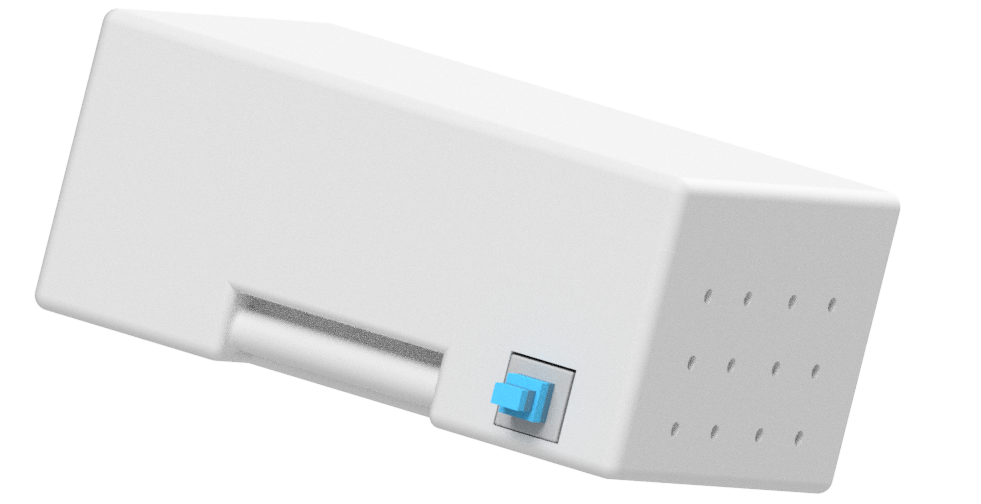
\includegraphics[width=0.8\textwidth]{CHPTRS/CH04_DISEÑO/imagenes/imag_3d/ensamble.png}
    %\caption{Modelado 3D del asistente}
    %\label{fig:4.modelado}
    %\captionsetup{justification=centering,margin=1cm}
   % \end{figure}
\subsubsection{Parte superior de la Carcasa}
En la siguiente Figura~\ref{fig:4.modeladoSUPERIOR} se puede apreciar la parte superior de la carcasa. Esta cuenta con un orificio donde estará colocado la batería por inserción, de manera que también se pueda retirar de manera sencilla en caso de mantenimiento. Sin embargo, cuenta con una barra de material que sirve de inserción con la parte inferior de la carcasa por motivos solo de prototipado, ya que la unión entre estas debe ser mediante pegamento.


%\begin{figure}[H]
    %\centering
    %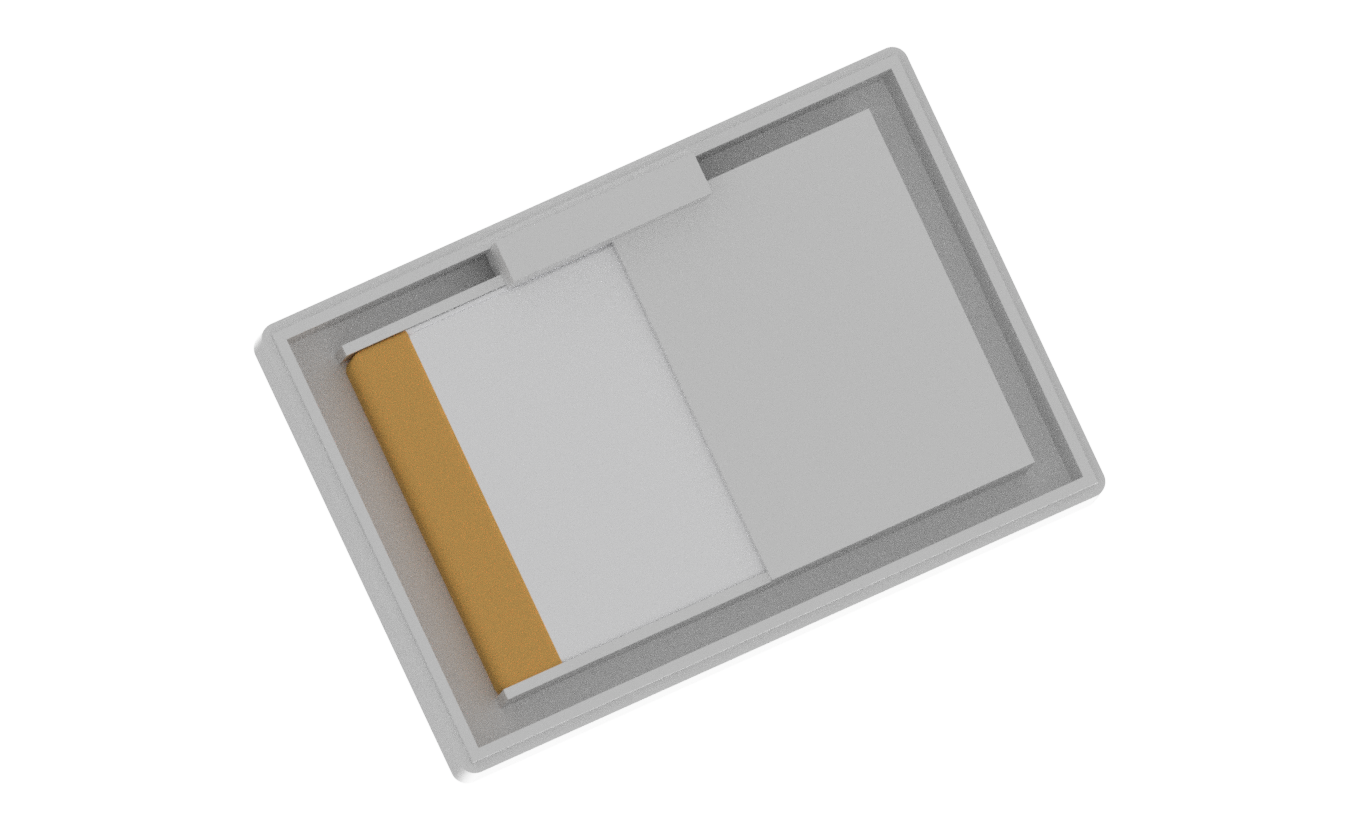
\includegraphics[width=0.9\textwidth]{CHPTRS/CH04_DISEÑO/imagenes/imag_3d/superior.png}
   % \caption{Modelado parte superior de la carcasa}
  %  \label{fig:4.modeladoSUPERIOR}
   % \captionsetup{justification=centering,margin=1cm}
   % \end{figure}

\begin{figure}[H]
    \centering
    % ---- Figura 1 ----
    \begin{minipage}[t]{0.48\textwidth}
        \centering
        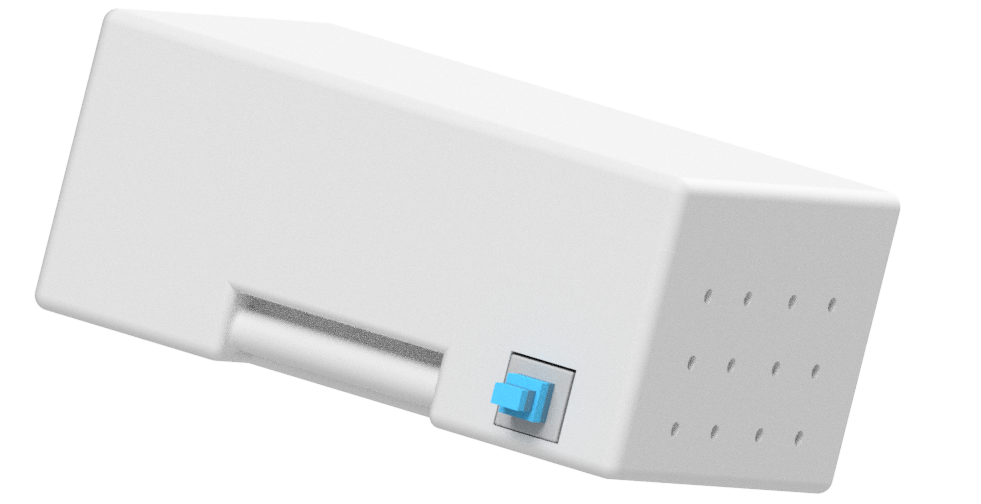
\includegraphics[width=\textwidth]{CHPTRS/CH04_DISEÑO/imagenes/imag_3d/ensamble.png}
        \captionof{figure}{Modelado 3D del asistente}
        \label{fig:4.modelado}
    \end{minipage}
    \hfill
    % ---- Figura 2 ----
    \begin{minipage}[t]{0.48\textwidth}
        \centering
        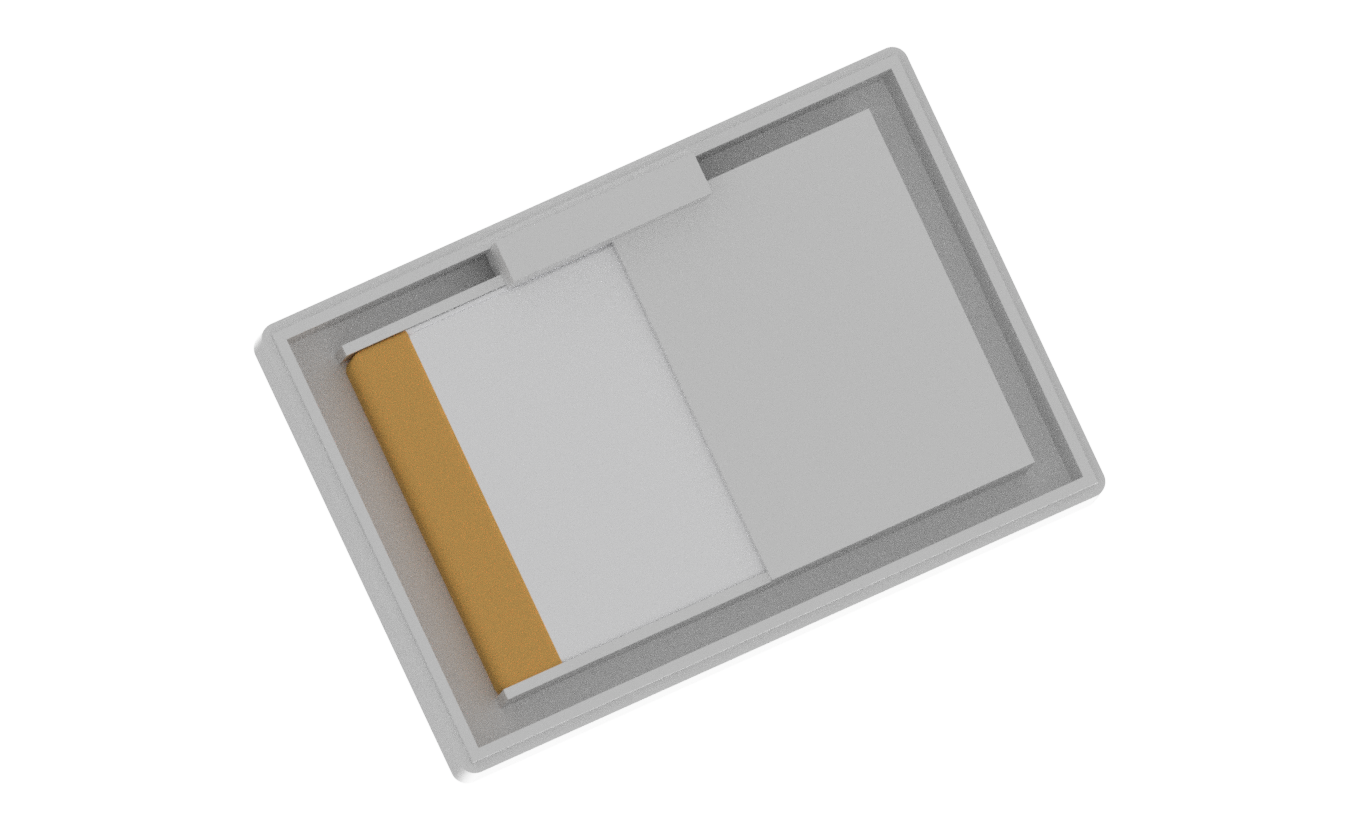
\includegraphics[width=\textwidth]{CHPTRS/CH04_DISEÑO/imagenes/imag_3d/superior.png}
        \captionof{figure}{Modelado parte superior de la carcasa}
        \label{fig:4.modeladoSUPERIOR}
    \end{minipage}

    \captionsetup{justification=centering,margin=1cm}
\end{figure}


\subsubsection{Parte inferior de la Carcasa}
La Figura~\ref{fig:4.modeladoBase} muestra la parte inferior de la carcasa. En ella se puede observar que tiene orificios circulares en las caras laterales para ventilación y cuenta con todos los bordes bordeados para protección, ya que la parte baja de esta base estará en contacto directo con la piel del usuario.

\begin{figure}[H]
    \centering
    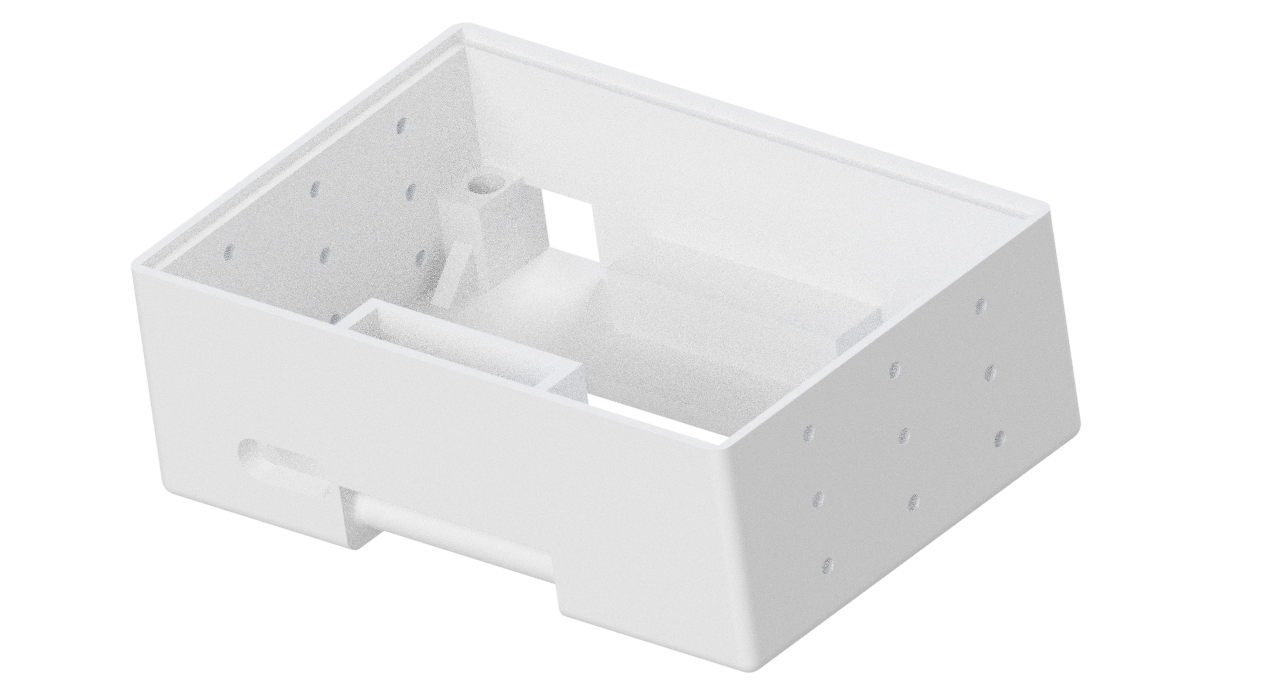
\includegraphics[width=0.7\textwidth]{CHPTRS/CH04_DISEÑO/imagenes/imag_3d/Base.png}
    \caption{Modelado parte Inferior de la carcasa}
    \label{fig:4.modeladoBase}
    \captionsetup{justification=centering,margin=1cm}
    \end{figure}


Asimismo, tiene espacios donde se colocará el sensor MAX30102 y el motor de vibración que serán colocados por encaje a presión. Asimismo, tiene una caja donde será colocada la barra de inserción de la parte superior, como se mencionó previamente, este es solo para prototipado, ya que ambas partes irán pegadas. 
\begin{figure}[H]
    \centering
    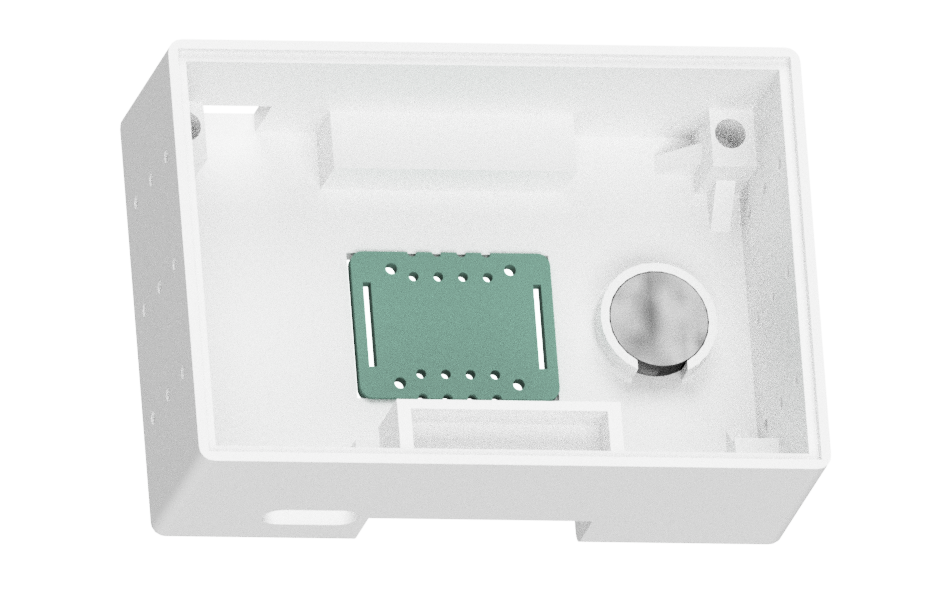
\includegraphics[width=0.8\textwidth]{CHPTRS/CH04_DISEÑO/imagenes/imag_3d/Base_MOTOR_sENSOR.png}
    \caption{Encajes de presión para el sensor MAX3012 y el motor de vibración}
    \label{fig:4.modeladoBase}
    \captionsetup{justification=centering,margin=1cm}
    \end{figure}

Además, cuenta con un espacio para que el usuario pueda insertar el conector de tipo C para poder recargar el asistente a través del módulo TP4056 y un agujero donde está colocado el botón de encendido y apagado por presión (ver Figuras~\ref{fig:4.BaseUSB} y~\ref{fig:4.BaseBOTON} respectivamente).
\begin{figure}[H]
    \centering
    % Primera imagen
    \begin{subfigure}{0.4\textwidth}
        \centering
        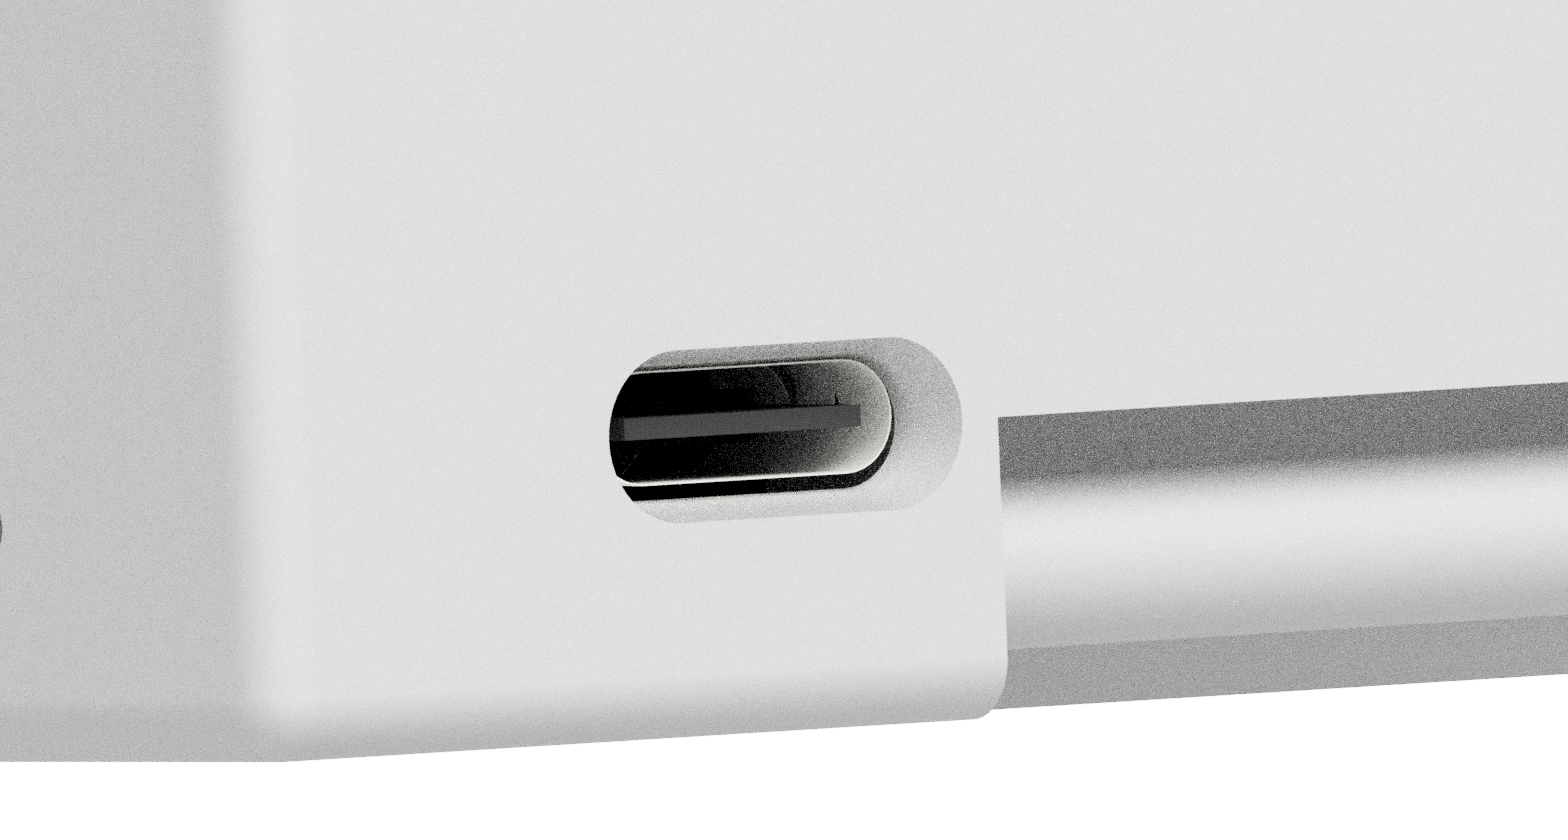
\includegraphics[width=\linewidth]{CHPTRS/CH04_DISEÑO/imagenes/imag_3d/ensamble_usb.png}
        \caption{Espacio para la carga del asistente}
        \label{fig:4.BaseUSB}
        
    \end{subfigure}
    \hfill
    % Segunda imagen
    \begin{subfigure}{0.32\textwidth}
       

        \centering
        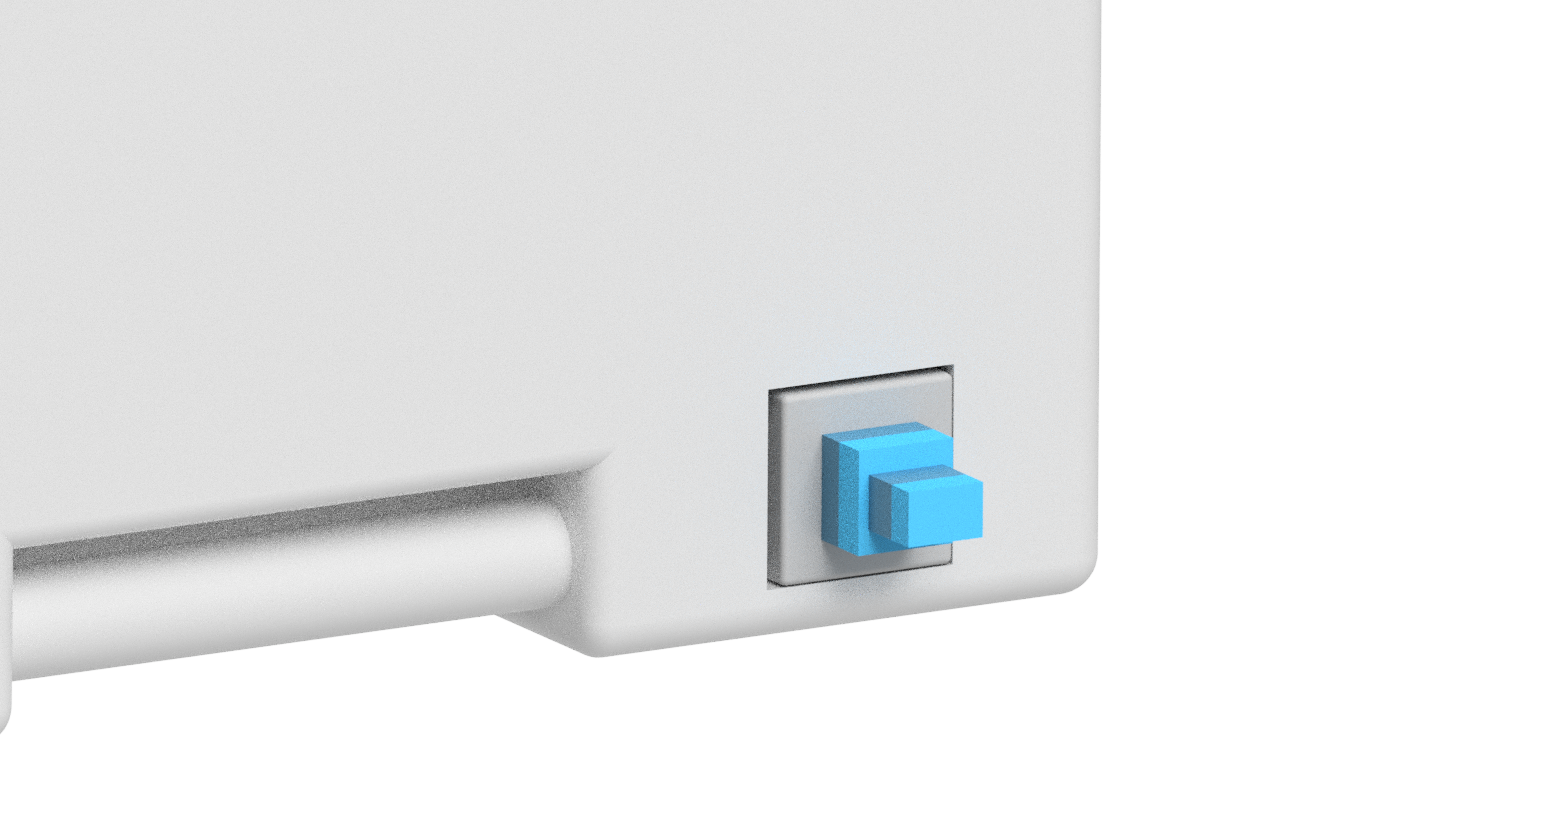
\includegraphics[width=\linewidth]{CHPTRS/CH04_DISEÑO/imagenes/imag_3d/ensamble_boton.png}
        \caption{Espacio para el botón del asistente}
        \label{fig:4.BaseBOTON}
        
    \end{subfigure}
    \caption{Espacios para el cargador y el botón}

\end{figure}

\subsection{Sujeción de correa}
En la carcasa se tienen barras circulares en ambos lados como se puede apreciar en la Figura~\ref{fig:4.cilindros}. Estas serán las encargadas de sujetar la correa y para determinar el diámetro del cilindro se consideró una longitud $L_1 =23\,mm$, fuerza de tensión $F_1=40\,\si{\newton}$. Esta se tuvo como aproximación en base a un estudio realizado por \textcite{4.diametro} , donde determinaron que se utilizaban tensiones de entre 20 y 60 \si{\newton} en las correas para un tratamiento de escoliosis; sin embargo, en este caso no se busca realizar un tratamiento de ajuste y se decidió optar por el valor promedio de este estudio.\\

A través de la Ecuación~\ref{ec:mmax} para sistemas empotrados  se determino el momento flector máximo $M_{max}=115 \,\si{\newton}.mm $ que soporta la barra circular empotrada en ambos lados. Posteriormente se utilizó la Ecuación~\ref{ec:diametro}, la cual fue despejado en base a las propiedades de una barra circular para poder determinar el diámetro mínimo que necesita tener el cilindro.

\begin{align}
\label{ec:mmax}
M_{max}= \frac{F_1\,L_1}{8}\,\,\,[\si{\newton}.mm]
\end{align}

\begin{align}
\label{ec:diametro}
\sigma = \frac{M_{\text{max}}\,c}{I} 
\quad\Rightarrow\quad 
d_{min}^3 > \frac{32\,M_{\text{max}}}{\pi\,\sigma}
\end{align}

De esta manera, considerando que el material tiene una resistencia de $\sigma = 50\,M\si{\pascal}$ (ver Tabla~\ref{tab:4.Caracteristicas materiales}) y reemplazando el valor de $M_{max}=115 \,\si{\newton}.mm $ se obtiene un diámetro mínimo $d_{min}= 2.86\,\si{\milli\meter} $. En el caso de la carcasa, se ha seleccionado un diámetro de 4 mm con un factor de seguridad de 1,39 aproximadamente.

\begin{figure}[H]
    \centering
    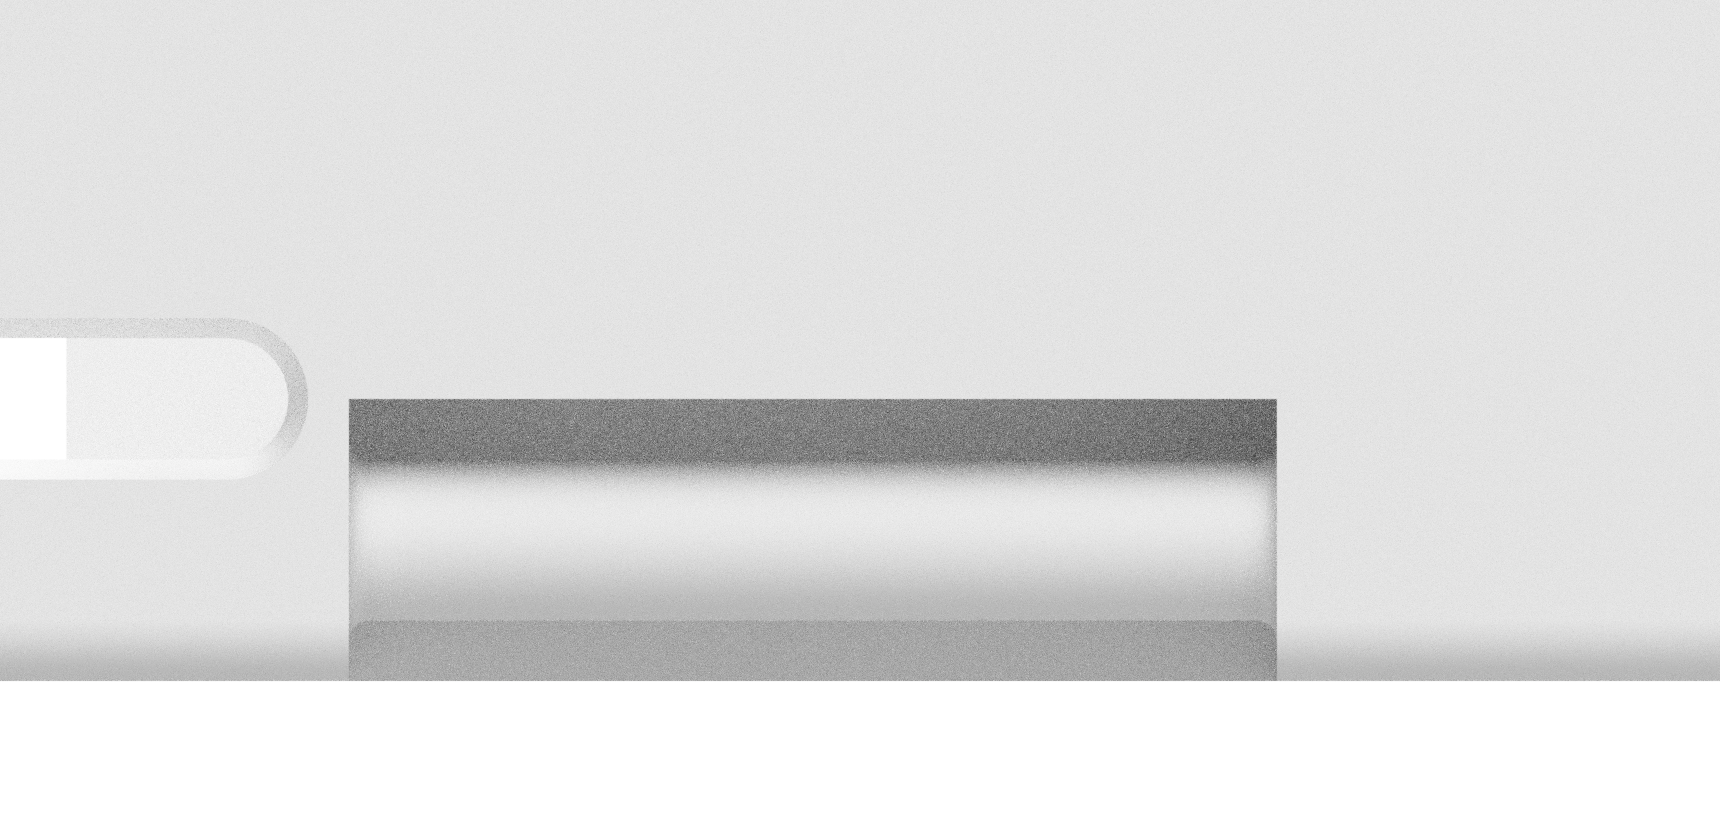
\includegraphics[width=0.8\textwidth]{CHPTRS/CH04_DISEÑO/imagenes/imag_3d/Base_cilindro.png}
    \caption{Barra de sujeción}
    \label{fig:4.cilindros}
    \captionsetup{justification=centering,margin=1cm}
    \end{figure}
\subsection{Sujeción de tarjeta electrónica}
Para la sujeción de la tarjeta electrónica, se han colocado 4 agujeros roscados en los extremos de la carcasa como el que se encuentra en la Figura\ref{fig:4.agujero}. Estas cuentan con un agujero donde se colocan insertos roscados para impresión 3D M2x3 junto con los tornillos M2x6 (ver Figura~\ref{fig:4.tornillo}, considerando que solo soportaran el peso de unos 50 gramos aproximadamente. No hay ningún inconveniente con utilizar estos tornillos.

\begin{figure}[H]
    \centering
    % Primera imagen
    \begin{subfigure}{0.5\textwidth}
        \centering
        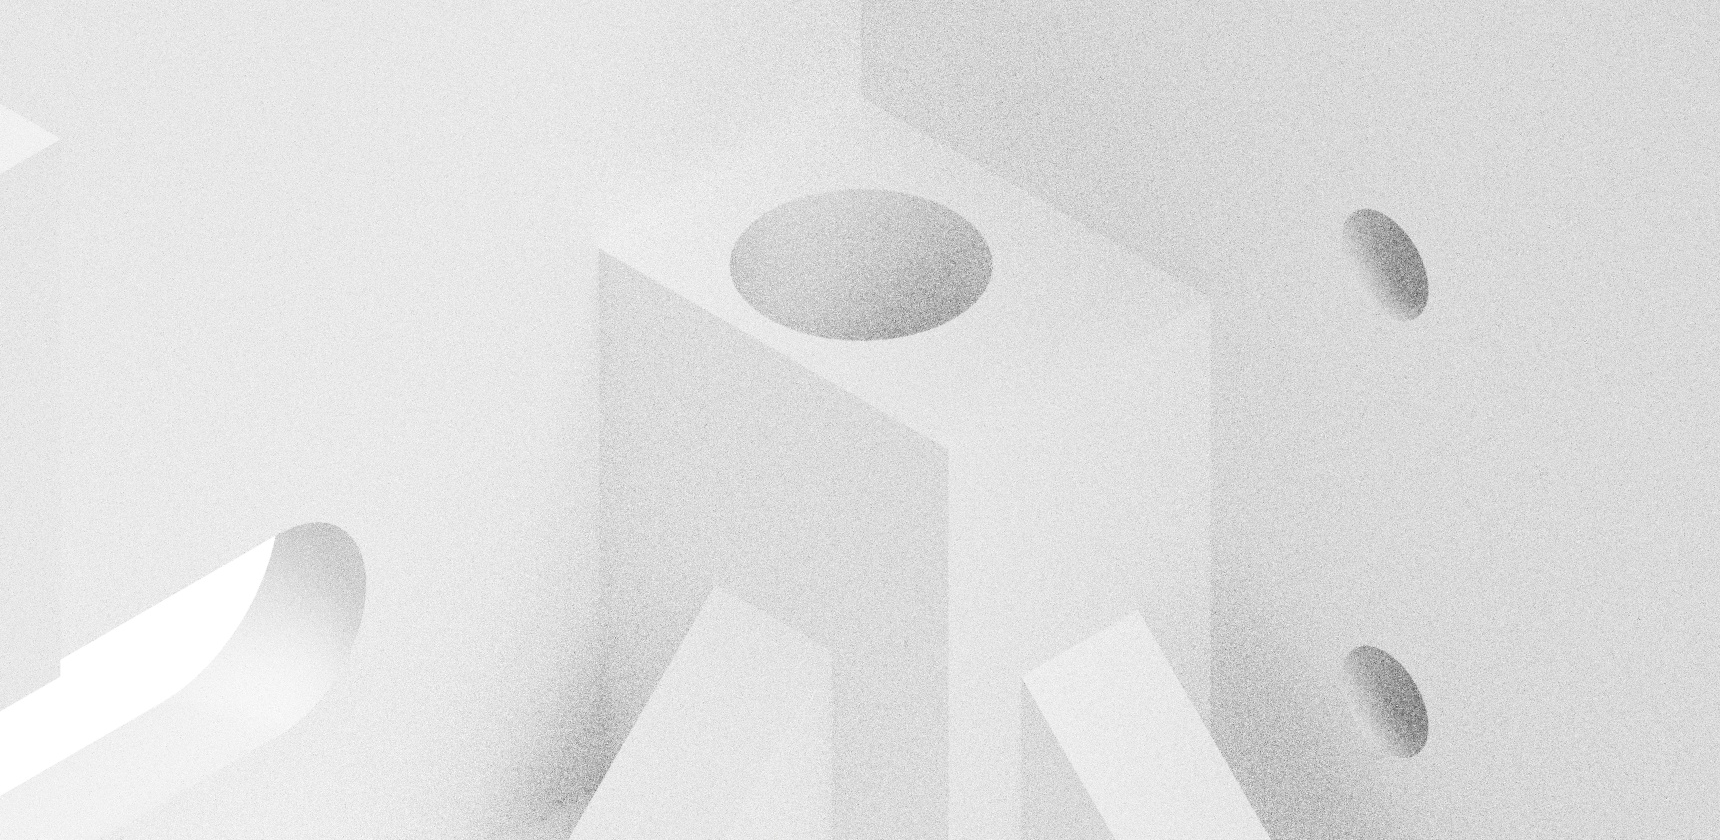
\includegraphics[width=\linewidth]{CHPTRS/CH04_DISEÑO/imagenes/imag_3d/Base_agujero.png}
        \caption{Agujero de sujeción}
        \label{fig:4.agujero}
        
    \end{subfigure}
    \hfill
    % Segunda imagen
    \begin{subfigure}{0.32\textwidth}
       

        \centering
        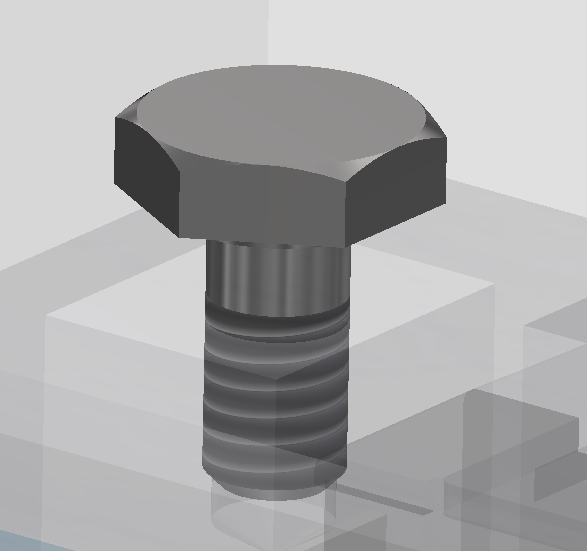
\includegraphics[width=0.8\linewidth]{CHPTRS/CH04_DISEÑO/imagenes/imag_3d/tornillo.png}
        \caption{Tornillo de sujeción}
        \label{fig:4.tornillo}
        
    \end{subfigure}
    \caption{Sujeción de tarjeta electrónica}

\end{figure}

%%%%%%%%%%%%%%%%%SOFTWARE%%%%%%%%%%%%%%%%%%%
\section{Diseño del software}
\subsection{Sistema}
Para el desarrollo de la programación, considerando que se utiliza un microcontrolador ESP32, se ha utilizado \textit{PlatformIO}, el cual es una herramienta que permite escribir aplicaciones para productos embebidos. Asimismo, se utilizó la librería \verb|ESP32 BLE Arduino @ ^1.0.1| para el manejo del ESP32, la librería \verb|SparkFun MAX3010x Pulse and Proximity Sensor Library @ ^1.1.2| para el manejo del sensor MAX30102 y la librería \verb|kosme/arduinoFFT@^2.0.4| para el procesamiento de la señal. Asimismo el código de programación utilizado se encuentra en Anexos.

\subsubsection{Conexión BLE}
La implementación de la conexión \textit{Bluetooth Low Energy (BLE)} se realizó mediante las librerías del mismo ESP32 (BLEDevice, BlEServer y BLEUtils). Una de las funciones principales es \textit{InitBLE()} donde se define el nombre del dispositivo, se crea un servidor BLE con un servicio, el cual cuenta con permisos de lectura y transmisión. Otra de las funciones principales es \textit{startAdvertising()} que permite que cualquier dispositivo móvil cercano pueda detectarlo. En esta función se envía el nombre del dispositivo y el identificador del servicio para facilitar su identificación. Asimismo, para la facilidad de su identificación, se le asignó el nombre de 'Asistente Cognitivo'.

\subsubsection{Procesamiento de la señal}
En este caso, el sistema inicia identificando la presencia o ausencia de contacto entre el sensor y la piel, mediante los valores extraídos del LED infrarrojo del MAX3012. Esta señal infrarroja se suaviza mediante un promedio móvil simple de 10 muestras para reducir el ruido y cuando supera un umbral mínimo, habilita el procesamiento del pulso.\\

Una vez establecido el contacto, la señal suavizada es sometida a un umbral calculado a partir del rango dinámico de la señal a través de la diferencia entre el máximo y mínimo de la señal. Este umbral se actualiza continuamente para compensar cambios en la señal producidas por diferentes usuarios. Posteriormente, se produce la detección de pulsos, cuando la señal supera el umbral y posteriormente desciende, se considera que ha ocurrido un latido.\\
Finalmente, con los latidos detectados se calcula el tiempo entre pulsos sucesivos (RR) y, a partir de este, la frecuencia cardíaca instantánea (BPM). Adicionalmente, se descartan valores fisiológicamente irregulares. Por ejemplo, no se toma en cuenta frecuencias mayores a 140 BPM. El diagrama de flujo para el procesamiento se encuentra en la Figura~\ref{fig:cod.sensor}.

\begin{figure}[H]
\centering
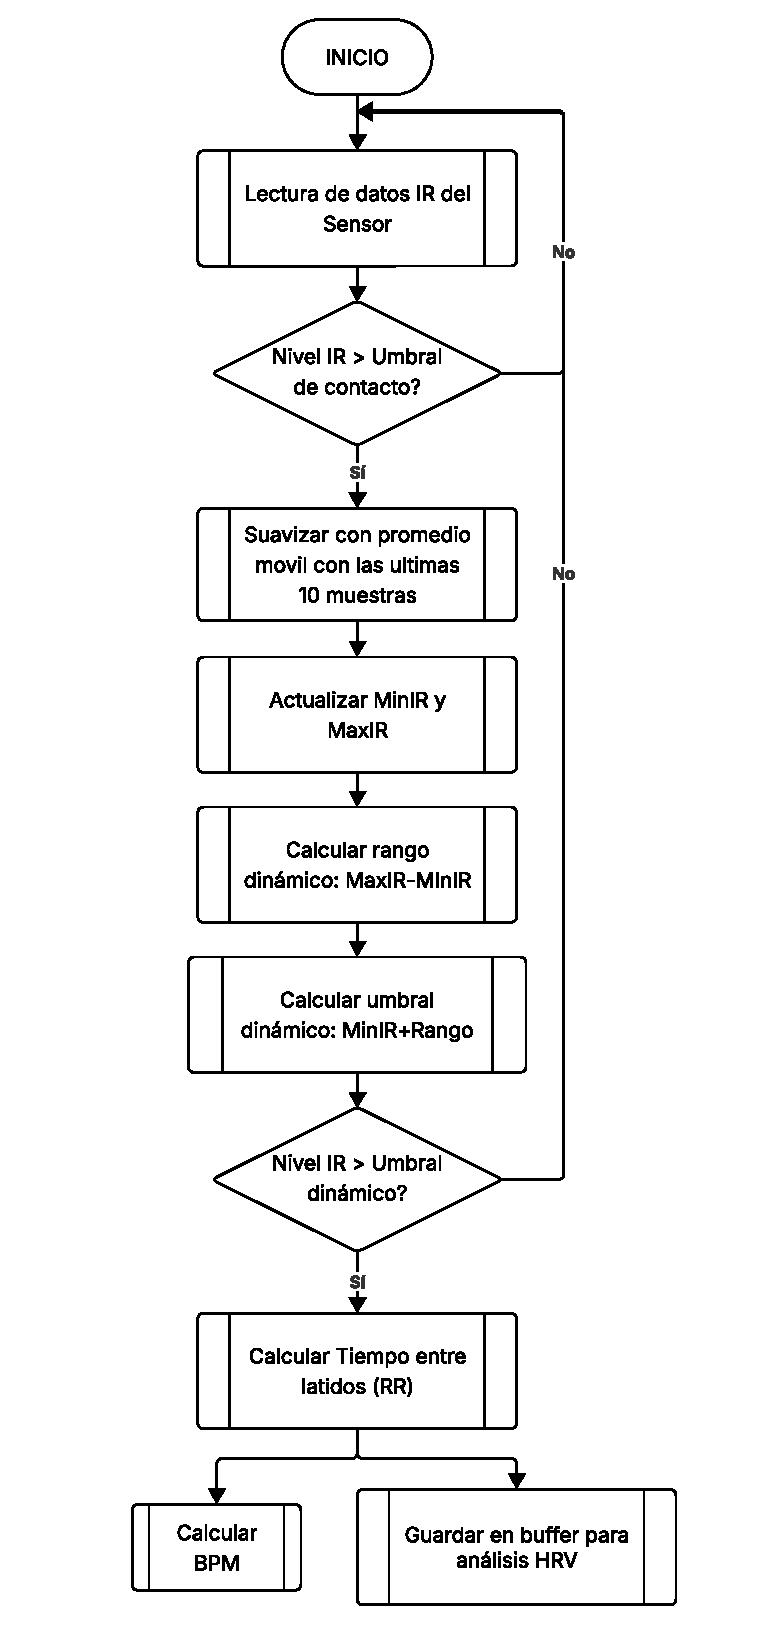
\includegraphics[width=0.5\textwidth]{CHPTRS/CH04_DISEÑO/imagenes/imag_cod/Diagrama procesamiento.pdf}
\caption{Diagrama de flujo del procesamiento de la señal}
\label{fig:cod.sensor}
\captionsetup{justification=centering,margin=1cm}
%\caption*{\textit{Elaboración propia}}
\end{figure}
\cleardoublepage





\subsubsection{Clasificación de Estados de concentración}

Para poder realizar el modelo de clasificación, se debe tener en consideración lo explicado en la Sección~\ref{sec:frecuenciaC}. Es decir, que una menor relación \ac{LF}/\ac{HF} es indicativo de una mayor atención sostenida, caso contrario es distracción, ya que esta será la base del clasificador realizado.\\

En este caso, los tiempos entre pulsos sucesivos (RR) detectados en el procesamiento de la señal son acumulados y, considerando que estos  tiempos son irregulares, se realiza una interpolación lineal. Posteriormente, se utiliza Transformada de Fourier, ya que permite transformar la serie temporal de intervalos RR en su representación espectral. Este espectro permite calculas las bandas de baja frecuencia \ac{LF}, las de ata frecuencia \ac{HF} y, en consecuencia, la relación entre estas.\\

Sin embargo, debido a que esta relación varía notablemente entre individuos, el sistema tiene un tiempo de calibración inicial, donde a través de los valores LF/HF, se construye un baseline personalizado para el usuario, la cual se basa en el promedio de los valores validos durante el periodo de calibración.\\

Finalmente, se introduce un indice basado entre el valor actual de LF/HF y el baseline del usuario. Este indice permite determinar el estado de concentración del usuario, donde un valor significativamente menor al baseline  es catalogado como Alta concentración, cercanos como concentración moderada y valores muy superiores se asocian a distracción o falta de atención. En la siguiente Figura~\ref{fig:cod.clasficacion} se aprecia el diagrama de flujo para la clasificación

\begin{figure}[H]
\centering
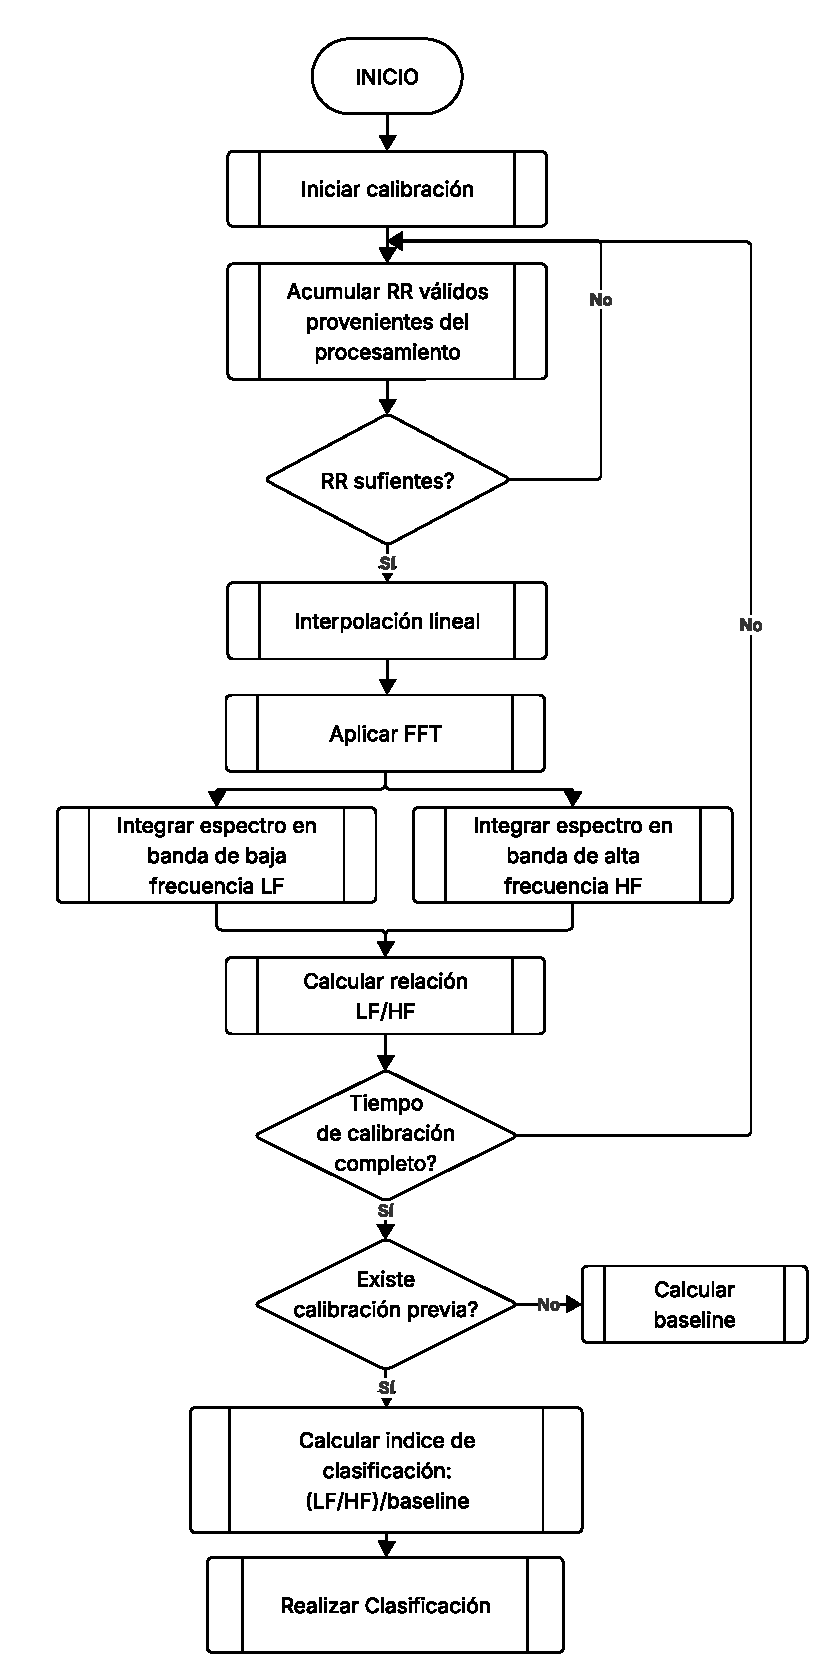
\includegraphics[width=0.6\textwidth]{CHPTRS/CH04_DISEÑO/imagenes/imag_cod/Diagrama clasificacion.pdf}
\caption{Diagrama de flujo de la clasificación}
\label{fig:cod.clasficacion}
\captionsetup{justification=centering,margin=1cm}
%\caption*{\textit{Elaboración propia}}
\end{figure}





\subsection{Interfaz}
El desarrollo del prototipado de  la interfaz se realizó mediante \textit{Flutter} en \textit{Android Studio}. Este esta pensando para que sea intuitivo para el usuario, de manera de que no tenga problemas al momento de establecer conexión y empezar su sesión de estudio. El código de esta interfaz se encuentra en Anexos.
\subsubsection{Conexión}
Esta sección corresponde a la pantalla inicial del aplicativo (ver Figura~\ref{fig:interfaz.conexion}). En esta, el usuario puede establecer conexión mediante BLE con el asistente de manera automática, ya que siempre se busca al dispositivo con dicho nombre. Asimismo, se tiene un botón que permite acceder al menú principal sin la necesidad de establecer conexión para que el usuario pueda acceder a su historial. 

\subsubsection{Menú principal}
En esta interfaz que se puede apreciar en la Figura~\ref{fig:interfaz.menu}, el usuario accede una vez establecida la conexión BLE con el asistente de concentración. Además tiene la posibilidad de acceder a las demás pestañas, las cuales son 'Iniciar Sesión de estudio', 'Historial' y 'Configuración'.

\begin{figure}[H]
    \centering
    % Primera imagen
    \begin{subfigure}{0.4\textwidth}
        \centering
        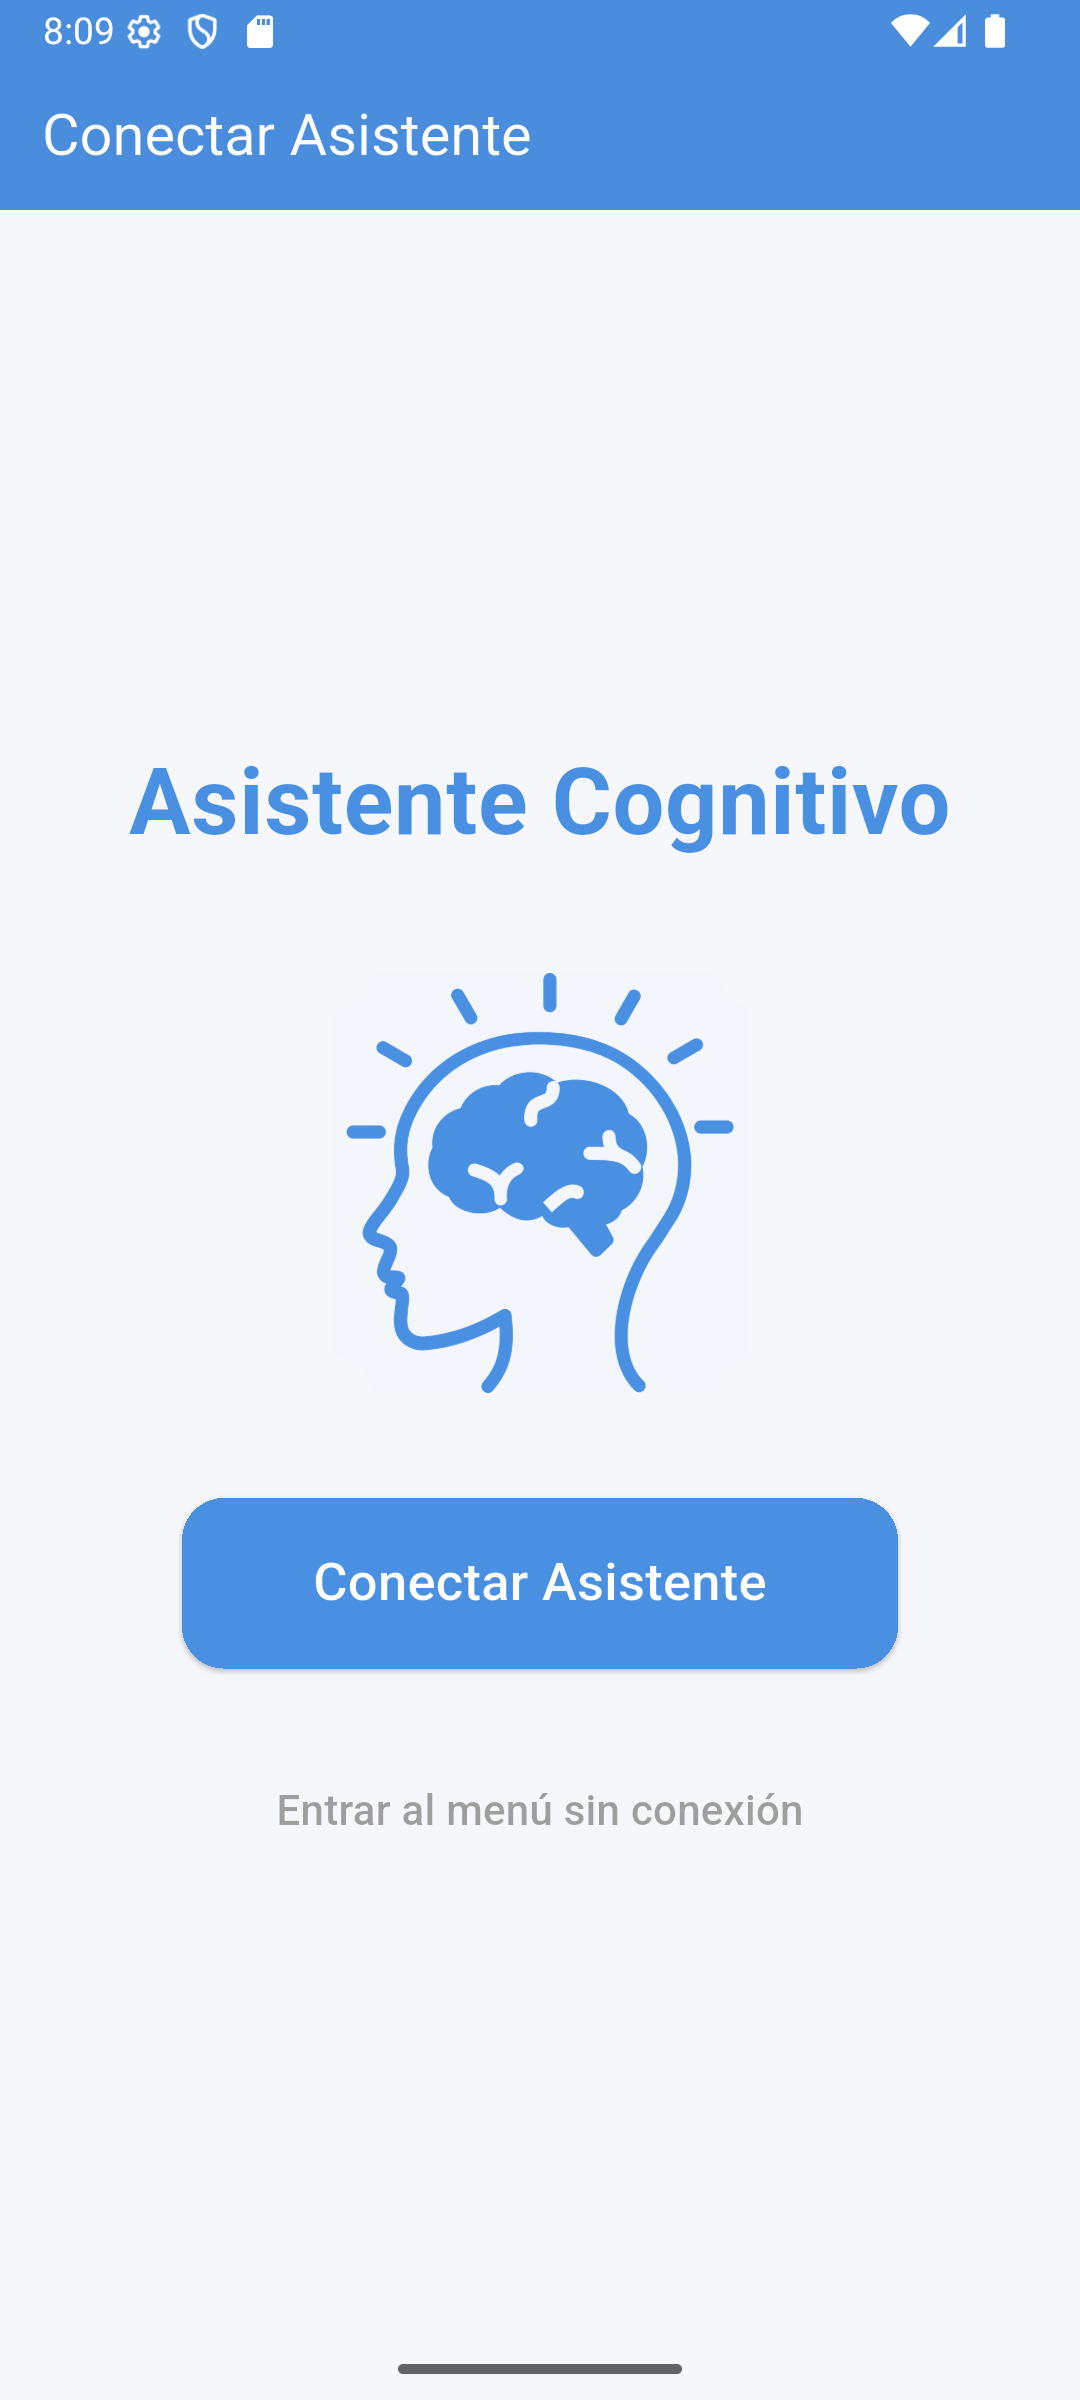
\includegraphics[width=0.5\linewidth]{CHPTRS/CH04_DISEÑO/imagenes/imag_interfaz/inicio.png}
        \caption{Pantalla Conexión}
        \label{fig:interfaz.conexion}
        
    \end{subfigure}
    \hfill
    % Segunda imagen
    \begin{subfigure}{0.5\textwidth}
       

        \centering
        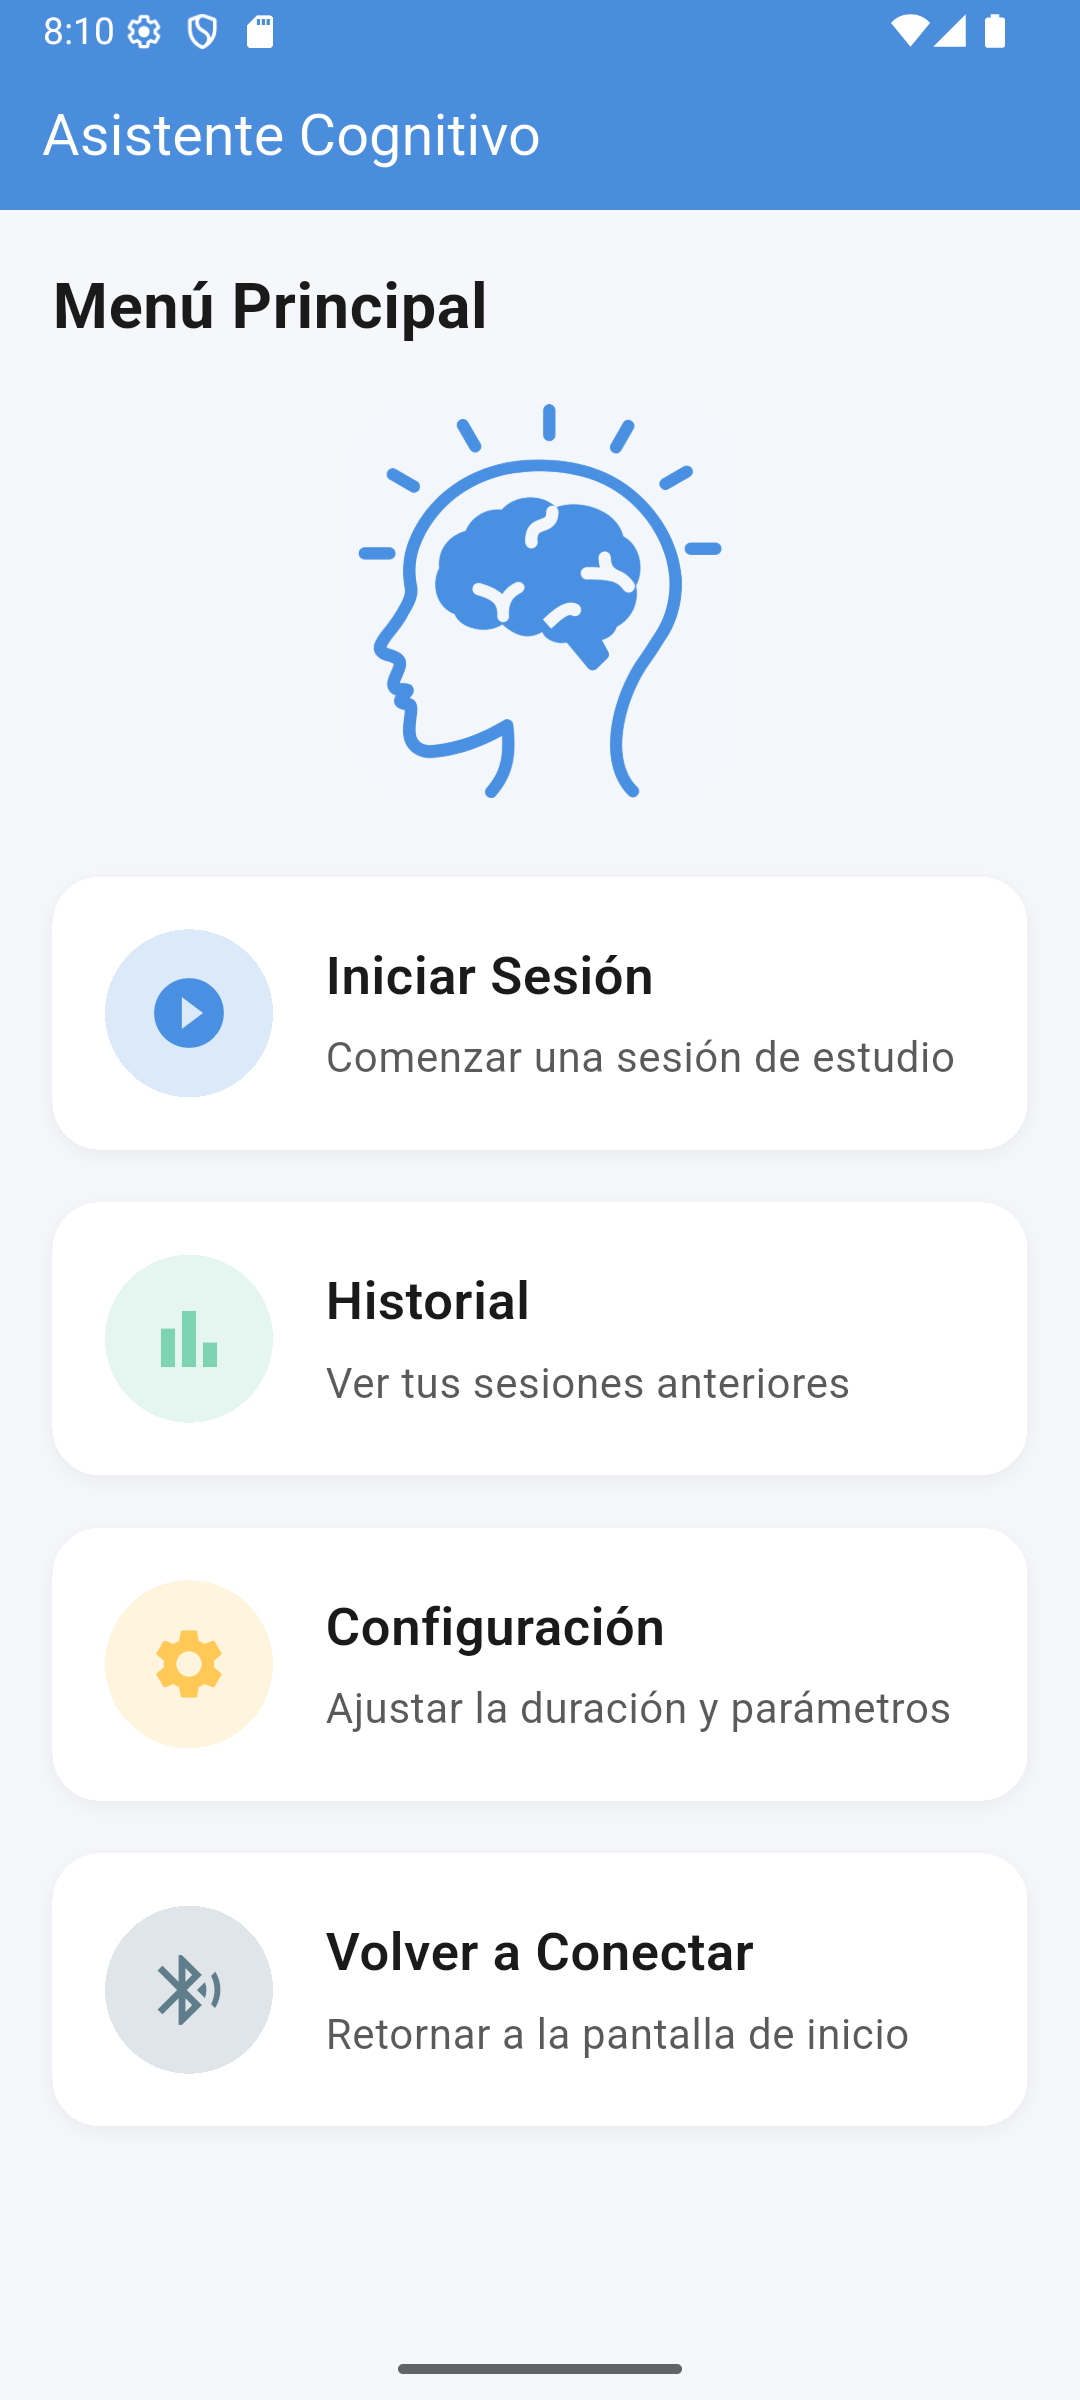
\includegraphics[width=0.4\linewidth]{CHPTRS/CH04_DISEÑO/imagenes/imag_interfaz/MENU PRINCIPAL.png}
        \caption{Menú principal}
        \label{fig:interfaz.menu}
        
    \end{subfigure}
    \caption{Pantallas de Conexión y Menú del Aplicativo}

\end{figure}


\subsubsection{Sesión}
La pestaña Sesión permite ver en tiempo real las métricas que se pueden llegar a obtener del dispositivo durante la sesión de estudio. Estas son la frecuencia cardíaca, el estado de concentración, una gráfica de frecuencia cardíaca con el tiempo y por último un contador que depende de la duración que ha establecido el usuario. En la Figura~\ref{fig:interfaz.sesion} se puede observar la vista de esta pestaña con datos generados aleatoriamente.

\subsubsection{Configuración}
La función de la pestaña de Configuración (ver Figura~\ref{fig:interfaz.conf}) es que el usuario tenga la capacidad de determinar la duración de la sesión de estudio y que este tenga la posibilidad de calibrar el dispositivo de acuerdo a sus datos de frecuencia cardíaca.

\begin{figure}[H]
    \centering
    % Primera imagen
    \begin{subfigure}{0.4\textwidth}
        \centering
        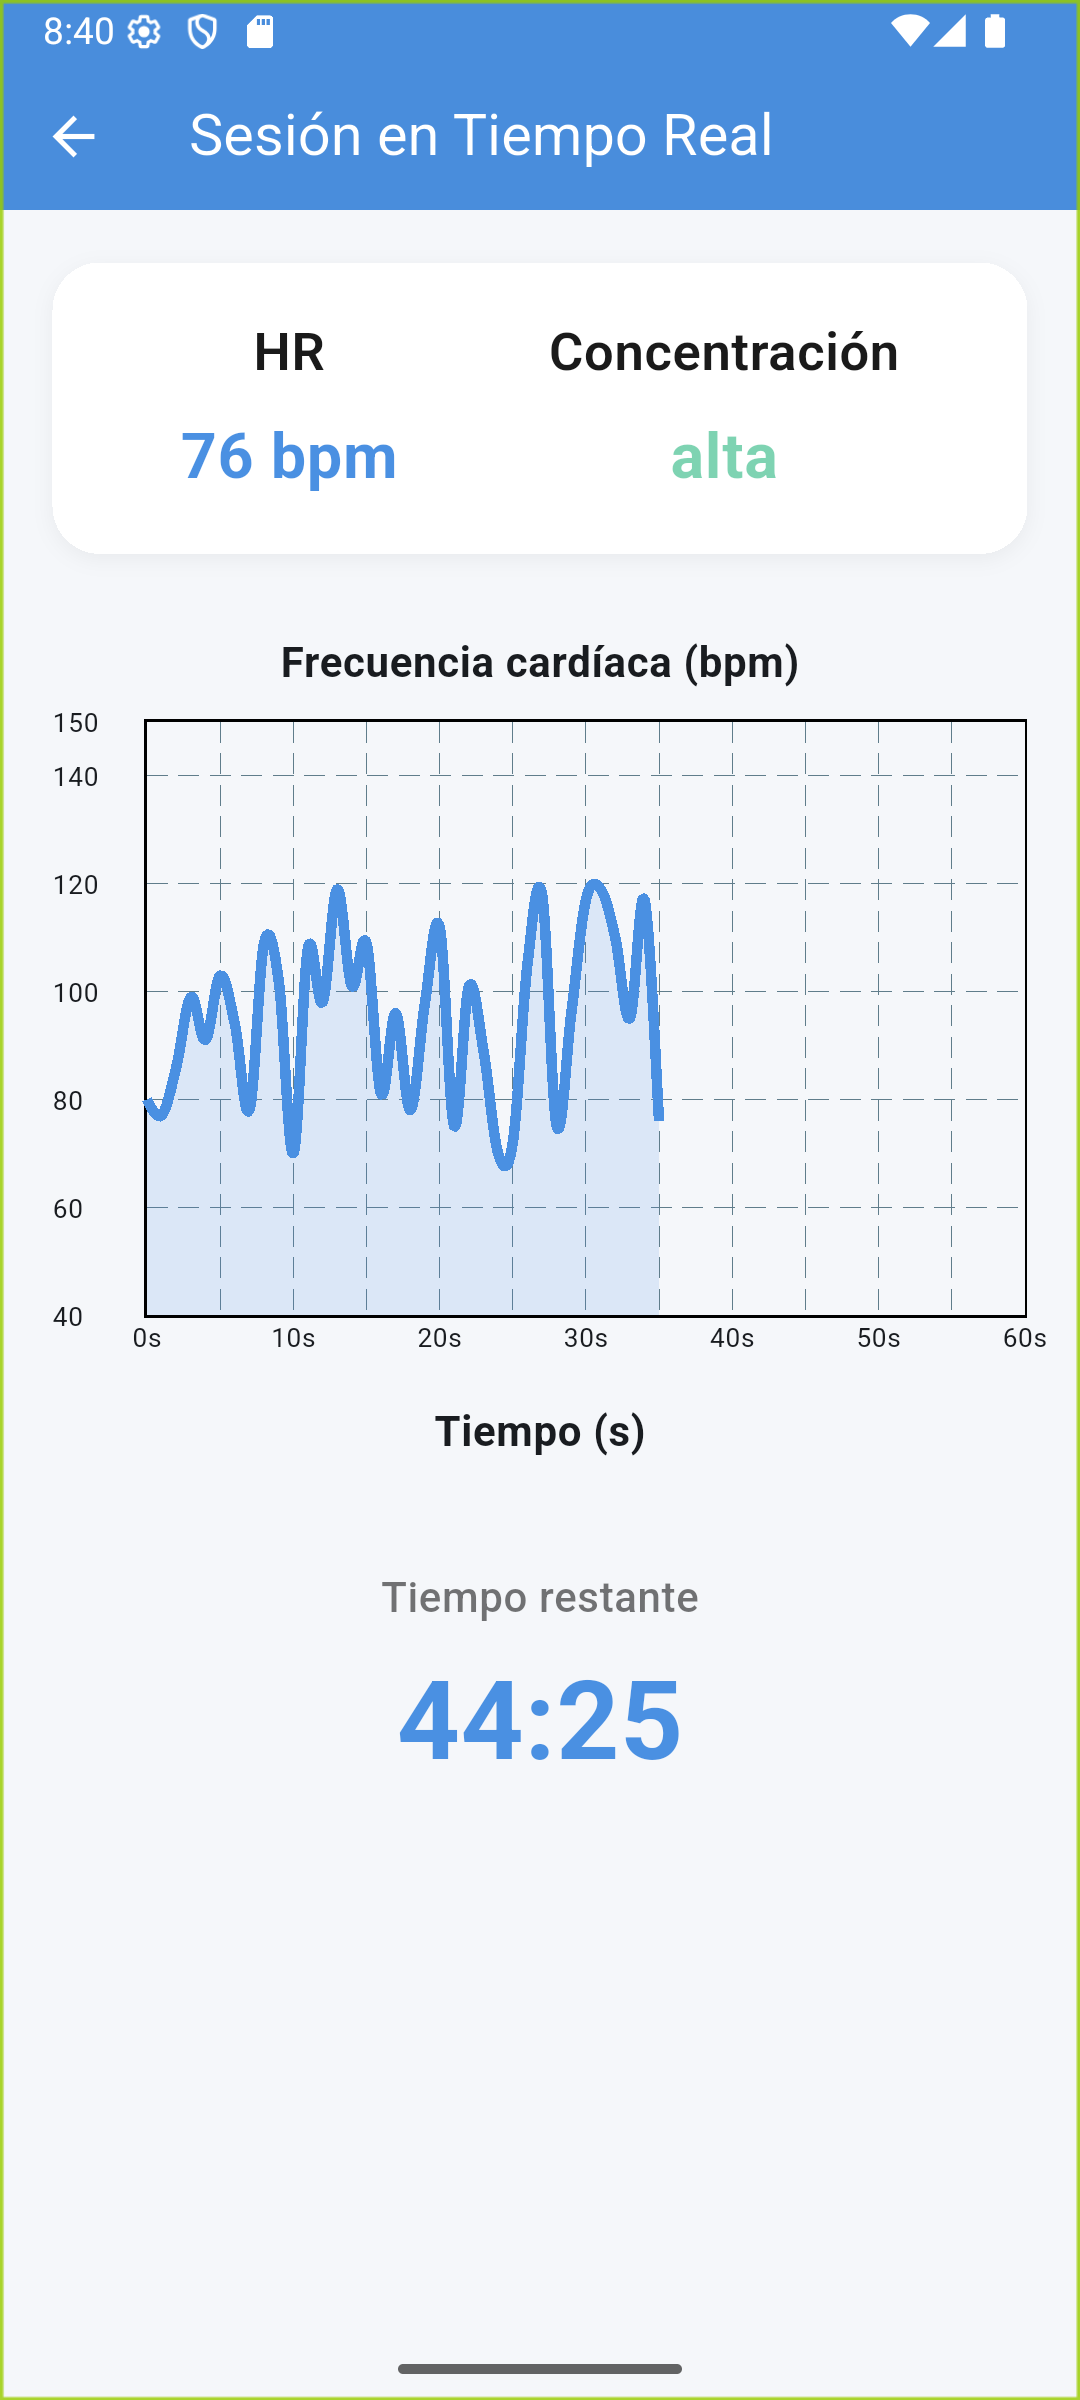
\includegraphics[width=0.5\linewidth]{CHPTRS/CH04_DISEÑO/imagenes/imag_interfaz/Sesion iniciada.png}
        \caption{Pantalla Sesión en progreso}
        \label{fig:interfaz.sesion}
        
    \end{subfigure}
    \hfill
    % Segunda imagen
    \begin{subfigure}{0.5\textwidth}
       

        \centering
        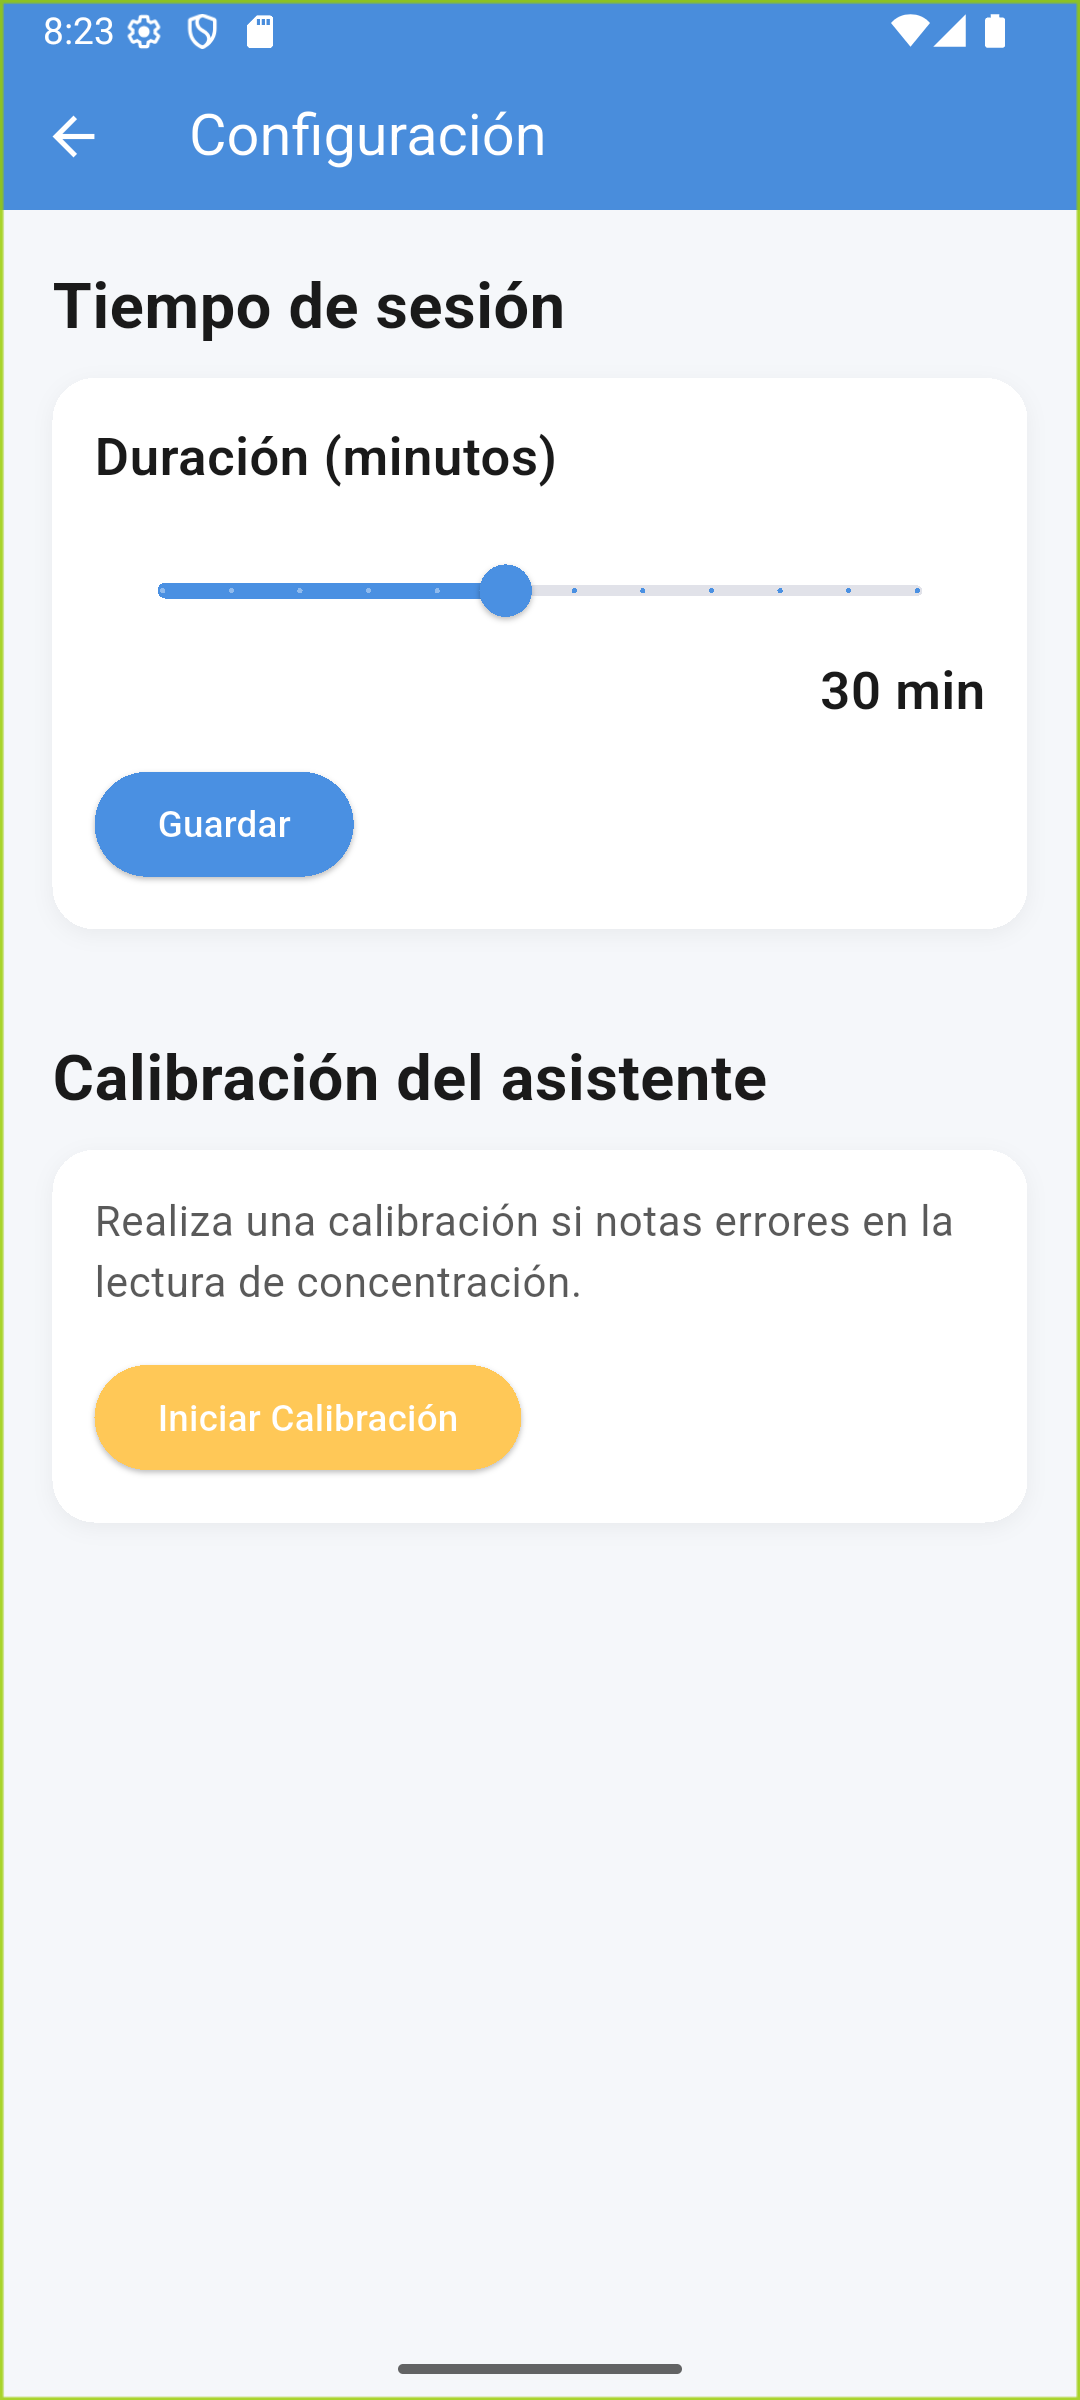
\includegraphics[width=0.4\linewidth]{CHPTRS/CH04_DISEÑO/imagenes/imag_interfaz/configuracion.png}
        \caption{Pantalla de Configuración}
        \label{fig:interfaz.conf}
        
    \end{subfigure}
    \caption{Pantallas de Sesión en proceso y Configuración}

\end{figure}


\subsubsection{Historial}
La pestaña Historial (ver Figura~\ref{fig:interfaz.Historial}) muestra la lista de las sesiones completadas, en ellas se puede observar duración, frecuencia cardíaca promedio, concentración promedio y una barra de progreso que determina cuantas veces el usuario se ha desconcentrado. Asimismo, el usuario es capaz de ingresar a una sesión en particular y observar la gráfica de su frecuencia cardíaca como se puede apreciar en la Figura~\ref{fig:interfaz.sesionEsp}. Además, el aplicativo cuenta con almacenamiento local (en el mismo dispositivo), realizado mediante SQLite que permite almacenar de forma persistente los datos de cada sesión incluso después de cerrar la aplicación.

\begin{figure}[H]
    \centering
    % Primera imagen
    \begin{subfigure}{0.4\textwidth}
        \centering
        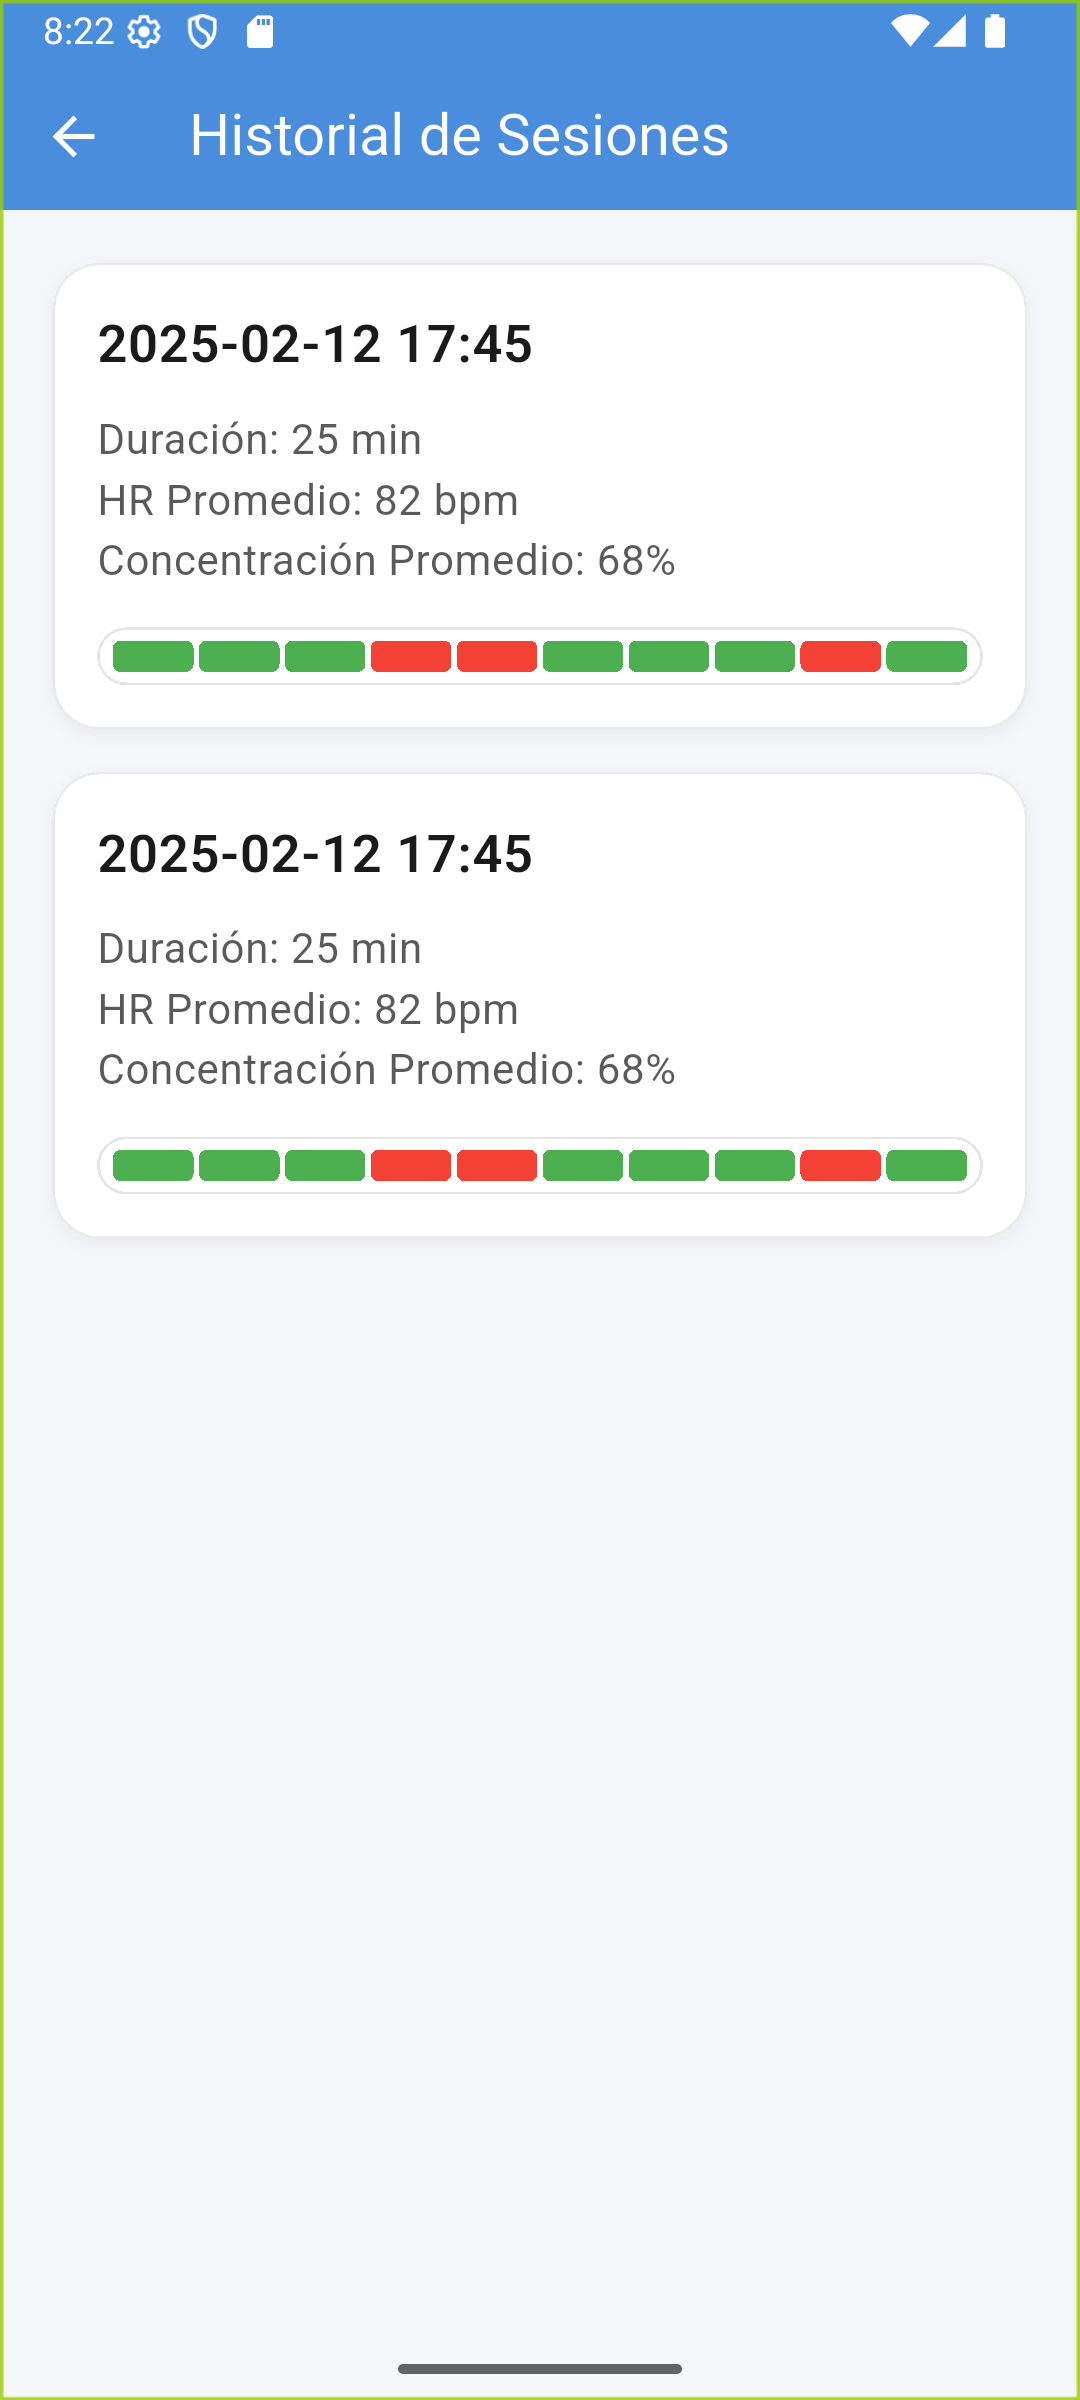
\includegraphics[width=0.5\linewidth]{CHPTRS/CH04_DISEÑO/imagenes/imag_interfaz/Historial.png}
        \caption{Historial general}
        \label{fig:interfaz.Historial}
        
    \end{subfigure}
    \hfill
    % Segunda imagen
    \begin{subfigure}{0.5\textwidth}
       

        \centering
        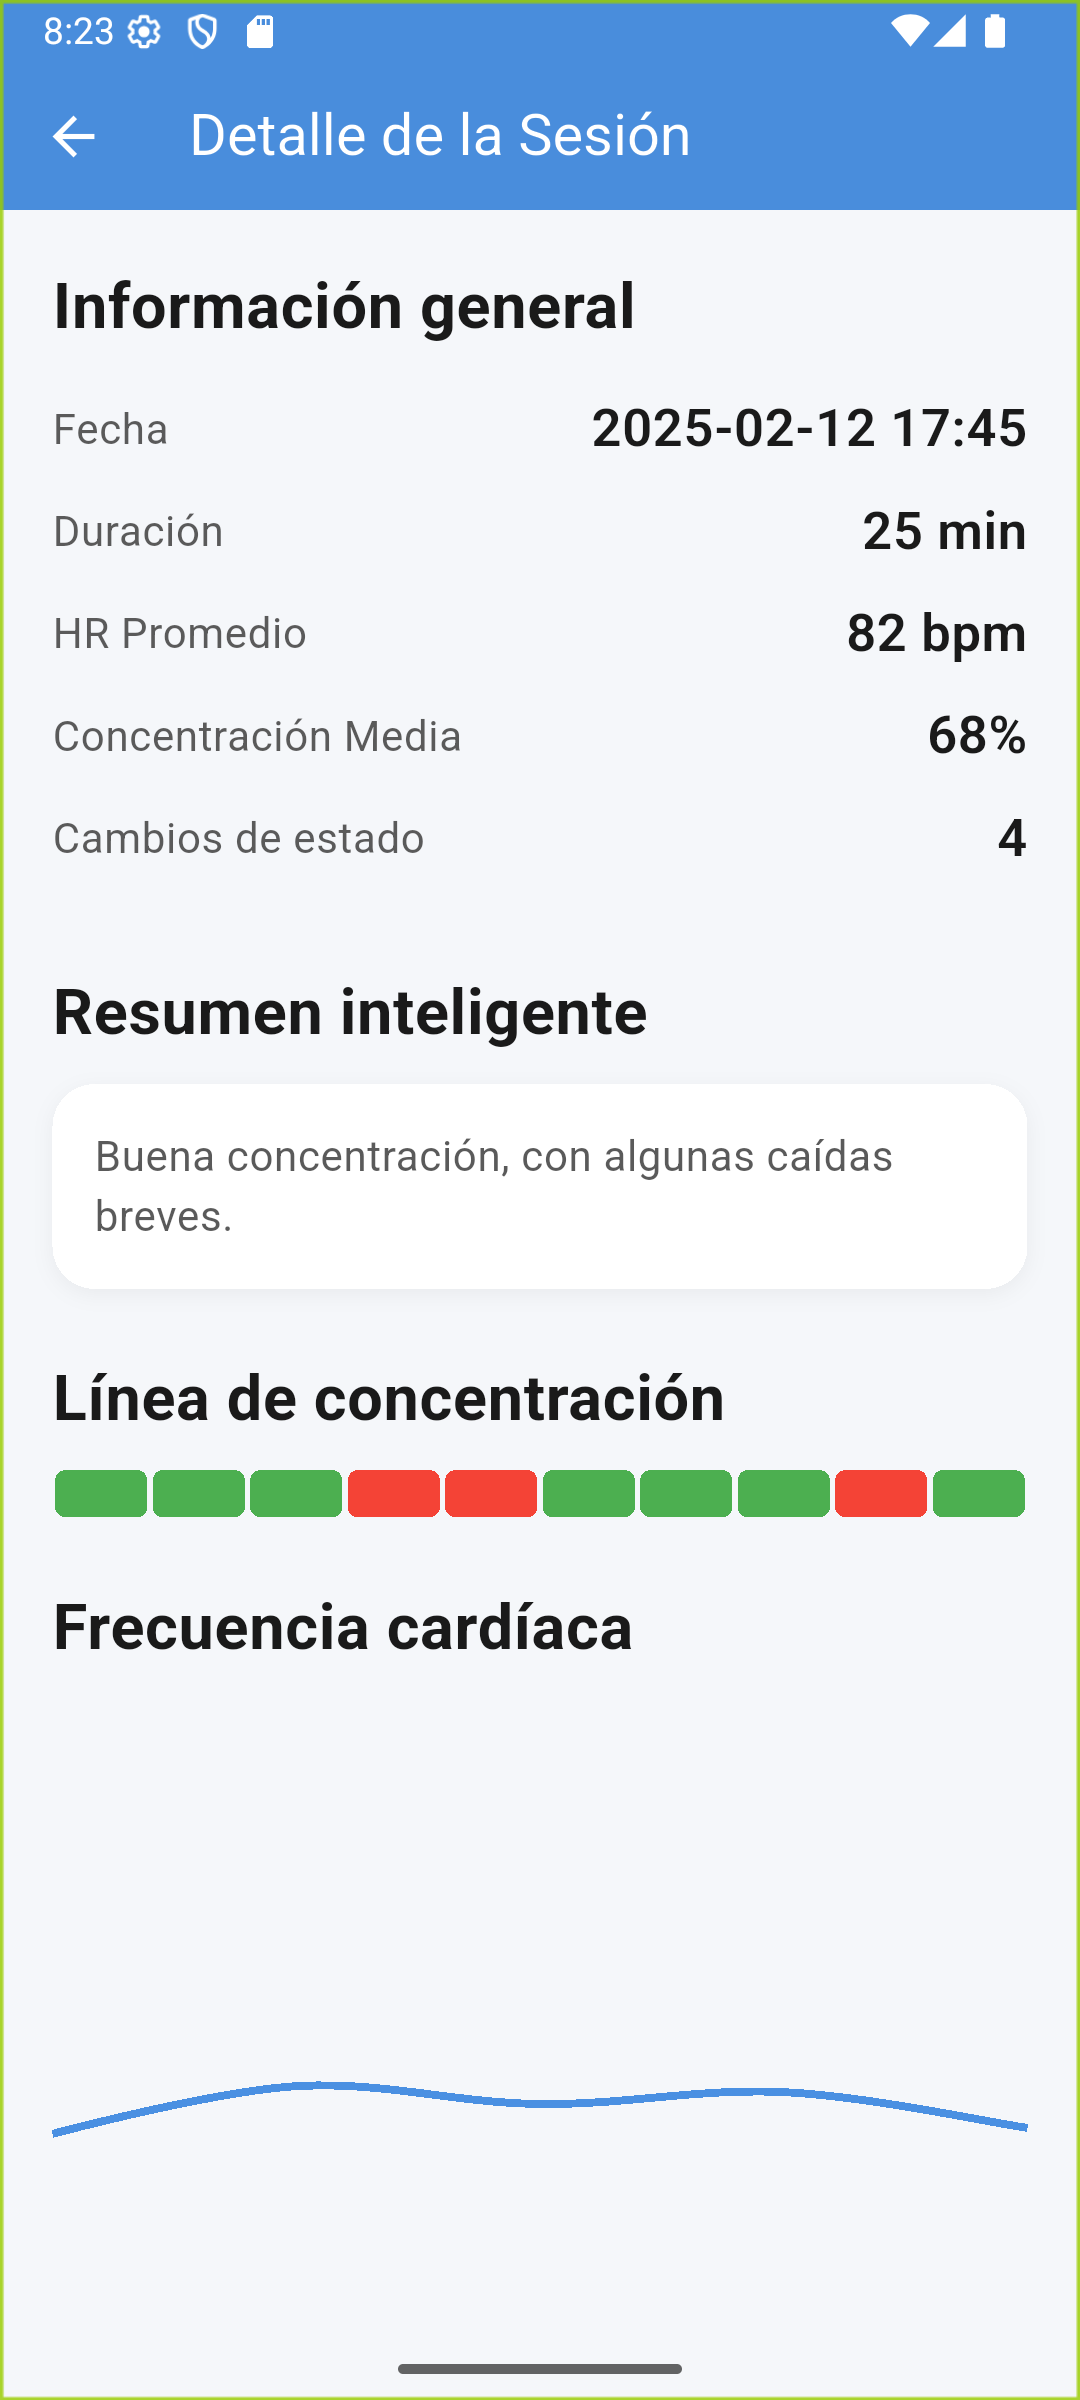
\includegraphics[width=0.4\linewidth]{CHPTRS/CH04_DISEÑO/imagenes/imag_interfaz/Sesion.png}
        \caption{Historial de sesión específica}
        \label{fig:interfaz.sesionEsp}
        
    \end{subfigure}
    \caption{Pantallas de Historial de Sesiones}

\end{figure}
%%%%%%%%%%%%%%%%%%%%%%%
\section{Costos}
En esta sección se presentan los costos para el desarrollo del asistente. Asimismo, se debe recalcar que el diseño del asistente se baso en componentes disponibles localmente y que no se están considerando costos de ensamblaje de los componentes con la carcasa. 
\subsection{Costo de materiales eléctricos}
En la tabla~\ref{tab:4.Costo componentes}, se muestra la estimación de los costos de los componentes electrónicos que se utilizan en el diseño electrónico del dispositivo con un total de S/.109.90. Sin embargo, se tiene que tener en cuenta que no se esta considerando los costos de envió, al cual se le asignará un aproximado de S/.40, obteniendo un costo final de materiales eléctricos de S/.149.90. 

\begin{table}[H]
\centering
\caption{Costo de componentes electrónicos}
\label{tab:4.Costo componentes}
\begin{tabular}{|c|c|c|c|c|} 
\hline
Componente                  & Proveedor         & Precio Unitario (S/.) & Cantidad & Precio Total  \\ 
\hline
Módulo ESP32                & Electromanía      & S/.38               & 1        & S/.38     \\ 
\hline
Sensor MAX30102             & Electromanía      & S/.20                 & 1        & S/.20         \\ 
\hline
Regulador de voltaje MT3608 & Electromanía      & ~S/.5                 & 1        & S/.5          \\ 
\hline
Regulador de voltaje MP1584 & Hi-FI electrónica & S/.3.90               & 1        & S/.3.90       \\ 
\hline
Motor de Vibración          & Hi-FI electrónica & S/.1.70               & 1        & S/.1.70       \\ 
\hline
Modulo de Carga~ HW373      & SAISAC            & S/.4                  & 1        & S/.4          \\ 
\hline
Batería de Litio 1000mAh    & HI-Fi electrónica & S/.11.30              & 1        & S/.11.30      \\ 
\hline
Botón de encendido          & Hi-Fi electrónica & S/.0.80               & 1        & S/.0.80       \\ 
\hline
Transistor 2N3904           & Hi-Fi electrónica & S/.0.20               & 1        & S/.0.20       \\ 
\hline
PCB                         &           PCB Perú        & S/.25                   & 1        & S/.25           \\ 
\hline
\multicolumn{4}{|c|}{Total}                                                        &     S/.109.90          \\
\hline
\end{tabular}
\end{table}
\subsection{Costo de componentes y materiales mecánicos}

En esta sección se detallan las estimaciones de costos de fabricación de la carcasa y la correa. En la Tabla~\ref{tab:4.Costo carcasa} se muestra los costos de fabricación de la carcasa tanto de la parte inferior como de la parte superior. La cotización pertenece a 3Dprint.pe.

\begin{table}[H]
\centering
\caption{Costo de Fabricación de carcasa}
\label{tab:4.Costo carcasa}
\begin{tabular}{|c|c|c|} 
\hline
Componente                  & Cantidad & Precio Total (S/.)  \\ 
\hline
Carcasa-Parte inferior-PETG & 1        & 34         \\ 
\hline
Carcasa-Parte superior-PETG & 1        & 18         \\ 
\hline
\multicolumn{2}{|c|}{Total}            & 52         \\
\hline
\end{tabular}
\end{table}
Asimismo, se deben considerar los elementos de sujeción tanto para la tarjeta como para la carcasa. Esta se encuentra en la Tabla~\ref{tab:4.Costo sujeción}, obteniendo  un total de S/.32.70. Sin embargo, se debe mencionar que la correa de Nylon es vendida por rollo, lo cual daría abasto para múltiples asistentes.

\begin{table}[H]
\centering
\caption{Costo de materiales de sujeción}
\label{tab:4.Costo sujeción}
\begin{tabular}{|c|c|c|c|c|} 
\hline
Componente                                                                           & Proveedor      & Precio Unitario (S/.) & Cantidad & Precio Total(S/.)  \\ 
\hline
\begin{tabular}[c]{@{}c@{}}Inserto roscado para\\impresion 3D con perno\end{tabular} & MTLab          & 0.5                & 4        & 2.0        \\ 
\hline
Correa de Nylon                                                                      & Deming Taguchi & 24                  & 1        & 24         \\ 
\hline
Velcro adhesivo                                                                      & Coto Trapillo  & 3.1                & 2        & 6.20       \\ 
\hline
\multicolumn{4}{|c|}{Total}                                                                                                              & 32.20       \\
\hline
\end{tabular}
\end{table}

Finalmente, se obtiene un costo de materiales mecánicos en total de S/.84.20 considerando ambas tablas previas. Sin embargo, al igual que en los materiales eléctricos, se va a considerar un precio de envió aproximado de S/.40, obteniendo un costo final de S/.124.20. 


\subsection{Costo total}
El costo total se resume en la siguiente Tabla~\ref{tab:4.Costo materiales} con un costo de materiales de S/.234.6, lo cual es un indicatorio que a pesar de enfocarlo a componentes locales, se obtuvo un costo promedio considerando que uno de los requisitos era tener el menor costo posible. 

\begin{table}[H]
\centering
\caption{Costo de materiales Final}
\label{tab:4.Costo materiales}
\begin{tabular}{|c|c|} 
\hline
Materiales            & Precio Total (S/.) \\ 
\hline
Materiales Eléctricos & 109.90     \\ 
\hline
Materiales Mecánicos  & 124.20     \\ 
\hline
Total                 & 234.10      \\
\hline
\end{tabular}
\end{table}


\section{Simulaciones}
\subsection{Carcasa impresa}
Se realizó la impresión de la carcasa con PETG como se puede apreciar en la Figura~\ref{fig:impreso}, se obtuvo el diseño esperado sin inconvenientes. Sin embargo, se tuvo que retirar manualmente las venas producidas como soporte durante la impresión 3D.
\begin{figure}[H]
    \centering
    % Primera imagen
    \begin{subfigure}{0.5\textwidth}
        \centering
        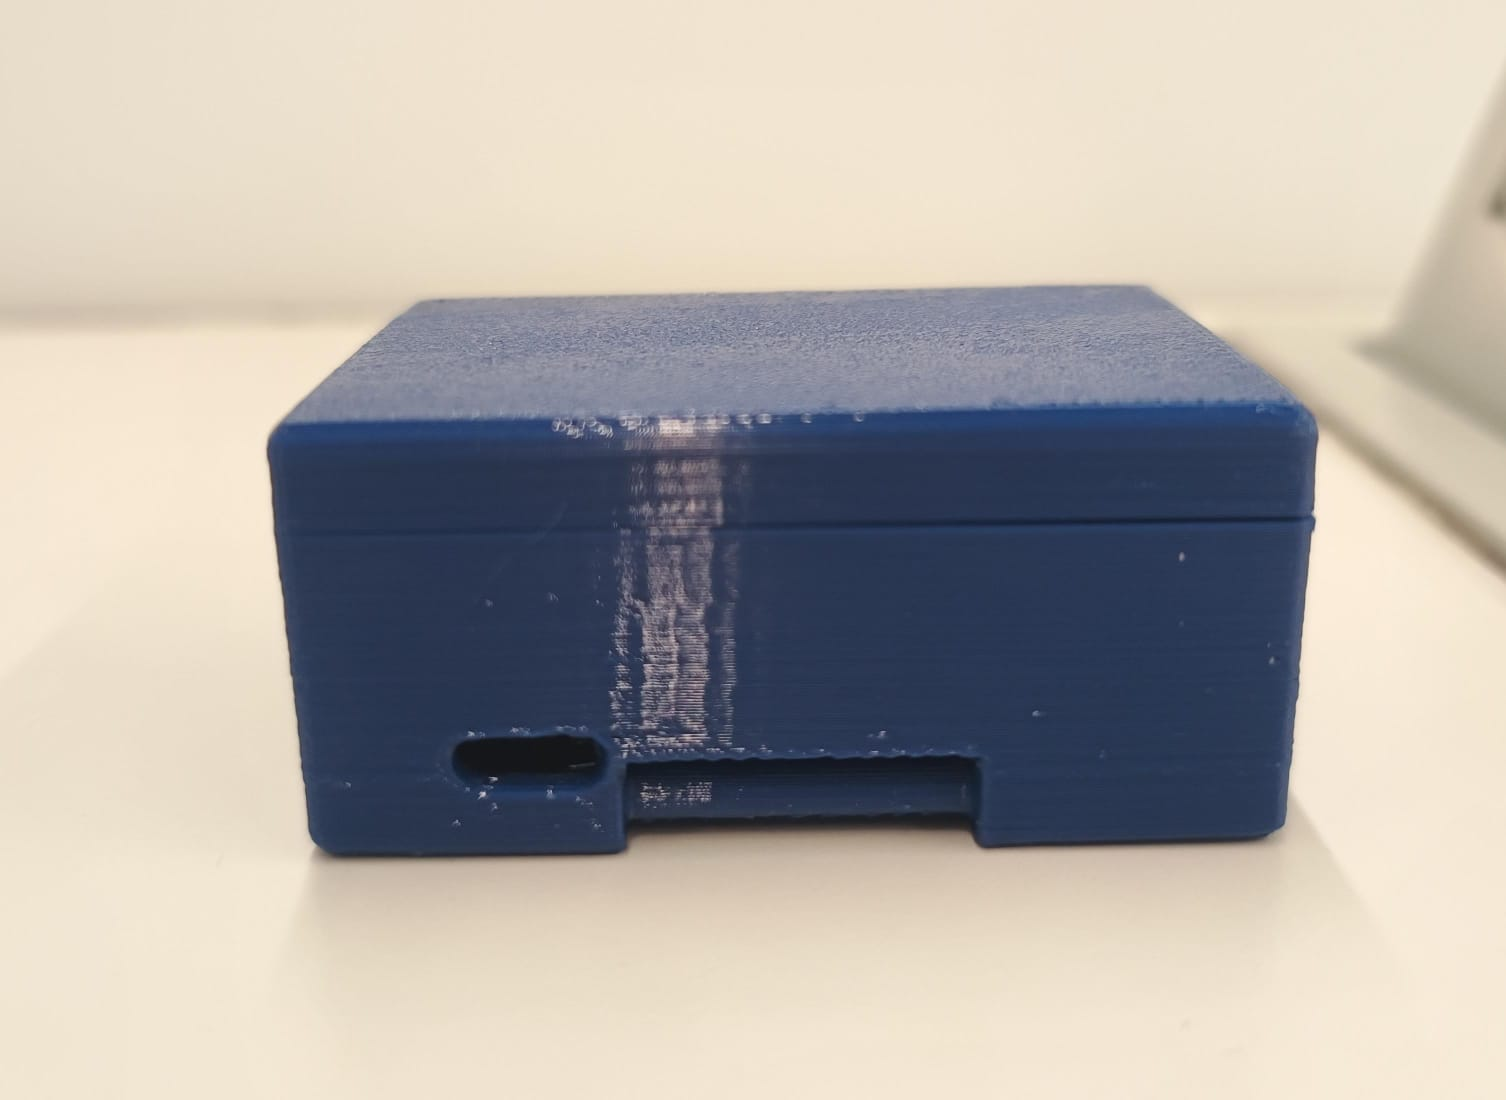
\includegraphics[width=0.75\linewidth]{CHPTRS/CH04_DISEÑO/imagenes/imag_sim/Frontal carcasa.png}
        \caption{Cara frontal}
        \label{fig:interfaz.Historial}
        
    \end{subfigure}
    \hfill
    % Segunda imagen
    \begin{subfigure}{0.4\textwidth}
       

        \centering
        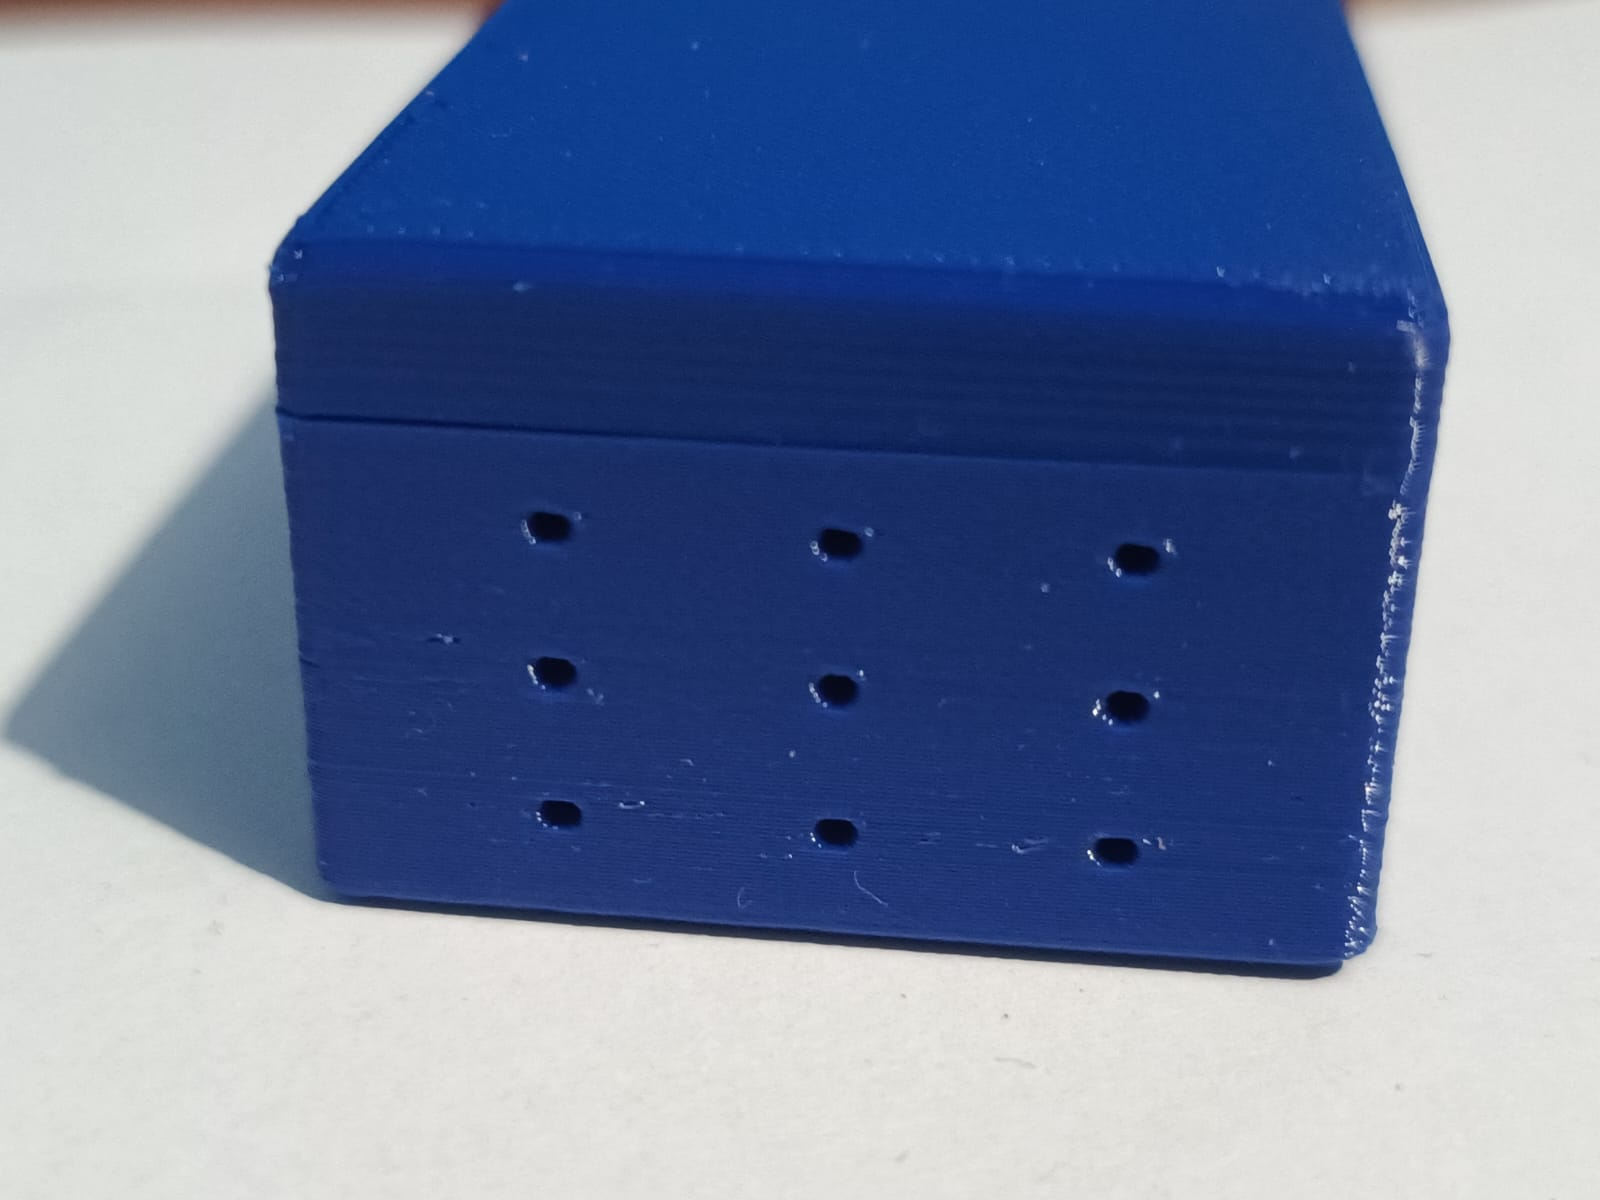
\includegraphics[width=0.85\linewidth]{CHPTRS/CH04_DISEÑO/imagenes/imag_sim/lateral carcasa.png}
        \caption{Cara lateral}
        \label{fig:interfaz.sesionEsp}
        
    \end{subfigure}
    \caption{Carcasa 3D impresa}
    \label{fig:impreso}
\end{figure}
\subsection{Prueba de sujeción de correa}
Para poder simular la sujeción de la correa, se utilizó una báscula manual para maletas que se puede apreciar en la Figura~\ref{fig:sim.bscula}. Esta se colocó en una de las barras circulares como se puede apreciar en la Figura~\ref{fig:sim.basculacolocada}.

\begin{figure}[H]
    \centering
    % Primera imagen
    \begin{subfigure}{0.5\textwidth}
        \centering
        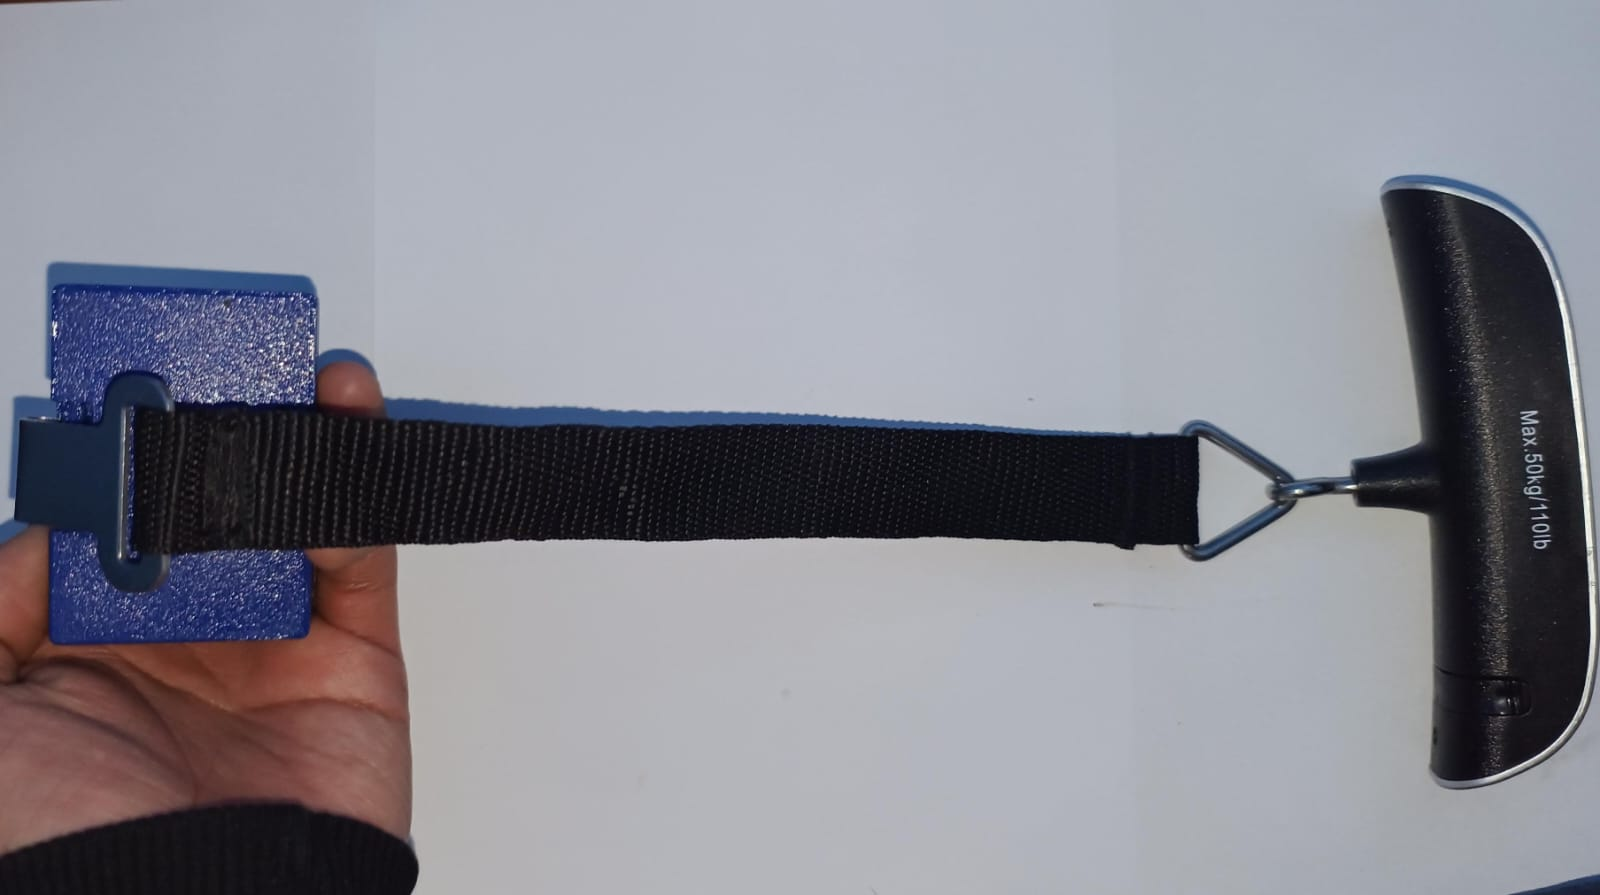
\includegraphics[width=0.75\linewidth]{CHPTRS/CH04_DISEÑO/imagenes/imag_sim/Báscula colocada.png}
        \caption{Báscula colocada}
        \label{fig:sim.basculacolocada}
        
    \end{subfigure}
    \hfill
    % Segunda imagen
    \begin{subfigure}{0.4\textwidth}
       

        \centering
        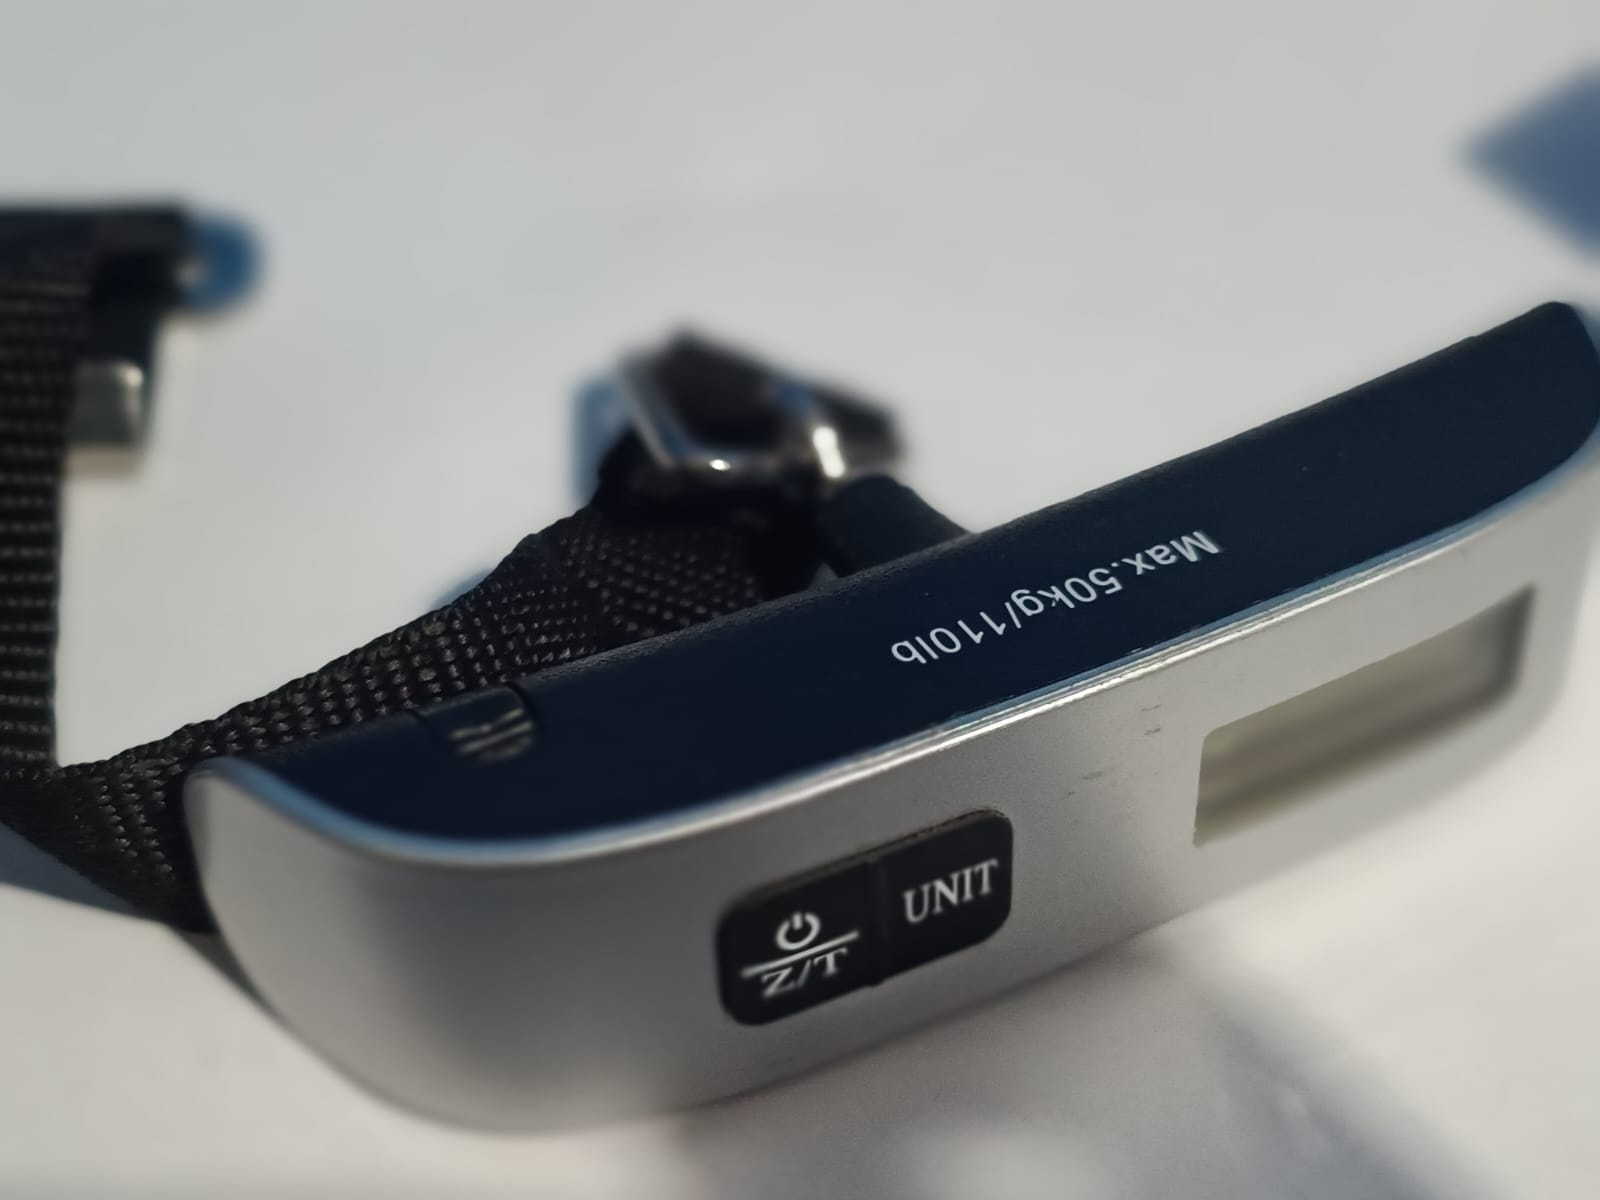
\includegraphics[width=0.85\linewidth]{CHPTRS/CH04_DISEÑO/imagenes/imag_sim/Báscula.png}
        \caption{Báscula digital}
        \label{fig:sim.bscula}
        
    \end{subfigure}
    \caption{Báscula utilizada en pruebas}
    \label{fig:impreso}
\end{figure}

Los resultados son satisfactorios, ya que al momento de realizar la tensión manualmente se obtuvo un valor aproximado de 10 kg como se puede apreciar en la Figura~\ref{fig:sim.sujecion}, lo cual equivale a 98.1N. validando los resultados de los cálculos realizados previamente para las barras circulares con una fuerza de 40N. 
\begin{figure}[H]
    \centering
    % Primera imagen
    \begin{subfigure}{0.5\textwidth}
        \centering
        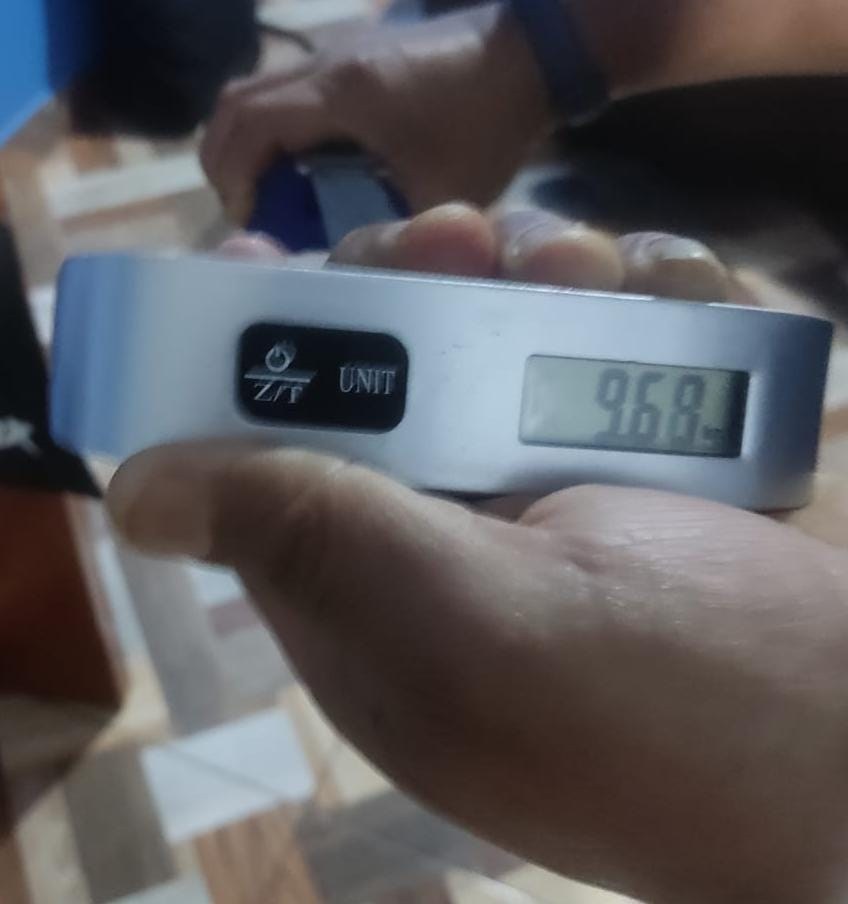
\includegraphics[width=0.75\linewidth]{CHPTRS/CH04_DISEÑO/imagenes/imag_sim/prueba sujecion.png}
        \caption{Tensión en carcasa}
        %\label{fig:sim.basculacolocada}
        
    \end{subfigure}
    \hfill
    % Segunda imagen
    \begin{subfigure}{0.4\textwidth}
       

        \centering
        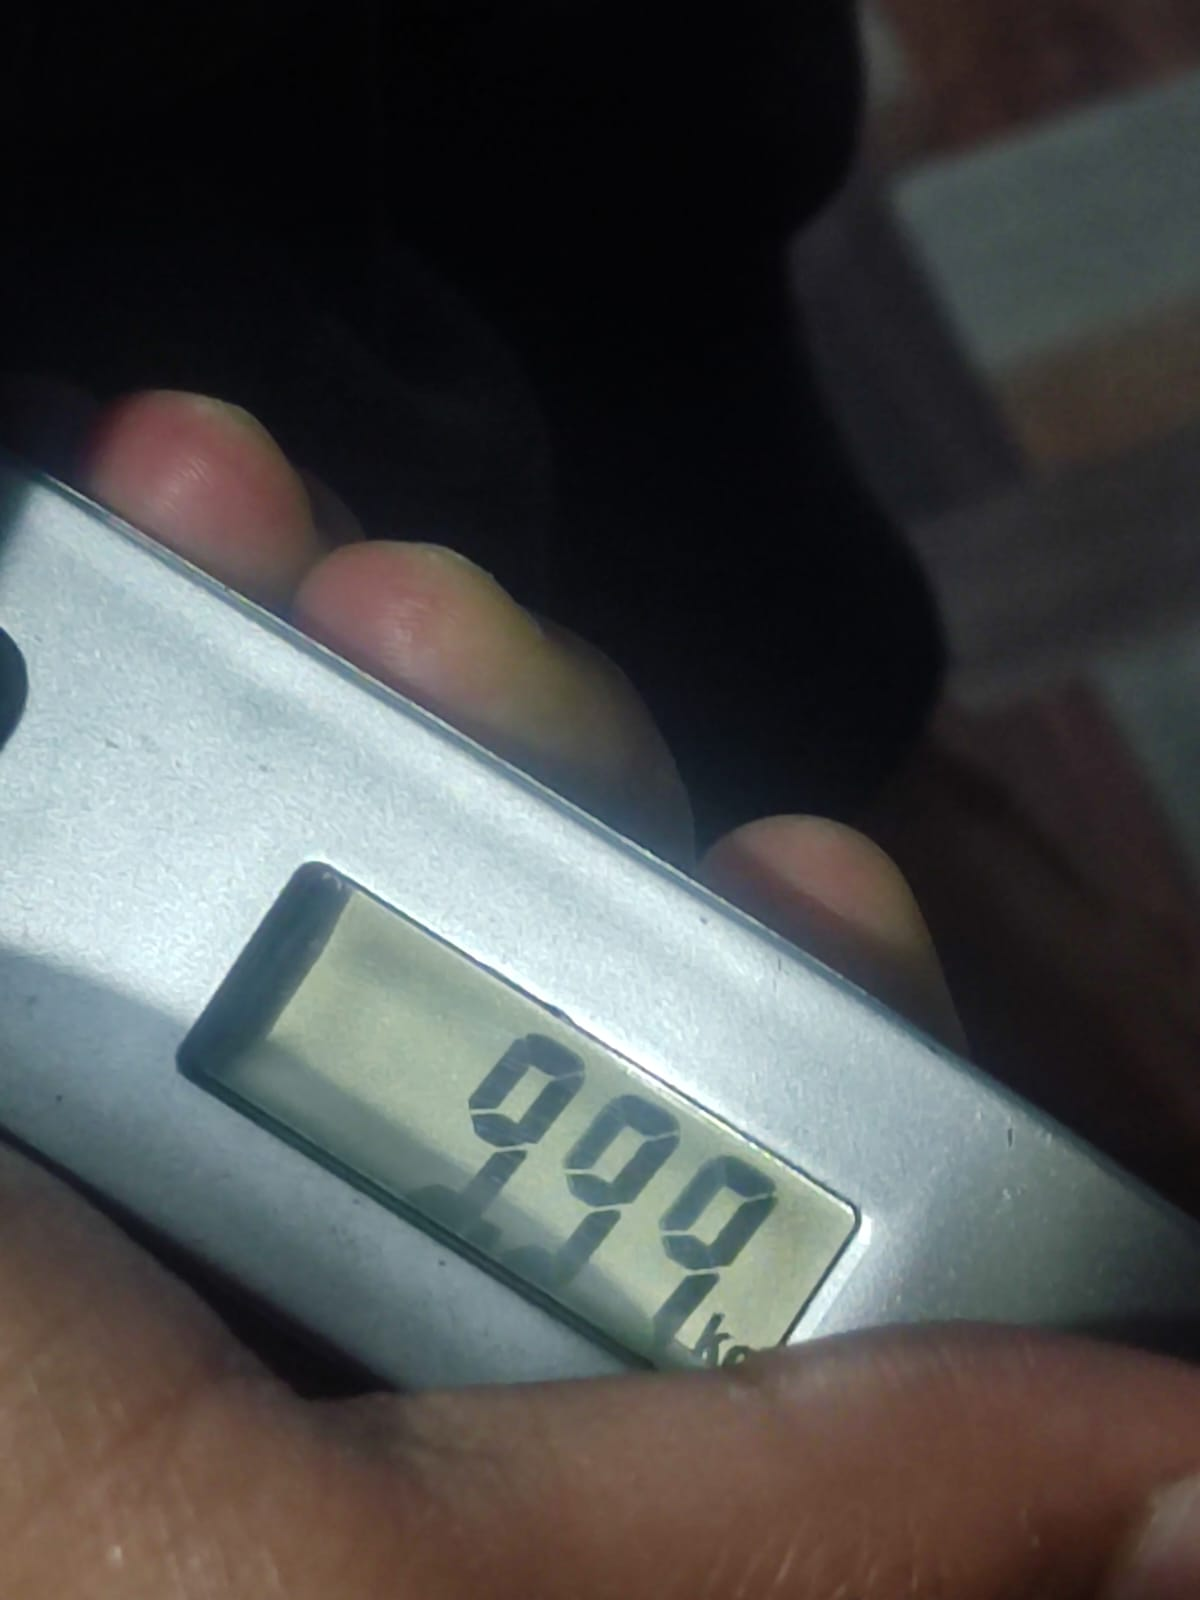
\includegraphics[width=0.8\linewidth]{CHPTRS/CH04_DISEÑO/imagenes/imag_sim/valor sujecion.png}
        \caption{Valor de báscula}
       % \label{fig:sim.bscula}
        
    \end{subfigure}
    \caption{Prueba de sujeción}
    \label{fig:sim.sujecion}
\end{figure}

\subsection{Señal del sensor y estado de concentración}
Para evaluar la señal del sensor MAX30102, este fue colocado en una zona braquial del brazo derecho, como se puede observar en la Figura~\ref{fig:sim.brazo}. Durante las pruebas, la señal fue procesada completamente en el microcontrolador ESP32, realizando la detección de pulsos y estimación del ritmo cardíaco en tiempo real, demostrando que el microcontrolador seleccionado es óptimo para el asistente.\\
\begin{figure}[H]
    \centering
    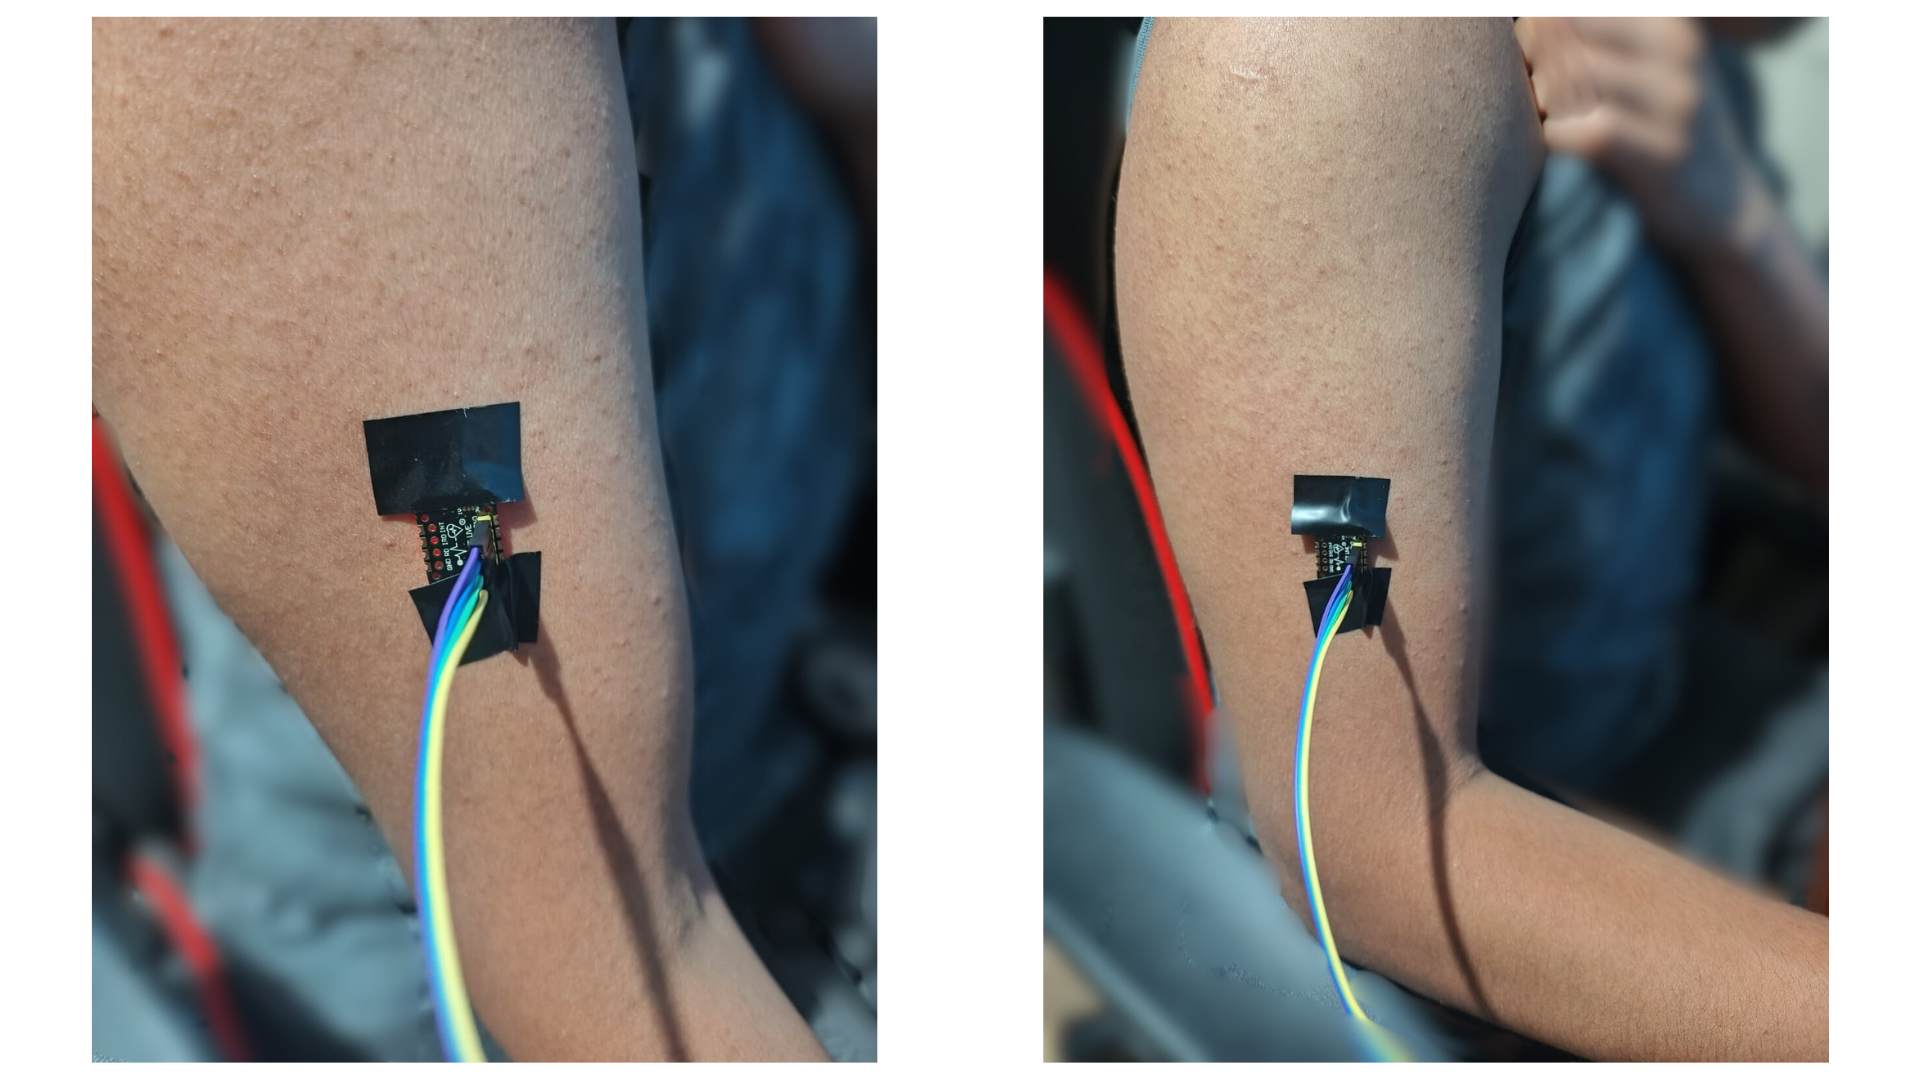
\includegraphics[width=0.8\textwidth]{CHPTRS/CH04_DISEÑO/imagenes/imag_sim/SensorBrazo.png}
    \caption{Sensor MAX30102 colocado en el brazo}
    \label{fig:sim.brazo}
    \captionsetup{justification=centering,margin=1cm}
    \end{figure}
Las pruebas realizadas demuestran  que el largo del cable entre el sensor y el  microprocesador afecta la calidad de la señal, ya que introduce pequeñas variaciones y retrasos en la respuesta, afectando directamente al bus I2C. Sin embargo, el asistente implementa un periodo de calibración basado en la estimación del índice \ac{LF}/\ac{HF}, el cual compensa adecuadamente estas variaciones iniciales (ver Figura~\ref{fig:sim.resultados}). Por ello, el asistente puede adaptarse al patrón fisiológico de cada usuario.

    
\begin{figure}[H]
    \centering
    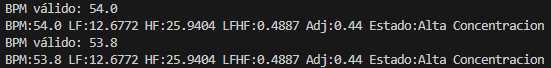
\includegraphics[width=0.8\textwidth]{CHPTRS/CH04_DISEÑO/imagenes/imag_sim/resultados.png}
    \caption{Resultados de clasificación}
    \label{fig:sim.resultados}
    \captionsetup{justification=centering,margin=1cm}
\end{figure}
